\documentclass[a4paper,12pt,twoside]{article}
\tolerance=1000 \hbadness=10000 \raggedbottom
\usepackage{graphicx}
\usepackage{lscape}
\usepackage{rotating}
\usepackage{longtable}
\usepackage{tabularx}
\usepackage{amsmath,latexsym,amssymb}
\usepackage{setspace}
\usepackage{euscript}
\usepackage{lscape,fancyhdr}
\usepackage{float,times}
\usepackage{multirow}
\usepackage{xcolor}
\usepackage{multicol}
\usepackage{color}
\usepackage[export]{adjustbox}
\usepackage{hhline}
\usepackage{rotating}
\usepackage{placeins}
\usepackage{longtable}
\usepackage{setspace}
\usepackage{ragged2e}
\usepackage{subcaption}
\usepackage{euscript}
\usepackage{lscape,fancyhdr}
\usepackage{float,times}
\usepackage{amstext}
\usepackage{amsmath}
\usepackage{multirow,array}
\usepackage[backend=bibtex]{biblatex}
\bibliography{ref.bib}
\newcolumntype{a}{>{\columncolor{Gray}}c}
\def\MARU#1{\leavevmode\setbox0\hbox{$\bigcirc$}%
\copy0\kern-\wd0\hbox to\wd0{\hfil{\scriptsize#1}\hfil}}
\usepackage[top=2.5cm, left=3cm, right=3cm]{geometry}%Used for marigins
%\usepackage{ccaption}
%\makeatletter
%\makeatother\captionnamefont{\fontseries{bc}}
%\renewcommand{\figurename}{\bf{Figure~}}
%\renewcommand{\tablename}{\bf{Table-}}
%\setlength{\unitlength}{0.4in} \setlength{\textheight}{24.5cm}
%\setlength{\textwidth}{16cm}
%\newcommand{\newsection}[1]{\setcounter{equation}{0} \setcounter{secn}{0}\section{#1}}
%\renewcommand{\labelenumi}{\theenumi)}
%\addtocounter{secnumdepth}{3}
%\newcommand\T{\rule{0pt}{2.6ex}}
%\newcommand\B{\rule[-1.2ex]{0pt}{0pt}}
%------------------------------------------------
%------------------------------------------------
%------------------------------------------------
%------------------------------------------------
%------------------------------------------------
%------------------------------------------------
%------------------------------------------------
\begin{document}
\pagestyle{empty} 
\begin{center}
{\Large \bf  Deep Learning based COSMIC-2 Radio Occultation Atmospheric Profile Retrieval}
\end{center}
\vspace{0.5cm}
\begin{center}
\resizebox{9cm}{8cm}{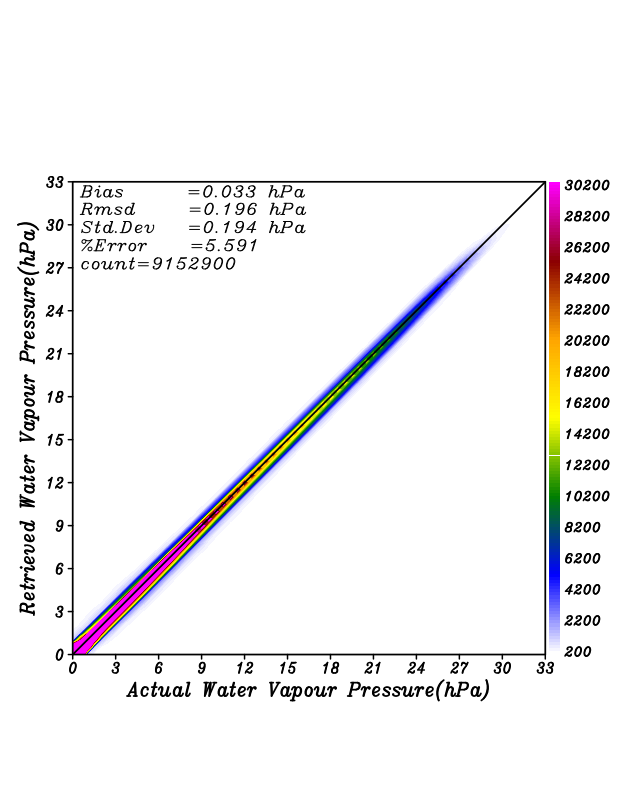
\includegraphics{/Users/soumilhooda/Desktop/COSMIC_REPORT/NEW-FIGURES/cover.png}}\\
\end{center}
\begin{center}
Report submitted for completion of training \\
Satellite Meteorlogy and OceAnography Research and Training - \textbf{SMART} \\
Programme of Space Applications Centre
\end{center}
\vspace{0.5cm}
\begin{multicols}{2}
\begin{center}
	Submitted by \\
	\begin{large}
		\textbf{Soumil Hooda} \\
	\end{large}
	B.E. EEE and M.Sc. Physics \\
	BITS Pilani\\
	 Hyderabad \\
\end{center} 

\begin{center}
	Under the guidance of \\
	\begin{large}
		\textbf{Dr. Satya Prakash Ojha} \\
	\end{large}
	SCI/ENG-SF \\
	PSD/BPSG/EPSA\\
	Space Applications Centre (ISRO) \\
\end{center}

\end{multicols}
%\begin{center}
%Submitted by \\
%\begin{large}
%\textbf{Soumil Hooda} \\
%\end{large}
%(Registration Number RS00415) \\
%B.E. Electrical and Electronics and M.Sc. Physics \\
%BITS Pilani, Hyderabad
%\end{center}
%\vspace{0.05cm}
%\begin{center}
%Under the guidance of \\
%\begin{large}
%\textbf{Dr. Satya Prakash Ojha} \\
%\end{large}
%SCI/ENG-SF \\
%PSD/BPSG/EPSA\\
%Space Applications Centre (ISRO), Ahmedabad \\
%\end{center}
%\vspace{1.5cm}
%\begin{center}
%Institution\\
%\begin{large}
%\textbf{BITS Pilani}\\
%\end{large}
%Hyderabad - 500078\\
%Telangana 
%\end{center}
%\vspace{1.5cm}
\begin{center}
\resizebox{6cm}{4cm}{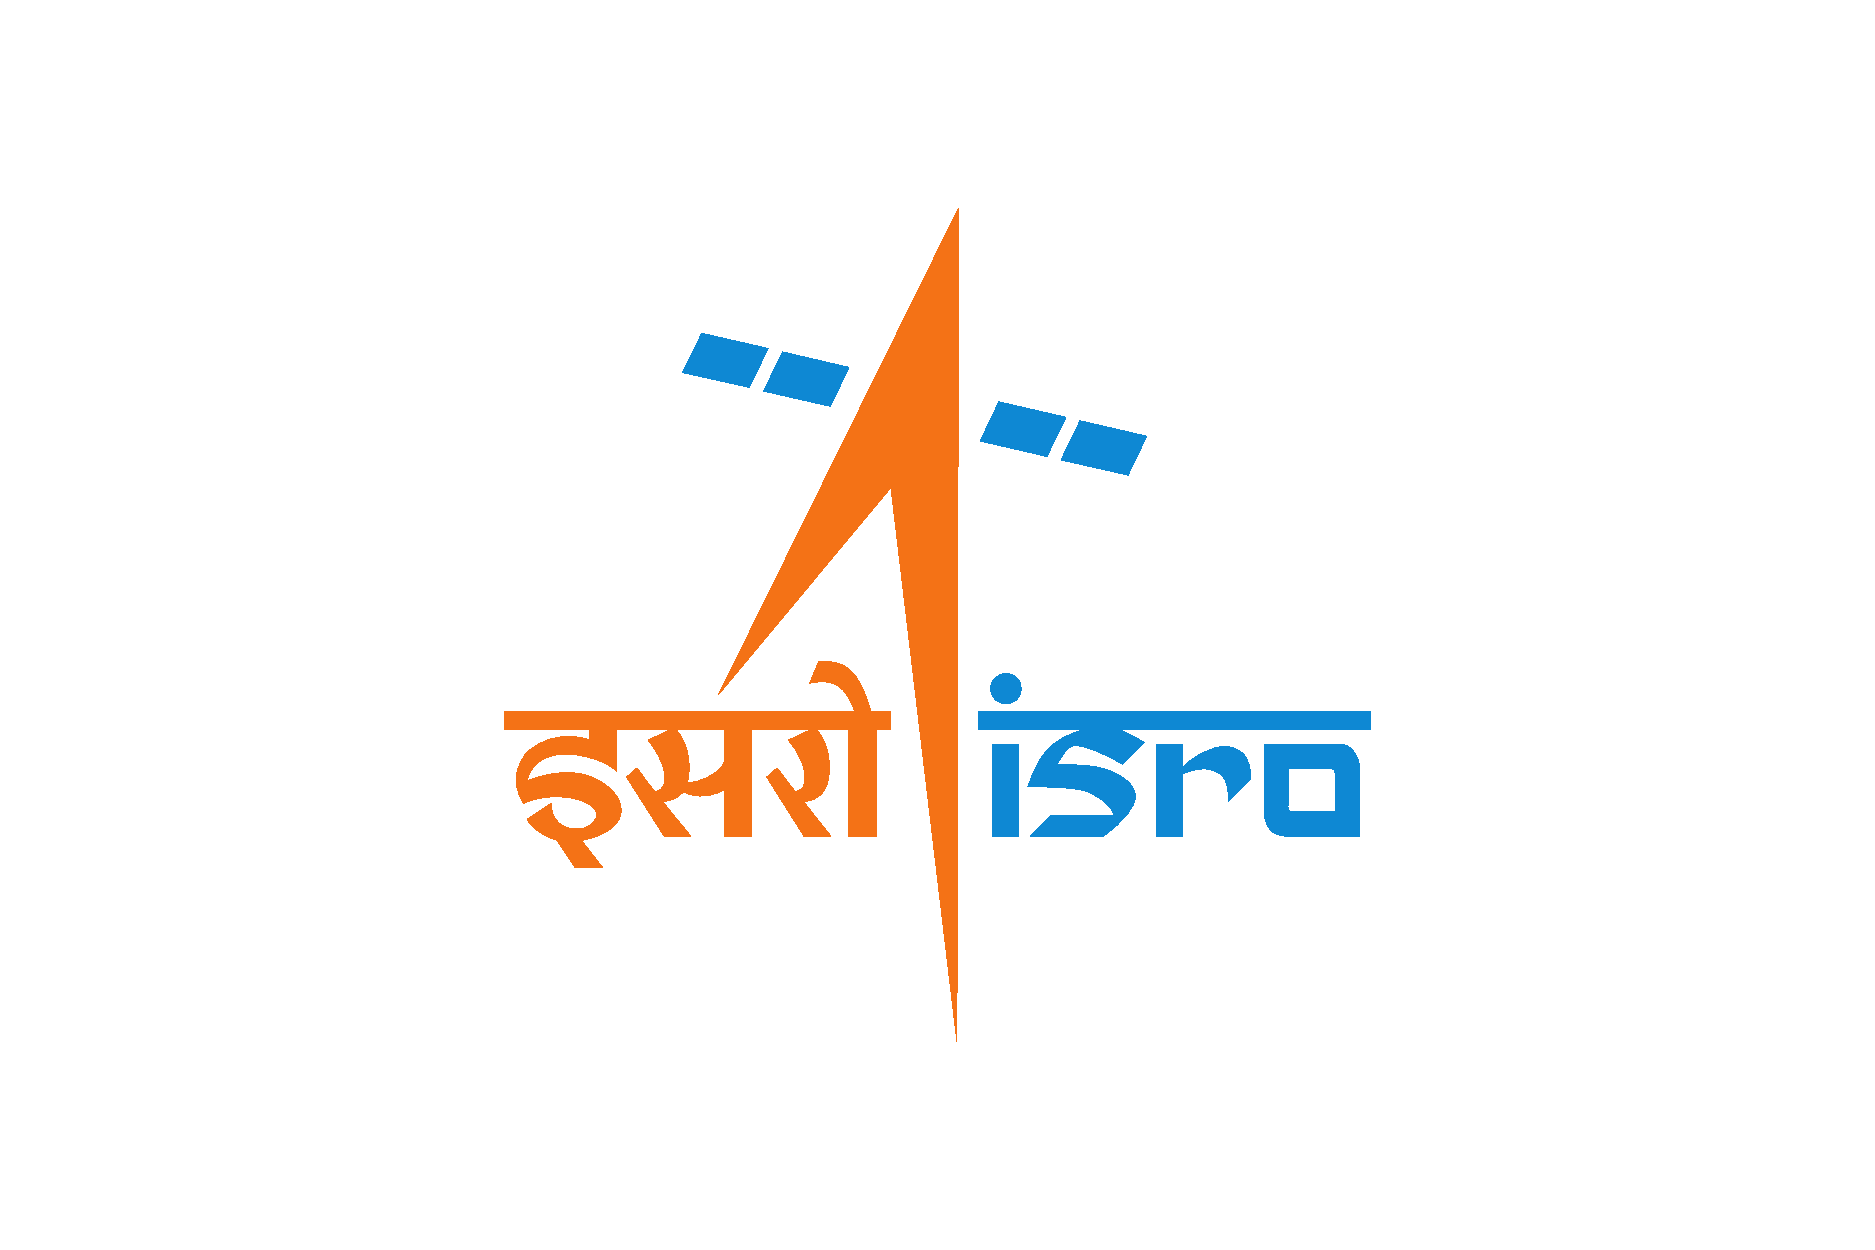
\includegraphics{/Users/soumilhooda/Desktop/COSMIC_REPORT/isro.pdf}}\\
\begin{large}
\textbf{Space Applications Centre\\
Indian Space Research Organisation\\
Ahmedabad-380015, India}\\
\end{large}
June 2022 - August 2022
\end{center}

\newpage
\begin{center}
\begin{LARGE}
Acknowledgement \\	
\end{LARGE}
\begin{center}
\justifying 
\noindent I am extremely grateful to Space Applications Centre (ISRO), Ahmedabad for providing me with the opportunity to work on an amzing problem. I would like to thank Dr. S P Vyas (Head, Scientific Research and Training Division (SRTD)-RTCG/MISA) and the organisers of the Satellite Meteorlogy and OceAnography Research and Training  programme. I would like to provide gratitude to Dr. Satya Prakash Ojha (PSD/BPSG/EPSA/SAC/ISRO) and Dr. Randhir Singh (ASD/AOSG/EPSA/SAC/ISRO) for the enriching learning experience working on a problem together. I am also indebt of the Research, Outreach and Training Coordination Group, Management and Information Systems Area  and all staff members of Space Applications Center (ISRO), Ahmedabad for the continued support throughout. I would also like to thank Mr. Jai Gopal Singla (SIPG/SAC/ISRO) for providing with his computational resources. I would also like to thank Dr. Sarmistha Banik (HoD, Physics Department, BITS Pilani, Hyderabad), for enabling this opportunity for me. \\
\end{center}
\end{center}


\newpage
\begin{center}
\begin{large}
	\textbf{Scientific Research and Training Division (SRTD)} \\
\end{large}
\begin{large}
	\textbf{Research, Outreach and Training Coordination Group (RTCG)} \\
\end{large}
\begin{large}
	\textbf{Management and Information Systems Area (MISA)} \\
\end{large}
\end{center}
\vspace{0.5cm}
\begin{center}
\begin{Large}
\underline{\textbf{CERTIFICATE}} \\
\end{Large}
\end{center}
\vspace{1.5cm}
\begin{center}
	\justifying
This is to certify that \textbf{Mr. Soumil Hooda}, a student of B.E. (Electrical and Electronics) and M.Sc. (Physics) of BITS Pilani, Hyderabad, Telangana has completed a three month (1st June 2022 - 31st August 2022) project on "\textbf{Deep Learning based COSMIC-2 Radio Occultation Atmospheric Profile Retrieval}" under the supervision of Dr. Satya Prakash Ojha, Scientist-SF, PSD/BPSG/EPSA, Space Applications Centre (ISRO), Ahmedabad. The research work was carried out through the Scientific Research and Training Division (SRTD) of Space Applications Centre, Ahmedabad. 
\end{center}


\pagenumbering{arabic} 
\newpage
\begin{center}
\begin{LARGE}
Abstract\\
\end{LARGE}
 \begin{center}
 	\justifying
	Accurate and reliable data on tropospheric temperature and water vapour profiles are crucial for studies of weather and climate. Among the sensors used to assist tropospheric observations, the Global Navigation Satellite System (GNSS) Radio Occultation (RO) technology stands out because it provides precise and excellent meteorological profiles. RO, a form of active limb sounding used by the GNSS, involves GNSS satellites transmitting signals that are then picked up by a GNSS receiver on a low-earth orbiter (LEO) satellite as they pass through the Earth's atmosphere. The atmospheric refractivity profile is accurately produced by GNSS RO. Common techniques (like variational) to drive atmospheric profiles of temperature, water vapour pressure, and pressure require knowledge of the atmospheric condition beforehand (e.g. water vapour pressure, temperature and pressure). By training two Artificial Neural Network (ANN) models using simulated data, we hope to eradicate this dependency in this study. The wetPf2 dataset derived from COSMIC-2 (Formosa Satellite-7/Constellation Observing System for Meteorology, Ionosphere and Climate-2 mission) is used to extract the atmospheric temperature, pressure, and water vapour profiles. A more precise and recently published three-term refractivity formulation is employed to model the corresponding refractivity using the thermodynamic profiles from wetPf2. The inputs to our ANN model are the simulated refractivity, latitude, longitude, height, and month, and the target is the thermodynamic profiles. The model is trained and tested using data from the year 2020, and the results are encouraging. Temperature, pressure, and water vapour pressure have roots mean square errors (RMSE) that are, respectively, 1.28 K, 1.26 hPa, and 0.19 hPa when averaged vertically. Additionally, a completely independent data set obtained in 2021 is used to evaluate the model, and while the retrieval errors are slightly larger, they are still within accepted limits. The vertically averaged root mean square error (RMSE) for the independent data is 1.82 hPa for pressure, 1.64 K for temperature, and 0.24 hPa for water vapour pressure. The retrieval errors for temperature and pressure in this study are comparable to those  achieved by the earlier studies, while the retrieval errors for water vapour are substantially lower in this study. \\
\end{center}
\end{center}
%\newpage
%\vspace*{3cm}
%\begin{figure}[H]
%\centering
%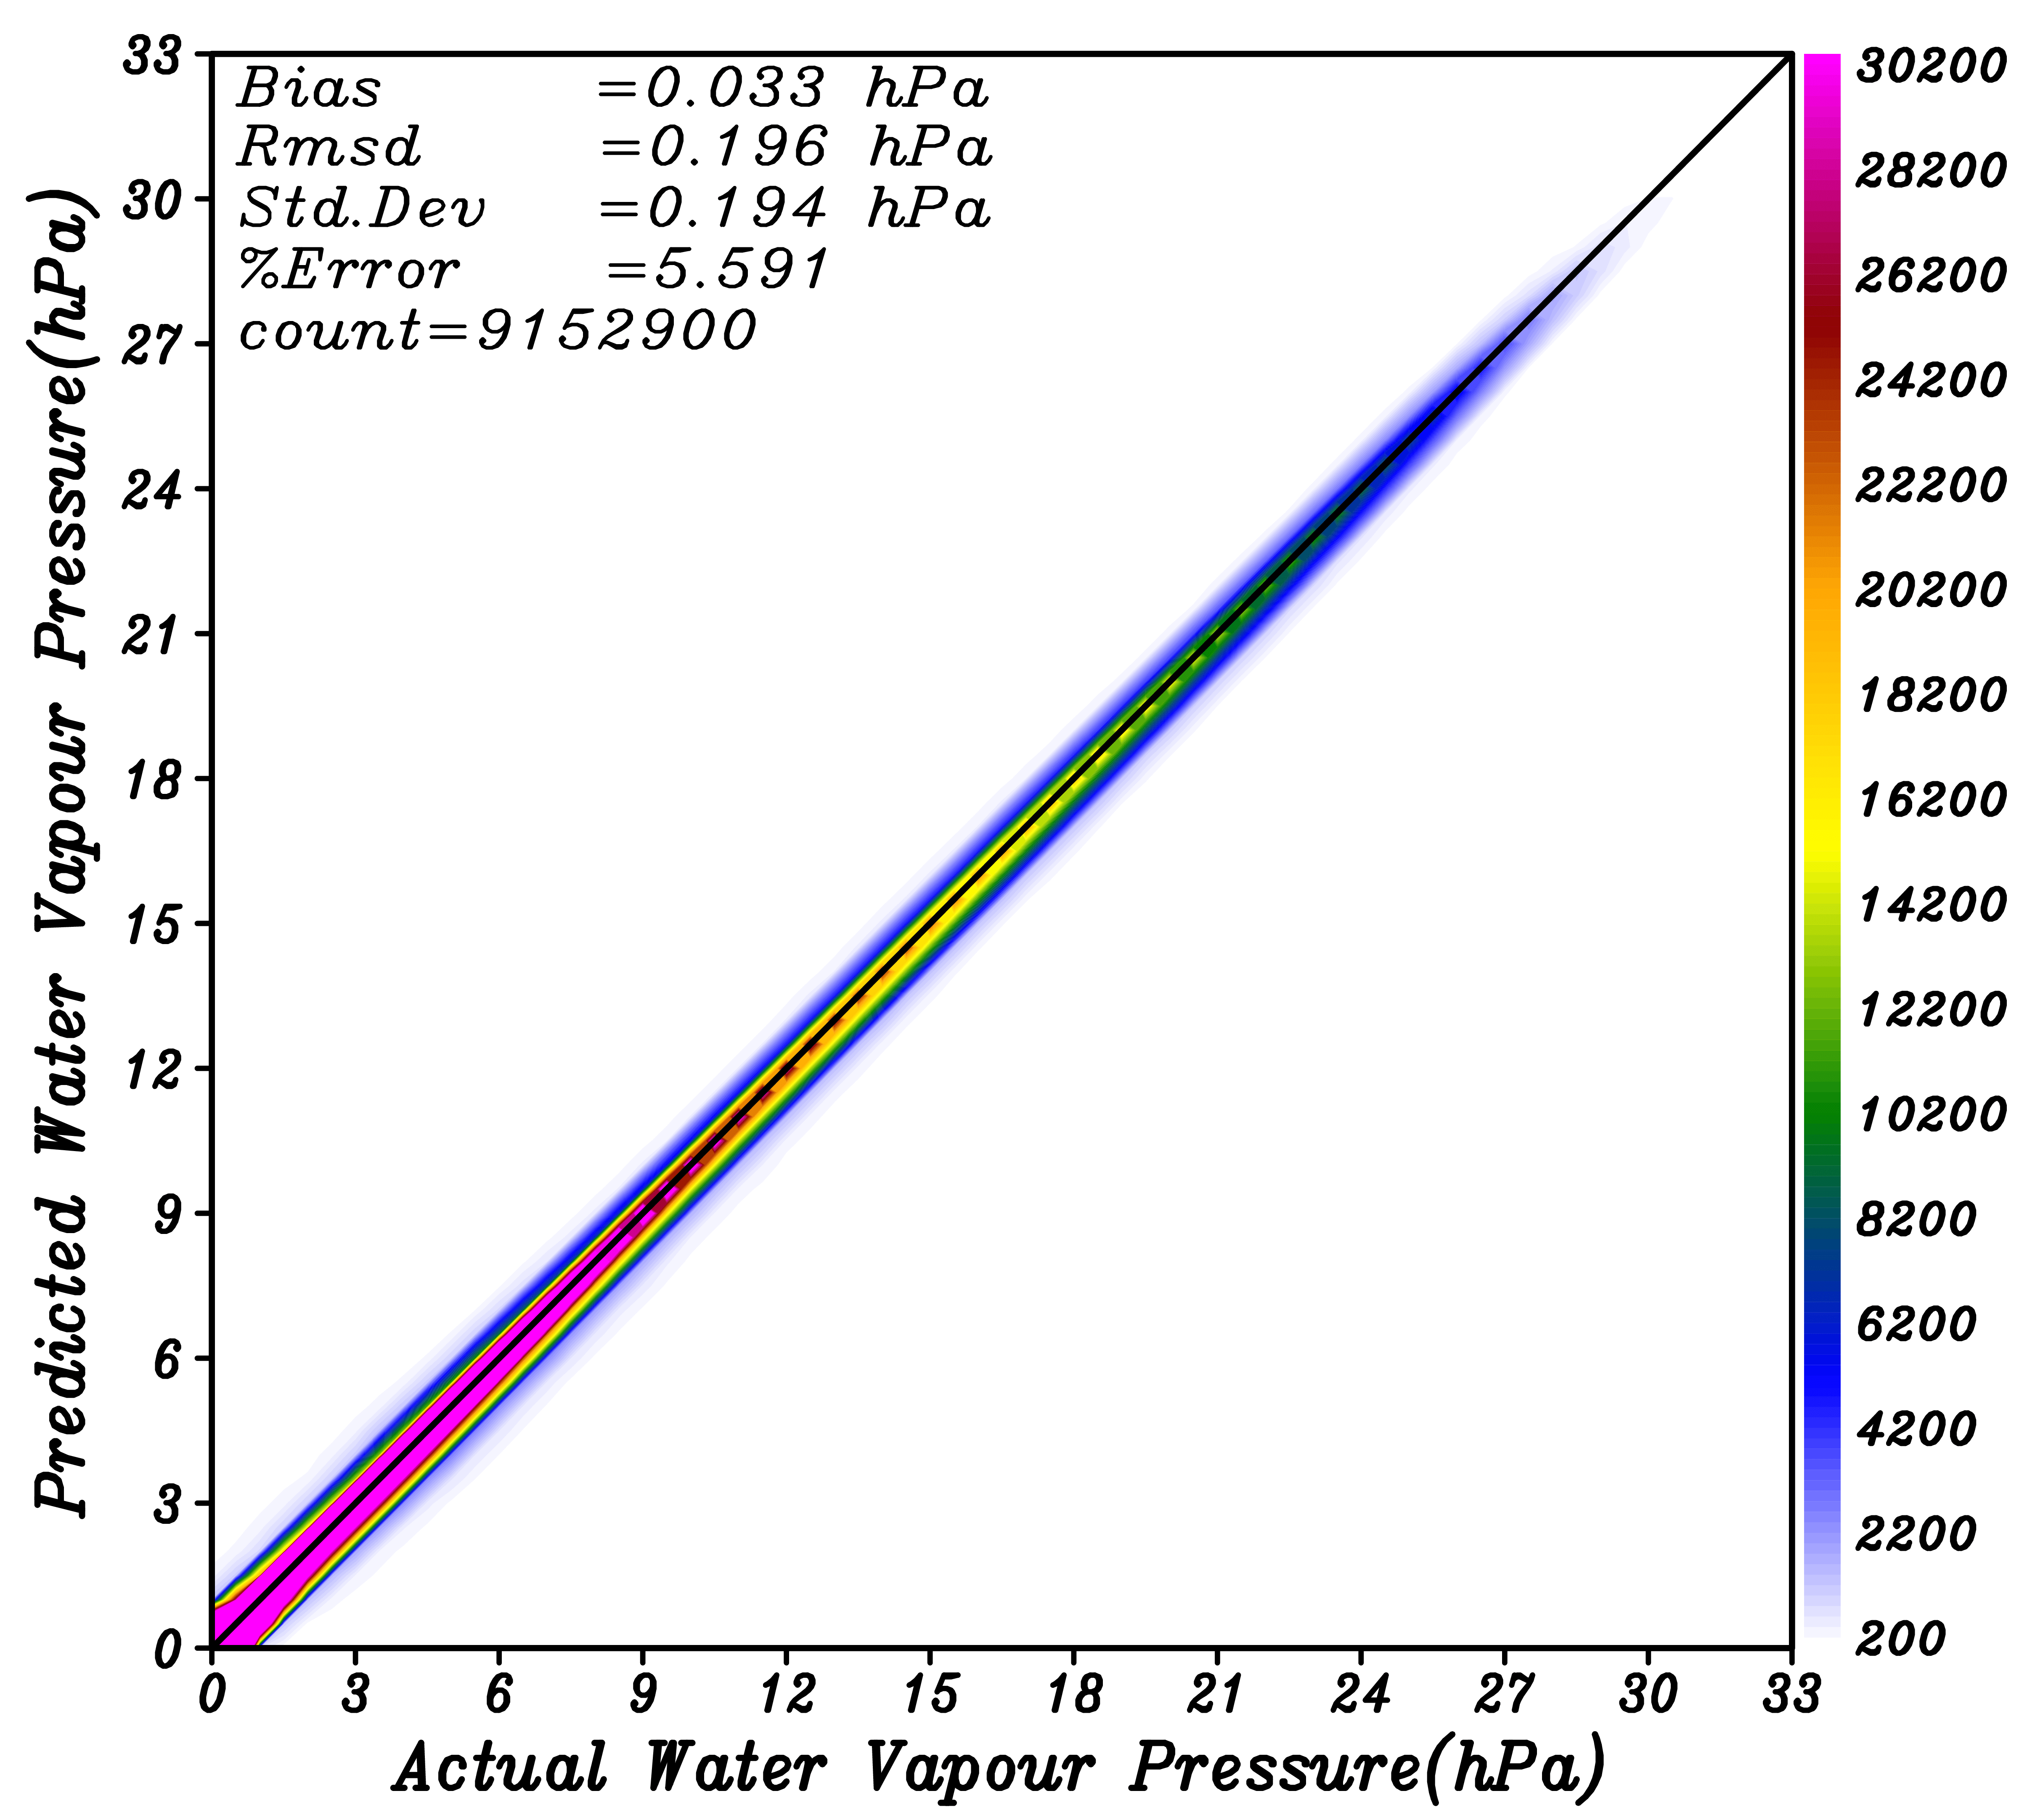
\includegraphics[width=\textwidth, height=15cm ]{images/cover-image.png}
%\caption{Scatter plot of actual versus retrieved water vapour pressure. Color bar represents the number of observations available for each water vapour pressure bin. This figure is based on data that has been accumulated over all vertical levels and the whole domain.}
%\end{figure}
%\end{center}
%------------------------------------------------
%------------------------------------------------
%------------------------------------------------
%------------------------------------------------
%------------------------------------------------
%------------------------------------------------
%------------------------------------------------
\newpage
\addcontentsline{toc}{section}{Abstract}
\tableofcontents
\listoffigures

%------------------------------------------------
%------------------------------------------------
%------------------------------------------------
%------------------------------------------------
%------------------------------------------------
%------------------------------------------------
%------------------------------------------------
\newpage
\pagestyle{fancy}
\renewcommand{\sectionmark}[1]{\markright{\thesection\,\ #1}}
%\fancyfoot[C,L,E]{} \fancyfoot[C]{\thepage} \setcounter{page}{1}
\fancyfoot[L]{\footnotesize{\it{Report: Hooda et al.}}}
\fancyfoot[R]{\footnotesize{\it{GNSS RO Atmospheric Profile Retrieval}}}
\renewcommand{\footrulewidth}{0.4pt}


%------------------------------------------------
%------------------------------------------------
%------------------------------------------------
%------------------------------------------------
%------------------------------------------------
%------------------------------------------------
%------------------------------------------------
\section{Introduction}
\noindent  Earth's atmosphere is highly nonlinear in nature, and continuous monitoring applications such as weather and climate modelling require reliable tropospheric thermodynamic profiling (i.e. temperature, moisture and pressure). Radiosonde observations are the most reliable measurements for this purpose. However, these observations are very sparse and not available over the oceans. Moreover, they have manual dependency too. Sounders onboard satellites remove this dependency and provide global observations at high spatial and temporal resolutions (\textit{Xu et al.}, 2019).\\ 


\noindent Infrared (IR) sounders can provide thermodynamic profiles in clear-sky conditions, but they have limitations during cloudy and precipitating environments. Microwave (MW) sounders improve on the IR sounders, but they are also sensitive to heavy precipitation which limits their use in extreme weather events. On the contrary, the radio occultation (RO) measurements from the Global Navigation Satellite System (GNSS) have the advantage of monitoring Earth's atmosphere in all weather conditions with high vertical resolution. RO data is minimally affected by aerosols, clouds, or precipitation, does not require calibration and is free from instrument drift and satellite-to-satellite bias (\textit{Anthes}, 2011; \textit{Anthes et al.}, 2000, 2003, 2008; \textit{Chen et al.}, 2021; \textit{Hajj et al.}, 2004; \textit{Kuo et al.}, 2004; \textit{Rocken et al.}, 1997; \textit{Wickert et al.}, 2004). These unique features make RO data ideal for weather and climate studies (\textit{Scherllin-Pirscher et al.}, 2021; \textit{Steiner et al.}, 2011). Due to the success of COSMIC-1, US agencies and Taiwan decided to move forward with a follow-on Global Navigation Satellite System Radio Occultation (GNSS-RO) mission called FORMOSAT-7/COSMIC-2. The six COSMIC-2 satellites launched successfully on June 25, 2019, into low inclination orbits. COSMIC-2 can  provide $~5000$ RO profiles over the tropics and subtropics daily (\textit{Xu et al.}, 2019). RO techniques have been successfully assimilated into numerical weather prediction models which greatly improved forecast quality (\textit{Rennie}, 2010). \\

\noindent An RO occurs when a receiver in low-Earth orbit (LEO) views a GNSS satellite as it sets or rises behind the Earth’s atmosphere. The measured signal phase and amplitude are analyzed to derive atmospheric refractivity using a limb-sounding geometry.
The atmospheric state variables such as pressure, water vapour pressure and temperature (i.e. P, e and T) can be derived from the inversion of atmospheric refractivity observations. RO observations in weather and climate modelling are used in two manners. In the first approach, the refractivity or bending angle profiles are directly assimilated in NWP models. In the second approach, thermodynamic profiles are extracted from these refractivity profiles using optimum theory-based variational methods such as the 1Dvar approach. This approach requires \emph{a priori} knowledge of the atmospheric state variables (P, e and T) which are obtained from either climatology or NWP model forecasts, the latter being the more widely used. There is redundancy and dependency in this method, as retrieval requires external data sources which introduces lag for real-time application. The use of \emph{a priori} can be avoided by developing an empirical relationship between the atmospheric state variables and the RO refractivity observations using a collection of a large dataset (\textit{Leroy et al.}, 2012). \\

\noindent Machine learning (ML) has seen a recent surge in earth-atmosphere applications due to its immense prowess. ML consists of algorithms that learn and establish relationships among the dependent and independent variables from a collection of datasets. Training an ML algorithm is a one-time process but is computationally expensive. As high-speed computers are readily available nowadays, the application of ML algorithms has become ubiquitous. Deep learning is a subfield of ML based on neural networks, which are highly flexible differentiable functions that can be fit to data to help learn factors of variation that explain the observed data. Neural networks consist of a hierarchy of layers that contain nodes performing weighted non-linear transformations of their inputs, through a series of hidden layers, to the desired output. Deep learning solves the central problem in representation learning by introducing representations expressed in terms of other, simpler representations. Deep learning allows the computer to build complex concepts out of simpler concepts (\textit{Goodfellow et al.}, 2016).\\ 

\noindent  This study aims to develop a deep learning-based algorithm to reduce continuous dependency on meteorological information from external sources while deriving thermodynamic profiles from RO refractivity observations. The structure of the document is as follows, section 2 discusses the GNSS RO-based  technique, section 3 discusses the data and methods used, section 4 discusses the results and section 5 provides the conclusion.\\

\section{GNSS RO Technique}

\noindent The basic principle of the GNSS RO technique is the interaction between electromagnetic radiation and a medium i.e., in this case the terrestrial atmosphere using a limb-sounding geometry. As the signals propagate from the GNSS satellite to the receiver on the LEO satellite, they are delayed (due to bending as well as retardation) by the ionosphere and the neutral atmosphere (\textit{Davis et al.}, 1985). The ionospheric delay is frequency dependent which can be cancelled using two different frequencies to obtain ionospheric free measurements. The tropospheric neutral atmosphere delay is directly proportional to the refractive index or refractivity and can be expressed as a function of atmospheric temperature, pressure and water vapour pressure. \\

\noindent Figure \ref{fig:img30} schematically illustrates the geometry of the GNSS-LEO occultation of the Earth's atmosphere in the occultation plane. The overall effect of the atmosphere can be characterized by a total bending angle ($\alpha$) as a function of the impact parameter ($a$). The impact parameter is defined, assuming spherical symmetry, as the perpendicular distance between the centre of the Earth (more precisely speaking, the centre of local curvature at the perigee of the occultation ray) and the ray asymptote at the GNSS or LEO satellite. The variations of $\alpha$ with $a$ or $r$ (radius to ray tangent point) depend primary on the vertical profile of the atmospheric refractive index. \\

\begin{figure}[H]
\centering
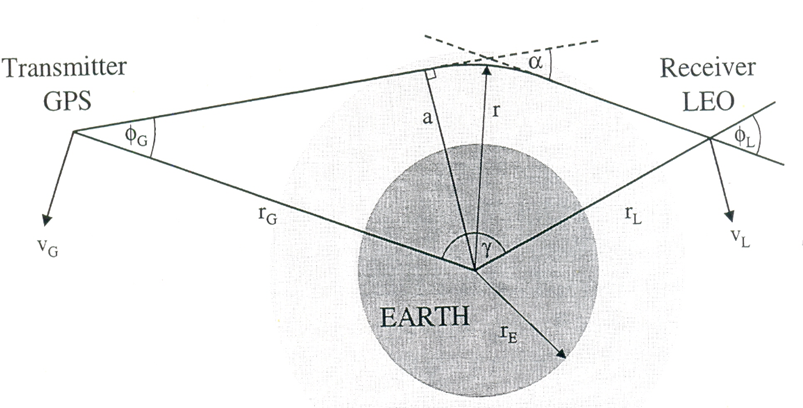
\includegraphics[width=\textwidth, height=8cm , frame]{images/Figure19.png}
\caption{Conceptual sketch showing the geometry of the GNSS-LEO occultation of the Earth's atmosphere in the occultation plane. The GNSS satellite (radius vector $r_{G}$, velocity $v_{G}$) emit rays at the zenith angle $\phi_{G}$, which are received by the LEO satellite (radius vector $r_{L}$, velocity $v_{L}$) at the zenith angle $\phi_{L}$. The total bending angle is denoted by $\alpha$ and radius at the tangent point r.}
\label{fig:img30}
\end{figure}

\noindent Refractivity profile can be retrieved from measurements of $\alpha(a)$ during occultations assuming local spherical symmetry. In the case of the radio frequency domain, accurate angular measurements are difficult to achieve since they would require a very large dimension of the receiving antenna (\textit{Gorbunov and Sokolovkiy}, 1993). Instead, it is possible to measure the phase (or Doppler frequency) shift of the signal with extremely large accuracy as a function of time. These measured phase paths include both the geometric paths from the transmitter to the receiver and the optical path due to atmospheric bending. By derivation of the signal phase with respect to time, the Doppler shifted frequency is calculated. The residual Doppler shift due to atmospheric bending can be combined with satellite position and velocity knowledge to estimate the bending angle and impact parameter. This gives a set of $\alpha$($a$) which has to be inverted into a vertical profile of  refractivity close to the tangent point. Assuming that the set of tangent points are not significantly separated in the horizontal and that the atmosphere can be approximated locally as spherically symmetric, there is a direct solution to the inverse problem through an Abel transform. \\

\subsection{Atmospheric bending and the inverse refractive problem}

\noindent \textit{Phinney and Anderson} (1968) deduced inversion relation for the determination of refractive index profiles from either the phase shift or the angular path. With the geometric optics assumption for the propagation of electromagnetic signals, the path of a ray through a region of varying refractive index is determined globally by Fermat’s principle of least time. Thus, the trajectory of the electromagnetic ray connecting two points (P1, P2) can be obtained through setting.
\begin{equation}
	\int _{p1}^{p2}nds=Min\
\end{equation}
It is evident that it is not possible to retrieve the three dimensional variation of the refractive field in the vicinity of the ray perigee from the one dimensional measurements along the trajectory of the receiving satellite. A simplification of the problem has to be made in which it can be considered as the horizontal displacement of the transmitting ray perigee crossing the atmosphere to be much smaller than the characteristic horizontal scale of meteorological fields (\textit{Gorbunov and Sokolovskiy}, 1993). This can make the approximation that the ray path is lying in a plane. Furthermore, it was shown by \textit{Lusignan et al.} (1969) that the horizontal component of the refractive index gradient normal to the ray path may be ignored since it causes negligible small errors to angular and Doppler data. The variation of $n$ along the limb path is dominated by the vertical gradient of the refractive index field. This gradient of n is directed radially by making the assumption that the local refractive index field is distributed spherically symmetrical in the vicinity of the ray perigee. For the ray changing its direction when passing through the refractive index field, basically Snell's law (\textit{Born and Wolf}, 1980) may be applied
\begin{equation}
	nsin\phi=const 
\end{equation}
\noindent where $\phi$ denotes the angle between the gradient of refraction and the ray path. If the ray path lies in one plane, then the change in direction can be expressed in polar coordinates.

\noindent The differentiation of Snell's law $dn\sin\phi + n\cos\phi d\phi=0$ leads to the equation for the incremental bending of the ray, which can be rearranged as:
\begin{equation}
	d\alpha =d\phi _{snell} =-\tan \phi \frac{dn}{n} 
\end{equation}
The angle of incidence $\phi $  is related to the polar coordinate in that
\begin{equation}
	\tan \phi =\frac{rd\theta }{dr}
\end{equation}
Since Snell's law is defined for planner interfaces the total change in the incremental angle $d\phi $ has two contributions, the one described by Snell's law $\left(d\phi _{snell} \right)$ plus an additional contribution due to the spherically symmetric interfaces, and thus the change of the incident angle with respect to the change of the polar angle $\frac{\partial \phi }{\partial \theta } \, d\theta$ (\textit{Kursinski}, 1997). Using the geometrical relation $\theta +\phi -\alpha ={\raise0.7ex\hbox{$ \pi  $}\!\mathord{\left/{\vphantom{\pi  2}}\right.\kern-\nulldelimiterspace}\!\lower0.7ex\hbox{$ 2 $}} $ with its differential form
\begin{equation}
	d\theta +d\phi - d\alpha =0 
\end{equation}
And substituting for $d\theta$ and $d\phi$ by using Eq. 3 and Eq. 4gives
\begin{equation}
	\frac{dn}{n} +\frac{dr}{r} +\frac{d\phi }{\tan \phi } =0 
\end{equation}
Integration of Eq. 6 leads to the formula of Bouguers ()\textit{Born and Wolf}, 1980) which represents the equation for the ray trajectory in a spherically symmetrical refractive field and replaces Snell's law for a plane stratified medium:
\begin{equation}
	nr\sin\phi =cont=a 
\end{equation}                                   
\noindent The quantity $r\sin \phi$ represents the perpendicular distance from the origin to the ray path tangent. As $ r$  goes to infinity, $n$ goes to unity, so that the constant term must equal the impact parameter (a). At the point of closet approach, denoted by the ray tangent radius $r_{o} \sin\phi =1$. So that a=n (r${}_{0}$) r${}_{0.}$ \\

\noindent In order to derive the total refractive bending angle, the Bouguer equation is rearranged to get $\sin\phi ={\raise0.7ex\hbox{$ a $}\!\mathord{\left/{\vphantom{a nr}}\right.\kern-\nulldelimiterspace}\!\lower0.7ex\hbox{$ nr $}} $ which substitute for tan$\phi $ in Eq.6. Integration along the ray path then gives the integral equation

\begin{equation}
	\alpha \left(a\right)=2a\int _{r=r_{0} }^{r=\infty }\frac{1}{\sqrt{n^{2} r^{2} -a^{2} } }  \frac{d\ln (n)}{dr} dr
\end{equation}
This so called Abelian integral equation addresses the forward calculation of \textit{$\alpha$(a)} from a given \textit{n(a).} The equation has to be inverted employing standard mathematical techniques, i.e., using the Abelian transformation to retrieve the refractive index as a function of the tangent 
\begin{equation}
	n\left(r_{0} \right)=\exp \, \left[\frac{1}{\pi } \int _{a=\infty }^{a=a_{0} }\frac{\alpha \left(a\right)}{\sqrt{a^{2} } -a_{0}^{2} }  da\right]
\end{equation}
Here the impact parameter `\textit{a'} corresponds to the radius at the tangent point $r_{0} =n(r)/a_{0}$ for the ray of closest approach. This equation describes a set of rays in that \textit{da} is being integrated from a${}_{0}$ to infinity using the measurements of $\alpha$(a). In practice a discrete approach with a numerical solution is performed. A description of the derivation of the Abelian integral equation and its solution with respect to n(r) leading to the Abelian integral transform pair was given by \textit{Fjeldbo et al.} (1971). 

\subsection{Derivation of the bending angle from phase measurements}

\noindent In the radio frequency domain, the effect of atmospheric bending can be measured as phase $(\phi)$ delays or excess phase $(\nabla \phi)$ for the GNSS signal paths due to the slowing and bending of both the atmosphere and ionosphere. From these observables, computed excess phase paths (L) and Doppler shifts (dL/dt) can be combined with satellite position and velocity vectors measurements to determine the atmospheric bending angle. In the following, the standard methodology for the derivation of bending angles from phase measurements is described.\\

\noindent The excess phase paths (L${}_{1}$ and L${}_{2}$) for the dual frequency GNSS signals obey the following relation:  
\begin{equation}
	L_{i} =\Delta \phi _{i}\lambda _{i} =\int n\left(s_{i} \right) ds_{i} -R_{geom}
\end{equation}
where R${}_{geom}$ denotes the geometrical straight line distance (vacuum path length) between the receiver and transmitter, and $\lambda$ is the wavelength of the probing signal. The rays of the two GNSS frequencies f${}_{1}$ and f${}_{2}$ are influenced differently by the ionosphere because of its dispersive properties and travel along different paths. Since the main interest is refractive index of the neutral atmosphere, the contribution of the ionospheric bending in the excess phase path has to be removed by applying an ionospheric correction method. For the standard ionospheric correction method, a linear combination of the excess phase paths of the two signals with harmonically related frequencies is performed:
\begin{equation}
	L_{c} =\frac{f_{1}^{2} L_{1} -f_{1}^{2} L_{2} }{f_{1}^{2} -f_{2}^{2} } 
\end{equation}
This is a model correction of the ionospheric optical path length, removing contributions up to the first order. The excess phase path L${}_{c}$ now consists only of the delay due to the neutral atmospheric bending plus a small ionospheric residual, i.e., the higher order terms. The derivation of L with respect to time (dL${}_{c}$/dt) then gives the atmospheric Doppler shift f${}_{d}$ on the carrier frequency f which can be related to kinematic properties such that
\begin{equation}
	\frac{f_{d} }{f} c=\frac{dL_{c} }{dt} =v_{G}^{c} \sin \phi _{G} -v_{L}^{c} \sin \phi _{L} +v_{G}^{c} \cos \phi _{G} +v_{L}^{c} \cos\phi _{L} 
\end{equation}
The GNSS satellite emits electromagnetic waves at zenith angle $\phi _{G}$ and the signal is received at the LEO satellite at the zenith angle $\phi _{L} $. With the assumption of local spherical symmetry and the use of Snell's law of the form $r_{G} \, \sin \, \phi _{G} =r_{L\, } \sin \, \phi _{L} $, where r${}_{G}$ and r${}_{L}$ are the geocentric distances of the satellites, n(r${}_{G}$)=n(r${}_{L}$)=1 is valid. \\

\noindent By expressing $\phi _{G}$ through Snell's law and combining it with Eq. 12 the ray zenith angle at the GNSS satellite and in analogues from the ray zenith angle at the LEO satellite is derived with the known position and velocities of the satellites. Finally the atmospheric bending angle and the ray parameters can be calculated with the knowledge of the angle $\gamma$ from the satellite positions:

\begin{equation}
	\alpha \left(a\right)=\phi _{G} +\phi _{L} +\gamma -\pi
\end{equation}
\begin{equation}
	a=r_{G}^{} \sin \phi _{G} =r_{L}^{} \sin \phi 
\end{equation}

\subsection{Atmospheric property derivation from the refractive index}

The total ionospheric and atmospheric refractivity (N) can be approximated for waves in the radio frequency domain ($\mathrm{<}$10 GHz) by:
\begin{equation}
	N=77.6890\, \frac{P}{T} -6.3938\, \frac{e}{T } +3.75463\times 10^{5} \, \frac{e}{T^{2} } +\, 4.04\times 10^{7} \, \, \frac{n_{e} }{f^{2} } 
\end{equation}
where $P$ denotes the pressure (mb), $T$ is the atmospheric temperature in (K), $e$ is water vapour partial pressure in (mb), $n_{e}$ is the electron number density in (m${}^{-3}$), and $f$ denotes the transmitter frequency in (Hz). Three main sources, the dry neutral atmosphere, water vapour, and free electrons in the ionosphere contribute to the total refractivity in Eq. 15. Further, scattering from large rain drops is neglected in Eq. 15, as it is important only under very extreme conditions.\\

\noindent The first term in Eq. 15 is due to the dry part of the atmosphere. This dry term is caused by the polarizability of molecules in the atmosphere which means that the incident electric field induces an electric dipole in the molecule. The dry refractivity term is proportional to the molecular number density and dominates in altitudes from the surface up to about 50 km. The second and third terms, represent the wet part of the refractivity which is due to the large permanent dipole moment of water vapour. Throughout most of the troposphere, the dipole component of the refractivity is about 20 times larger than the non-dipole component (\textit{Bevis et al.}, 1992). The moist terms have only a substantial impact on the magnitude of $ N$ in the lower troposphere, i.e., below 5 km, above altitudes of 7 to 10 km, the contribution to $N$ from the water vapour terms is less than 2\%.\\

\noindent The fourth term, the ionospheric term, is mainly due to free electrons in the ionosphere and becomes important above about 50 km. This term is proportional to the free electron number density and is an approximation of the Appleton-Hartee equation, which represents the full dispersion relation for ionised plasma. The dispersive nature of the ionosphere causes the ionospheric term to depend on the frequency. This term is estimated and removed to first order combination of the two frequency GNSS measurements to derive the neutral atmospheric refractivity. Removing the ionospheric term leaves the dry and the moist term which represents then the equation for neutral refractivity. This equation is valid for the radio frequency domain and provides an accuracy of approximation 0.5 \% in $N$ (\textit{Smith and Weintraub}, 1953). \textit{Thayer} (1974) improved the equation for the radio refractive index of air by taking into account the compressibility factor due to non-ideal gas behaviour.\\

\noindent It is clear from Eq. 15 that, after accounting for the ionospheric component, it contains three unknowns (P, T and e), which makes  it challenging to retrieve thermodynamic profiles from known refractivity measurements. In the upper atmosphere where moisture content is low or negligible the hydrostatic equation and the equation of state can be used to retrieve the temperature and pressure from refractivity measurement by neglecting the moist terms in Eq. 15. The profiles  are known as dry retrievals, and are very accurate in the upper troposphere and above. However, when the water vapour content is significant, which is the case in the warmer regions of the troposphere, particularly in tropical regions where the abundance is greatest, the separate contributions to refractivity by the dry and moist terms cannot be distinguished uniquely through radio occultation measurements. This introduces an ambiguity into the profiles of water vapour pressure, pressure and temperature. In this case, the use of a priori data from meteorological analyses is necessary and is a constraint to the retrieval problem. \\

\section{Data and Methods}

\subsection{Data used}

\noindent In the present study the wetPf2 level 2 product which is available at the COSMIC Data Analysis and Archive Center (CDAAC) website (https://data.cosmic.ucar.edu/gnss-ro/cosmic2/nrt/level2/) was used. The product contains meteorological profiles of temperature, pressure and water vapour pressure with a vertical resolution of 50 m from surface to 30 km height and a vertical resolution of 200 m from 30 km to 60 km height, derived from COSMIC-2 measured refractivity using the 1DVar approach with European Centre for Medium-Range Weather Forecasts (ECMWF) 6 hour forecasts as the prior (or first guess) information. These thermodynamic profiles along with their respective spatial and temporal metadata were collected. These profiles were extracted for the Indian subcontinent (Latitude: 45$^\circ$E to 110$^\circ$E, Longitude: 0$^\circ$N to 45$^\circ$N) in the January 2020 - December 2021 time period. Note that the CDAAC profiles incorporate refractivity as well, computed using the 2-term refractivity formulation, and is compatible with these thermodynamic profiles (Equation 10 of Smith and Weintraub, 1953). However, recent literature showed that the 3-term refractivity formulation (\textit{Singh et al.}, 2021) performs better than the 2-term refractivity formulation therefore we have recomputed refractivity from the CDAAC thermodynamic profiles using 3-term refractivity formulation. These refractivity profiles along with the spatial and temporal metadata such as latitude-longitude, height and month-day-hour formed the independent variables. Thermodynamic profiles, temperature, pressure and water vapour pressure were the dependent variables. Note that, in this study, we have limited our analysis from surface to 15 km height only because the water vapour is negligible above 15 km altitude. Thus above 15 km the dry retrievals can be accurately performed using COSMIC-2 observed refractivity. Further note that although the original data was accessible every 50 m in the vertical, it was decided to take the data at a 100 m vertical  resolution to develop and test the model. Also note, that the study excludes the highly mountainuous regions (regions higher than 1 km) as the quality of data there is unknown. \\


\noindent In order to choose the most ideal number of independent parameters for the model development, we performed a correlation study between the dependent and independent variables. Figure \ref{fig:img5} shows the correlation between these independent and dependent variables. The association between refractivity and moisture (e.g., water vapour pressure) is significant in the lower troposphere, whereas in the upper troposphere, the correlation between refractivity and pressure (P) is stronger than the correlation with water vapour pressure. The association between refractivity and temperature is much weaker than it is for pressure (P) and water vapour pressure (e). Overall, it can be observed that the association between refractivity and total pressure increases as height increases, whereas the correlation between refractivity and water vapour pressure drops. As would be expected, temperature, pressure, and water vapour pressure all negatively correlate with height, with pressure and height having a much stronger correlation. \\

\noindent Except for higher level temperature, which has a positive link with latitude, the majority of variables have negative correlations with latitude. Furthermore, the relationship between pressure and latitude is weaker in the lower troposphere and stronger in the upper troposphere. As one moves from the tropics to higher latitudes, both water vapour pressure and temperature decrease, so it makes sense that there is a negative correlation between latitude and water vapour pressure. The relationship between pressure and latitude, however, is not simple and depends on the dynamics and thermodynamics of various atmospheric processes in a very complex way. Also, longitude and the month have a positive correlation with water vapour pressure across the entire height. While less significant than the association between water vapour pressure and longitude and month, the correlation between temperature and longitude appears to be strongly positive in the middle troposphere and negative in the upper troposphere.  The total pressure has a weak positive association with longitude and months, in contrast to water vapour pressure and temperature, and is primarily observed in the upper troposphere. Day and hour correlations with all of the dependent variables are quite weak when compared to other independent variables. Therefore the independent variables day and hour were subsequently dropped during feature selection owing to their low correlation. Therefore, our model independent feature set after correlation analysis consisted of refractivity, latitude, longitude, height and month, which is unlike the feature set used by \textit{Lasota} (2021), where hour was considered to be a useful feature and longitude was not while setting up the training procedure for retrieval of profiles at the global scale. We attribute this difference to the variability observed over the Indian subcontinent. \\

	\begin{figure}[H]
		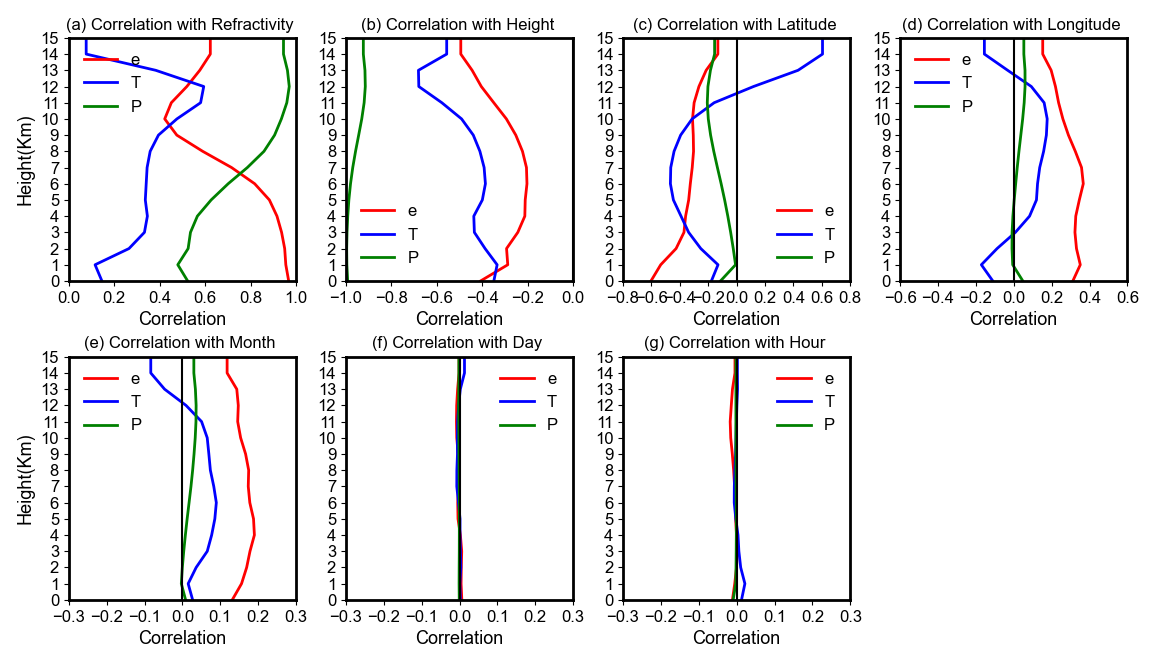
\includegraphics[width=\linewidth, height=10cm]{/Users/soumilhooda/Desktop/COSMIC_REPORT/NEW-FIGURES/Figure_corr.png}
		\caption{Correlation between dependent and independent variables using the data available within the chosen region (0$^\circ$N-45$^\circ$N, 45$^\circ$E-110$^\circ$E). The correlation is carried out for varous heights ranging from the surface to 15 km.}
		\label{fig:img5}
	\end{figure}

\noindent  The model was trained using data from the year 2020. Thirty per cent of the data from the year 2020 was utilized for testing (Test20) and seventy per cent of the data from the year 2020 was used for training (Train20) the model. Further, along with the 2020 test data set, the entire 2021 data set (Test21) was employed as an entirely independent test to check the efficiency of the developed model. The climatological variability of the three targets has been plotted in Figure \ref{fig:img2}, \ref{fig:img3} and \ref{fig:img4}.  Figure \ref{fig:img9} denotes the sample count for different heights used in the study, and Figure \ref{fig:img22} shows the same spatially. Since COSMIC-2 is in a low-inclined orbit, as was already mentioned, the amount of data counts appears to be higher around the equator and decreases as we approach higher latitudes. Nevertheless, there are still enough data counts accessible from all the locations, with a noteworthy decrease in the number of counts over a few isolated areas in the domain's northern region. The variability of the derived refractivity observations has been plotted in Figure \ref{fig:img8}. For the minimum, mean and maximum values, respectively, the water vapour pressure at the surface ranges between 0.154 hPa, 20.403 hPa and 34.656 hPa. The mean values range between 20.403 hPa at the surface and 0.002 hPa at the height of 15 km, with standard deviations of roughly 6.106 hPa at the surface and 0.0015 hPa at the height of 15 km. The minimum, mean and maximum values of the surface temperature are 252 K, 295 K and 322 K, respectively. The standard deviation spans from 2.6 K to 5 K, while the mean values vary from 295 K at the surface to roughly 207 K at 15 km. The surface pressures are 920 hPa, 995 hPa and 1036 hPa for the minimum, mean and maximum, respectively. The mean values range from 945 hPa at the surface to approximately 145 hPa at the height of 15 km, with a standard deviation that varies from 13 hPa at the surface to almost 2 hPa at the height of 15 km. Overall, it appears that both training and testing data sets have similar distributions of all the data. For the minimum, mean and maximum values, respectively, the refractivity at the surface ranges between 235, 335 and 400. The mean values range from 335 at the surface to around 55 at the height of 15 km, with standard deviations of about 28 at the surface and 3 at the height of 15 km. \\

\begin{figure}[H]
	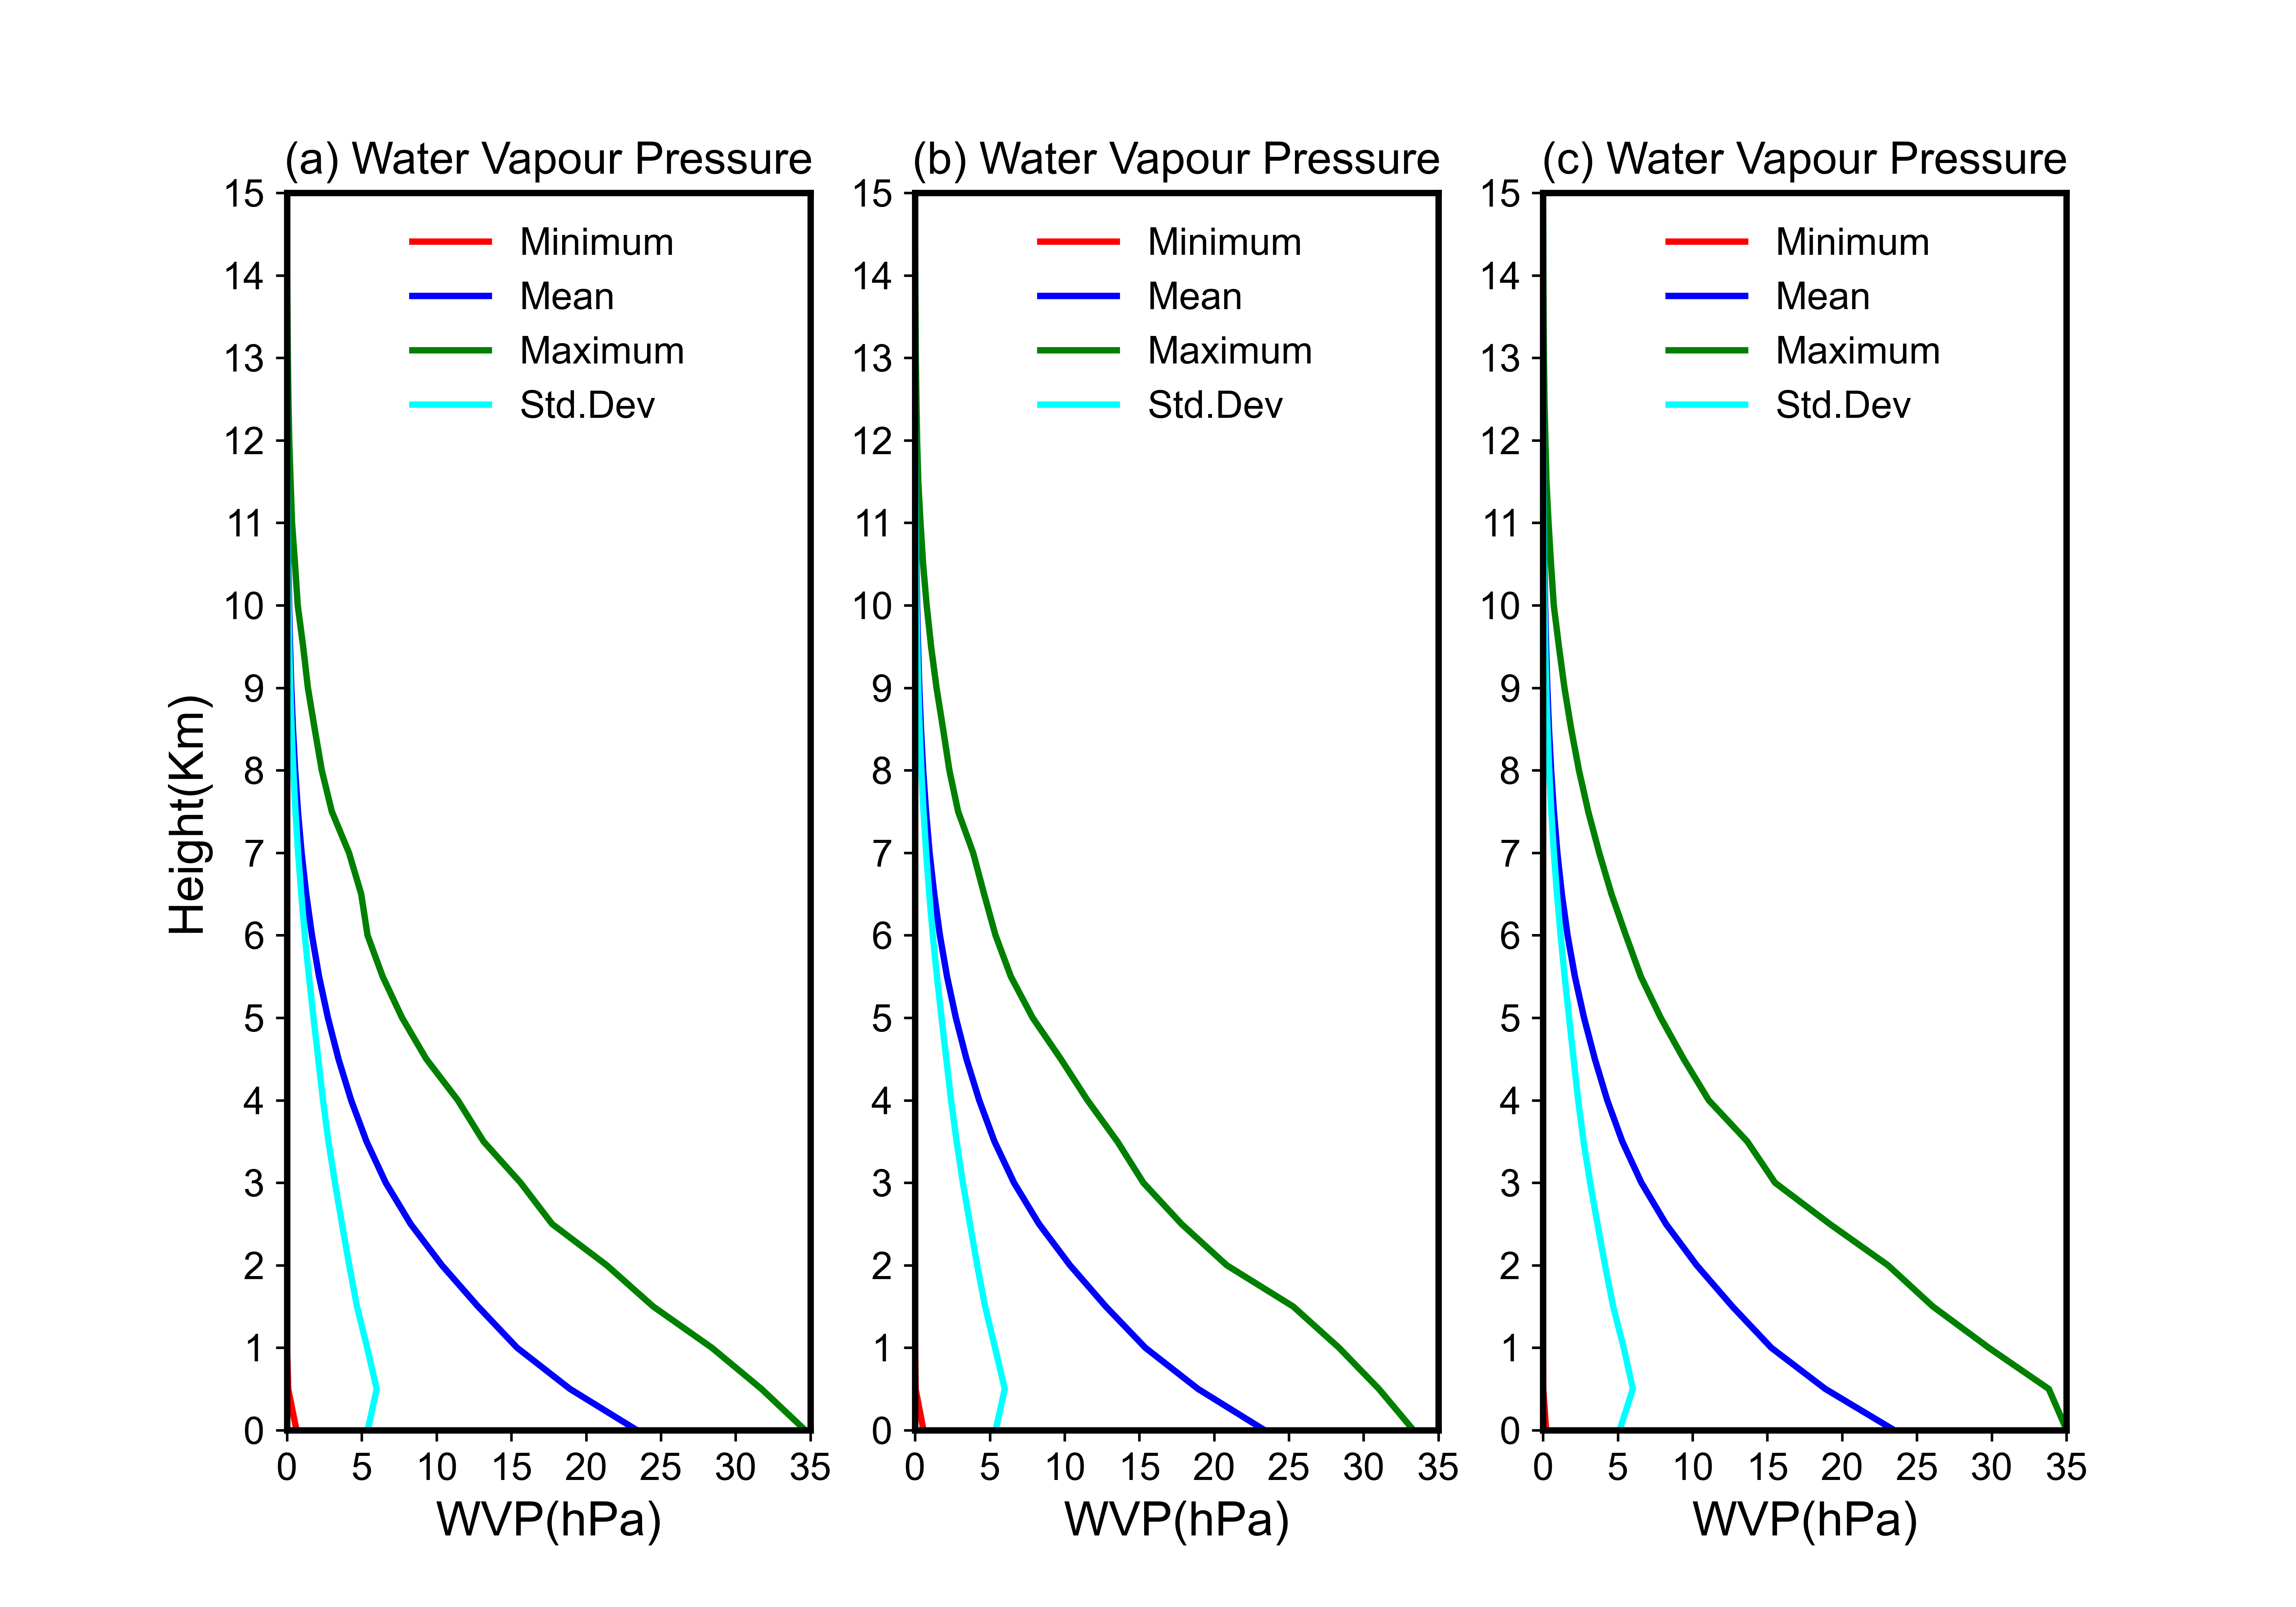
\includegraphics[width=14cm, height=8cm ]{/Users/soumilhooda/Desktop/COSMIC_REPORT/NEW-FIGURES/evp-min-mean-max-std-stats-profile.png}
	\caption{Statistical analysis of water vapour pressure data obtained from wetPf2. Leftmost panel indicates the training data from 2020, middle panel is the testing data from 2020, rightmost panel indicates the testing data from 2021. }
	\label{fig:img2}
\end{figure}
\begin{figure}[H]
	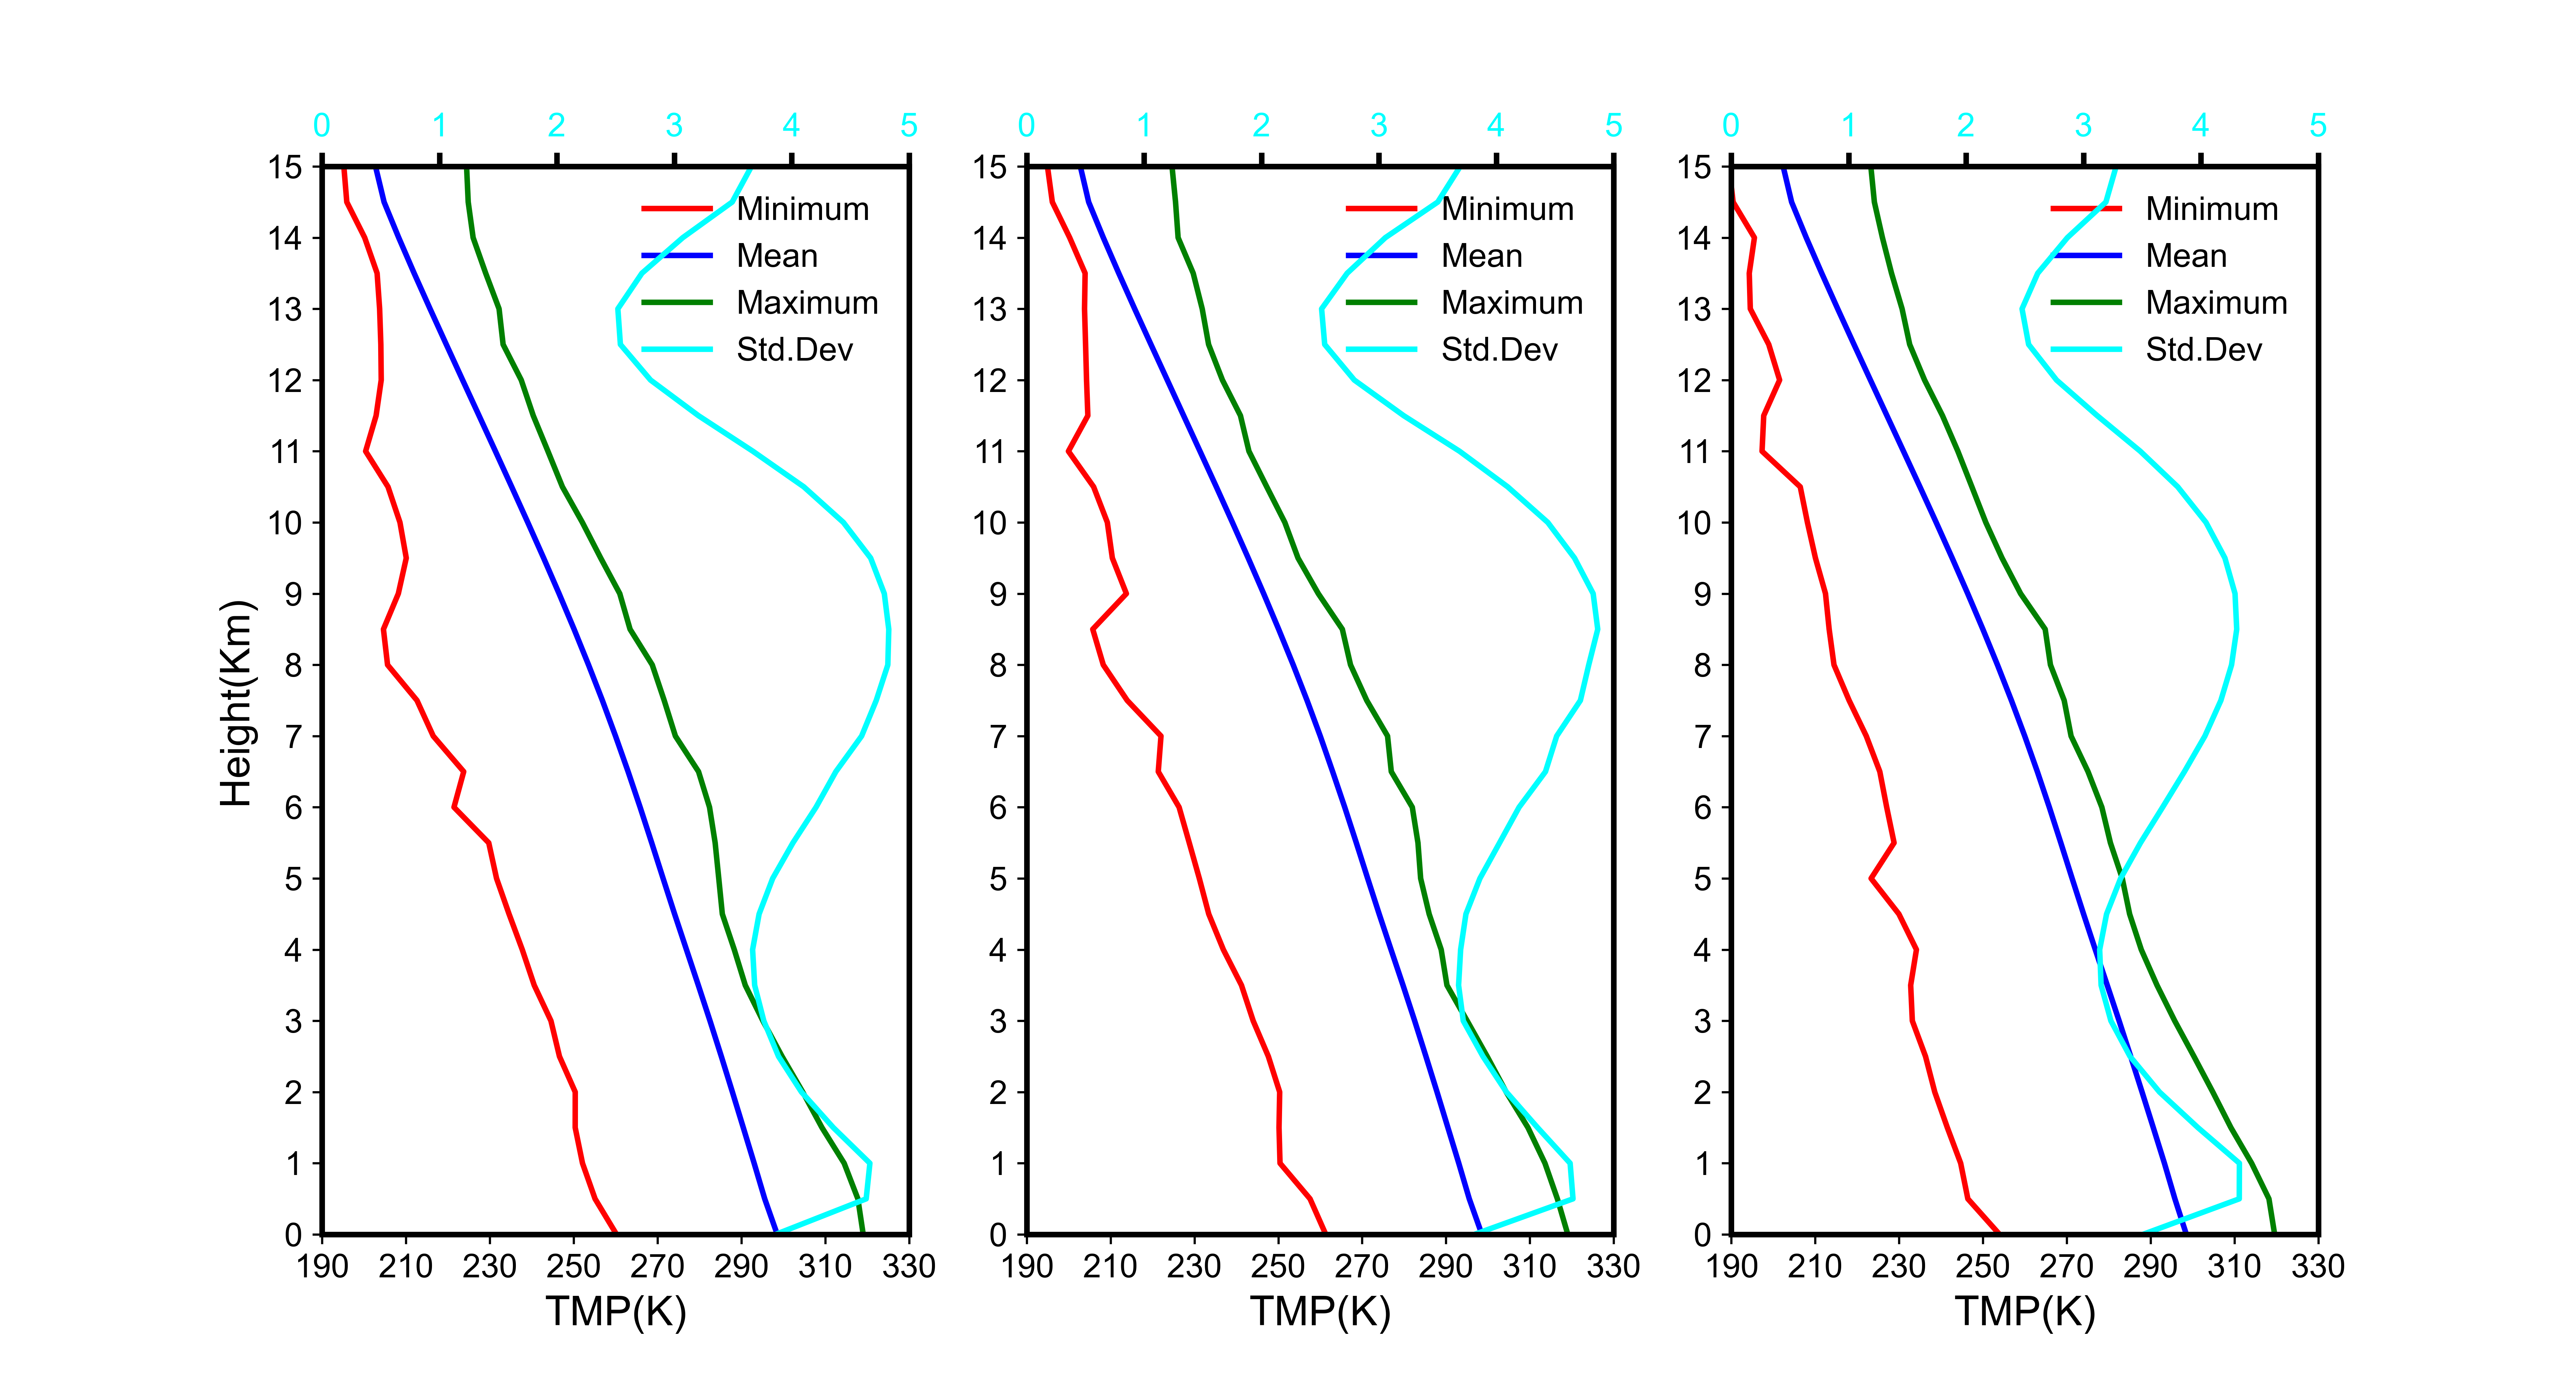
\includegraphics[width=14cm, height=8cm]{/Users/soumilhooda/Desktop/COSMIC_REPORT/NEW-FIGURES/tmp-min-mean-max-std-stats-profile.png}
	\caption{Statistical analysis of temperature data obtained from wetPf2. Leftmost panel indicates the training data from 2020, middle panel is the testing data from 2020, rightmost panel indicates the testing data from 2021. The top x axis is used to plot the standard deviation scale. The points accumulated over the entire domain are used to generate these statistics.}
	\label{fig:img3}
\end{figure}
\begin{figure}[H]
	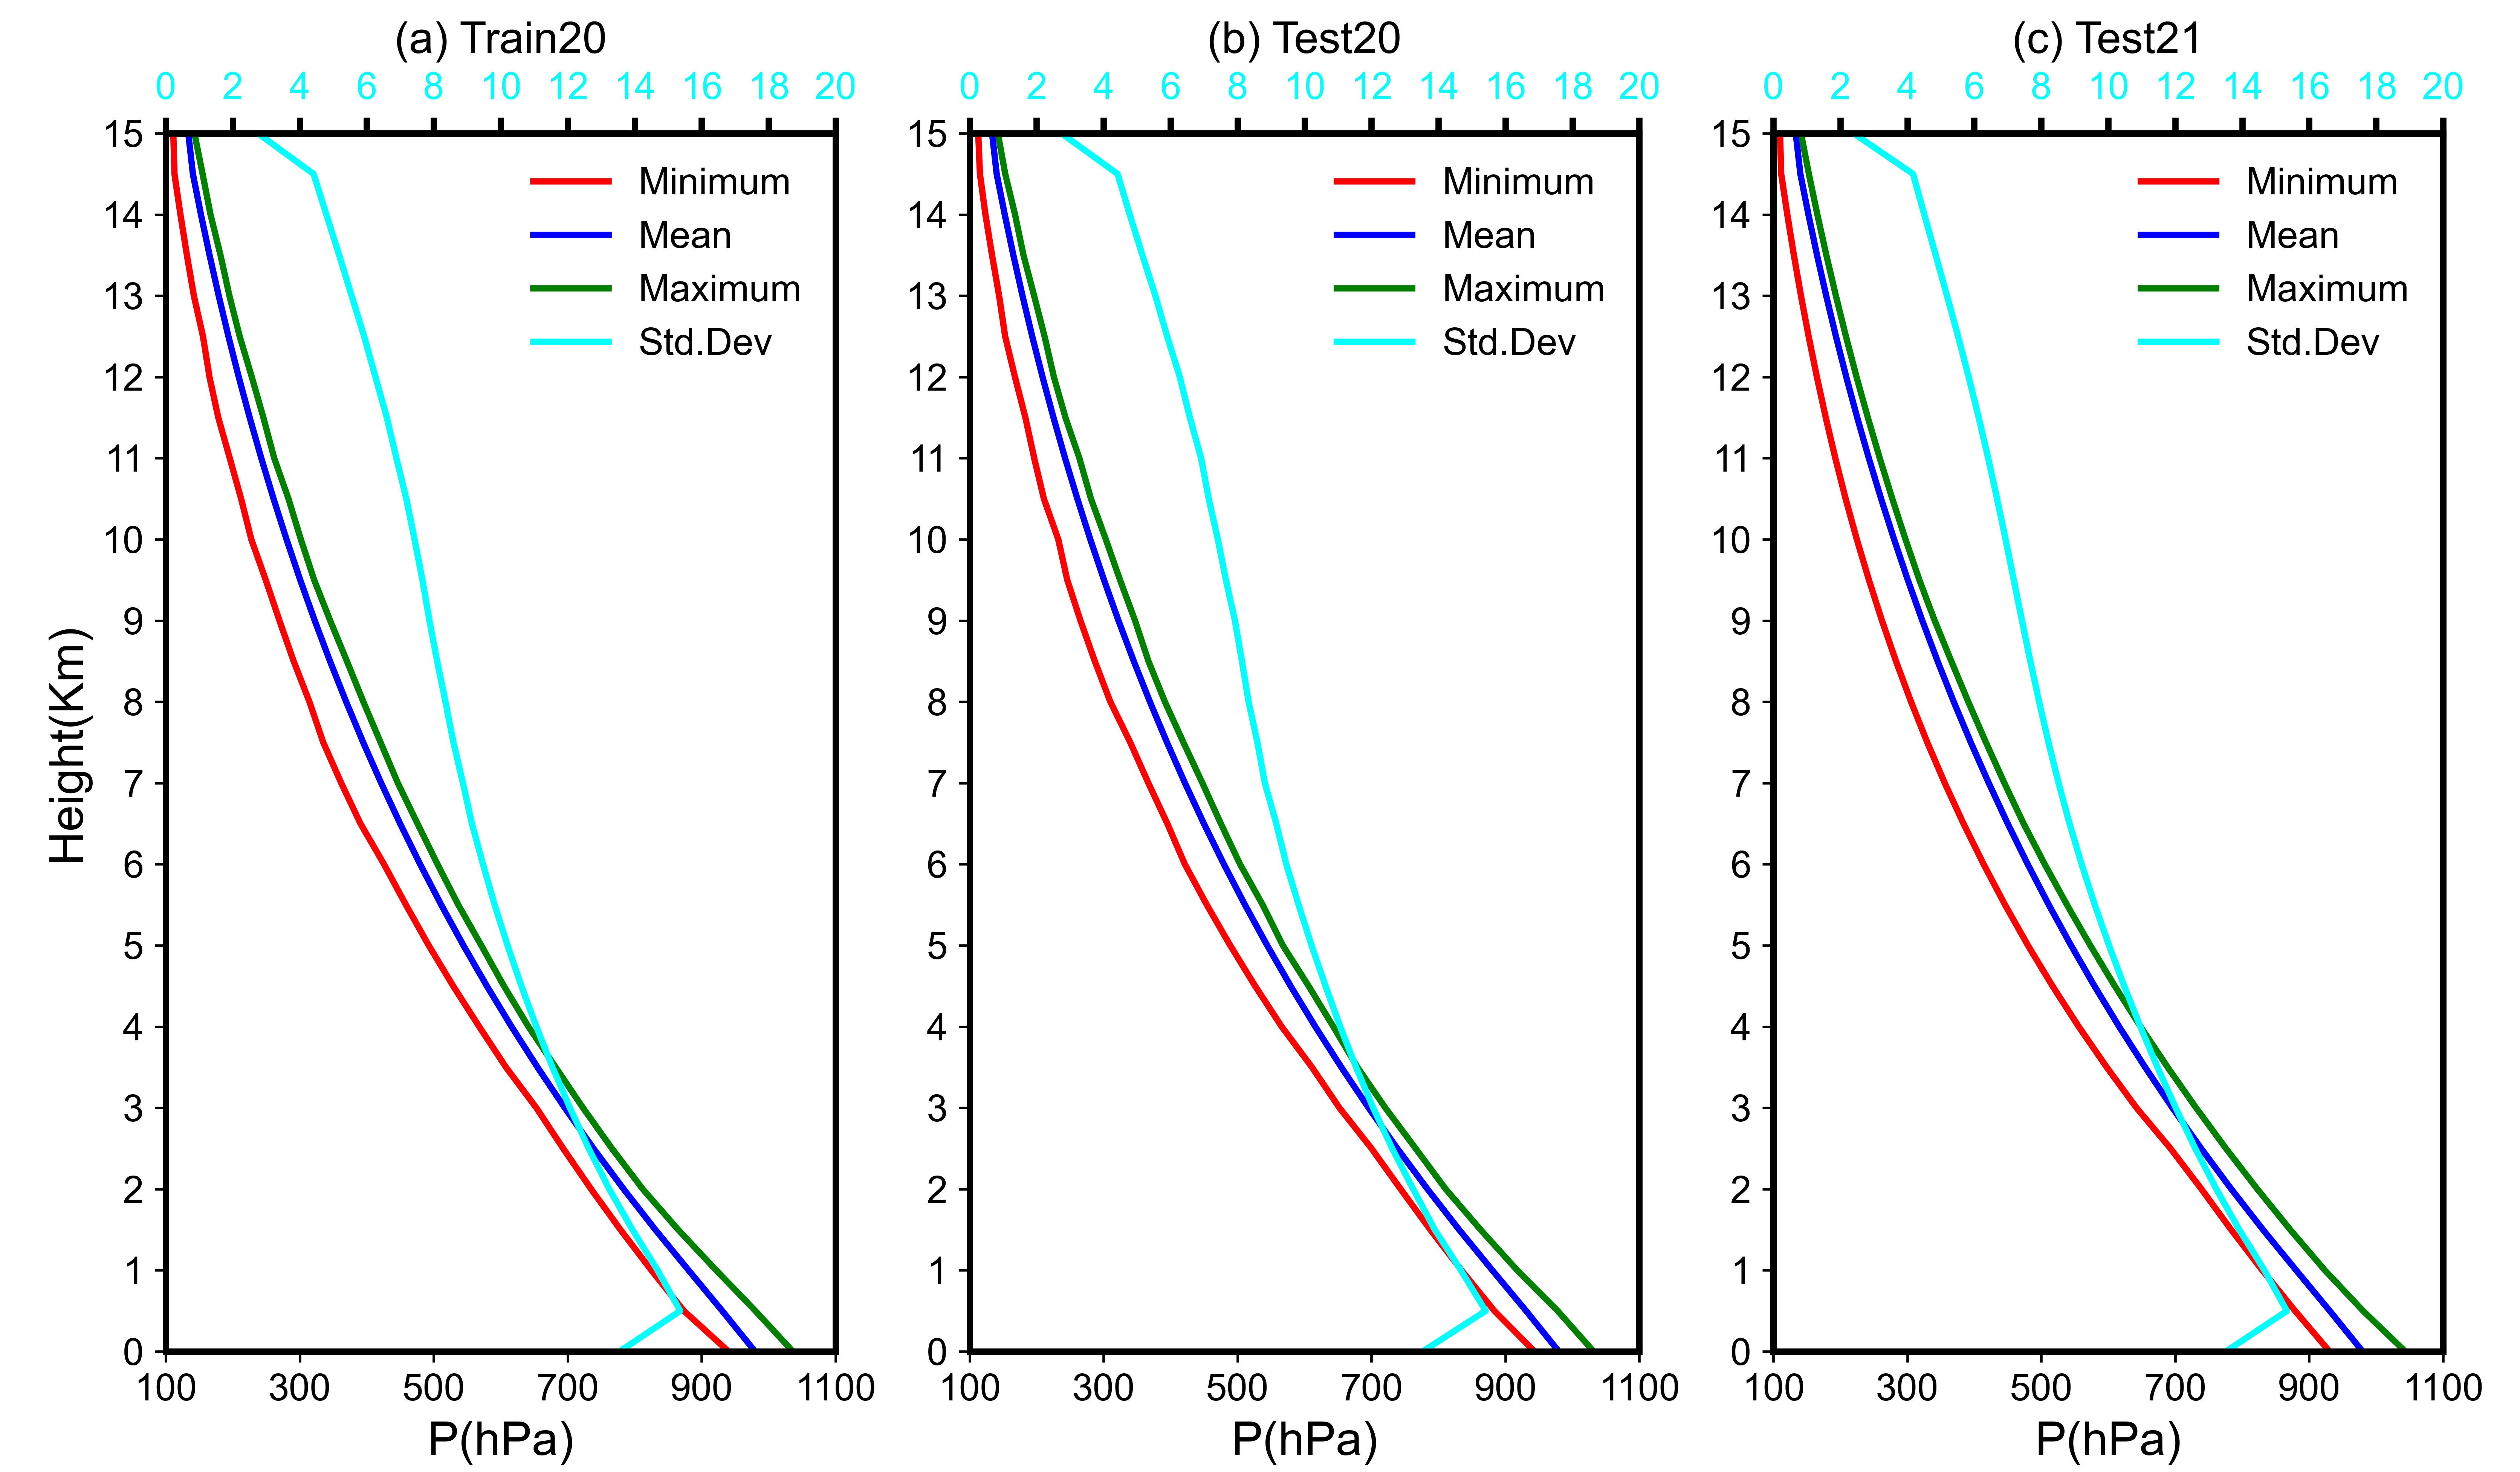
\includegraphics[width=14cm, height=8cm]{/Users/soumilhooda/Desktop/COSMIC_REPORT/NEW-FIGURES/prs-min-mean-max-std-stats-profile.png}
	\caption{Statistical analysis of pressure data obtained from wetPf2. Leftmost panel indicates the training data from 2020, middle panel is the testing data from 2020, rightmost panel indicates the testing data from 2021. The top x axis is used to plot the standard deviation scale. The points accumulated over the entire domain are used to generate these statistics.}
	\label{fig:img4}
\end{figure}


\begin{figure}[H]
	\centering
		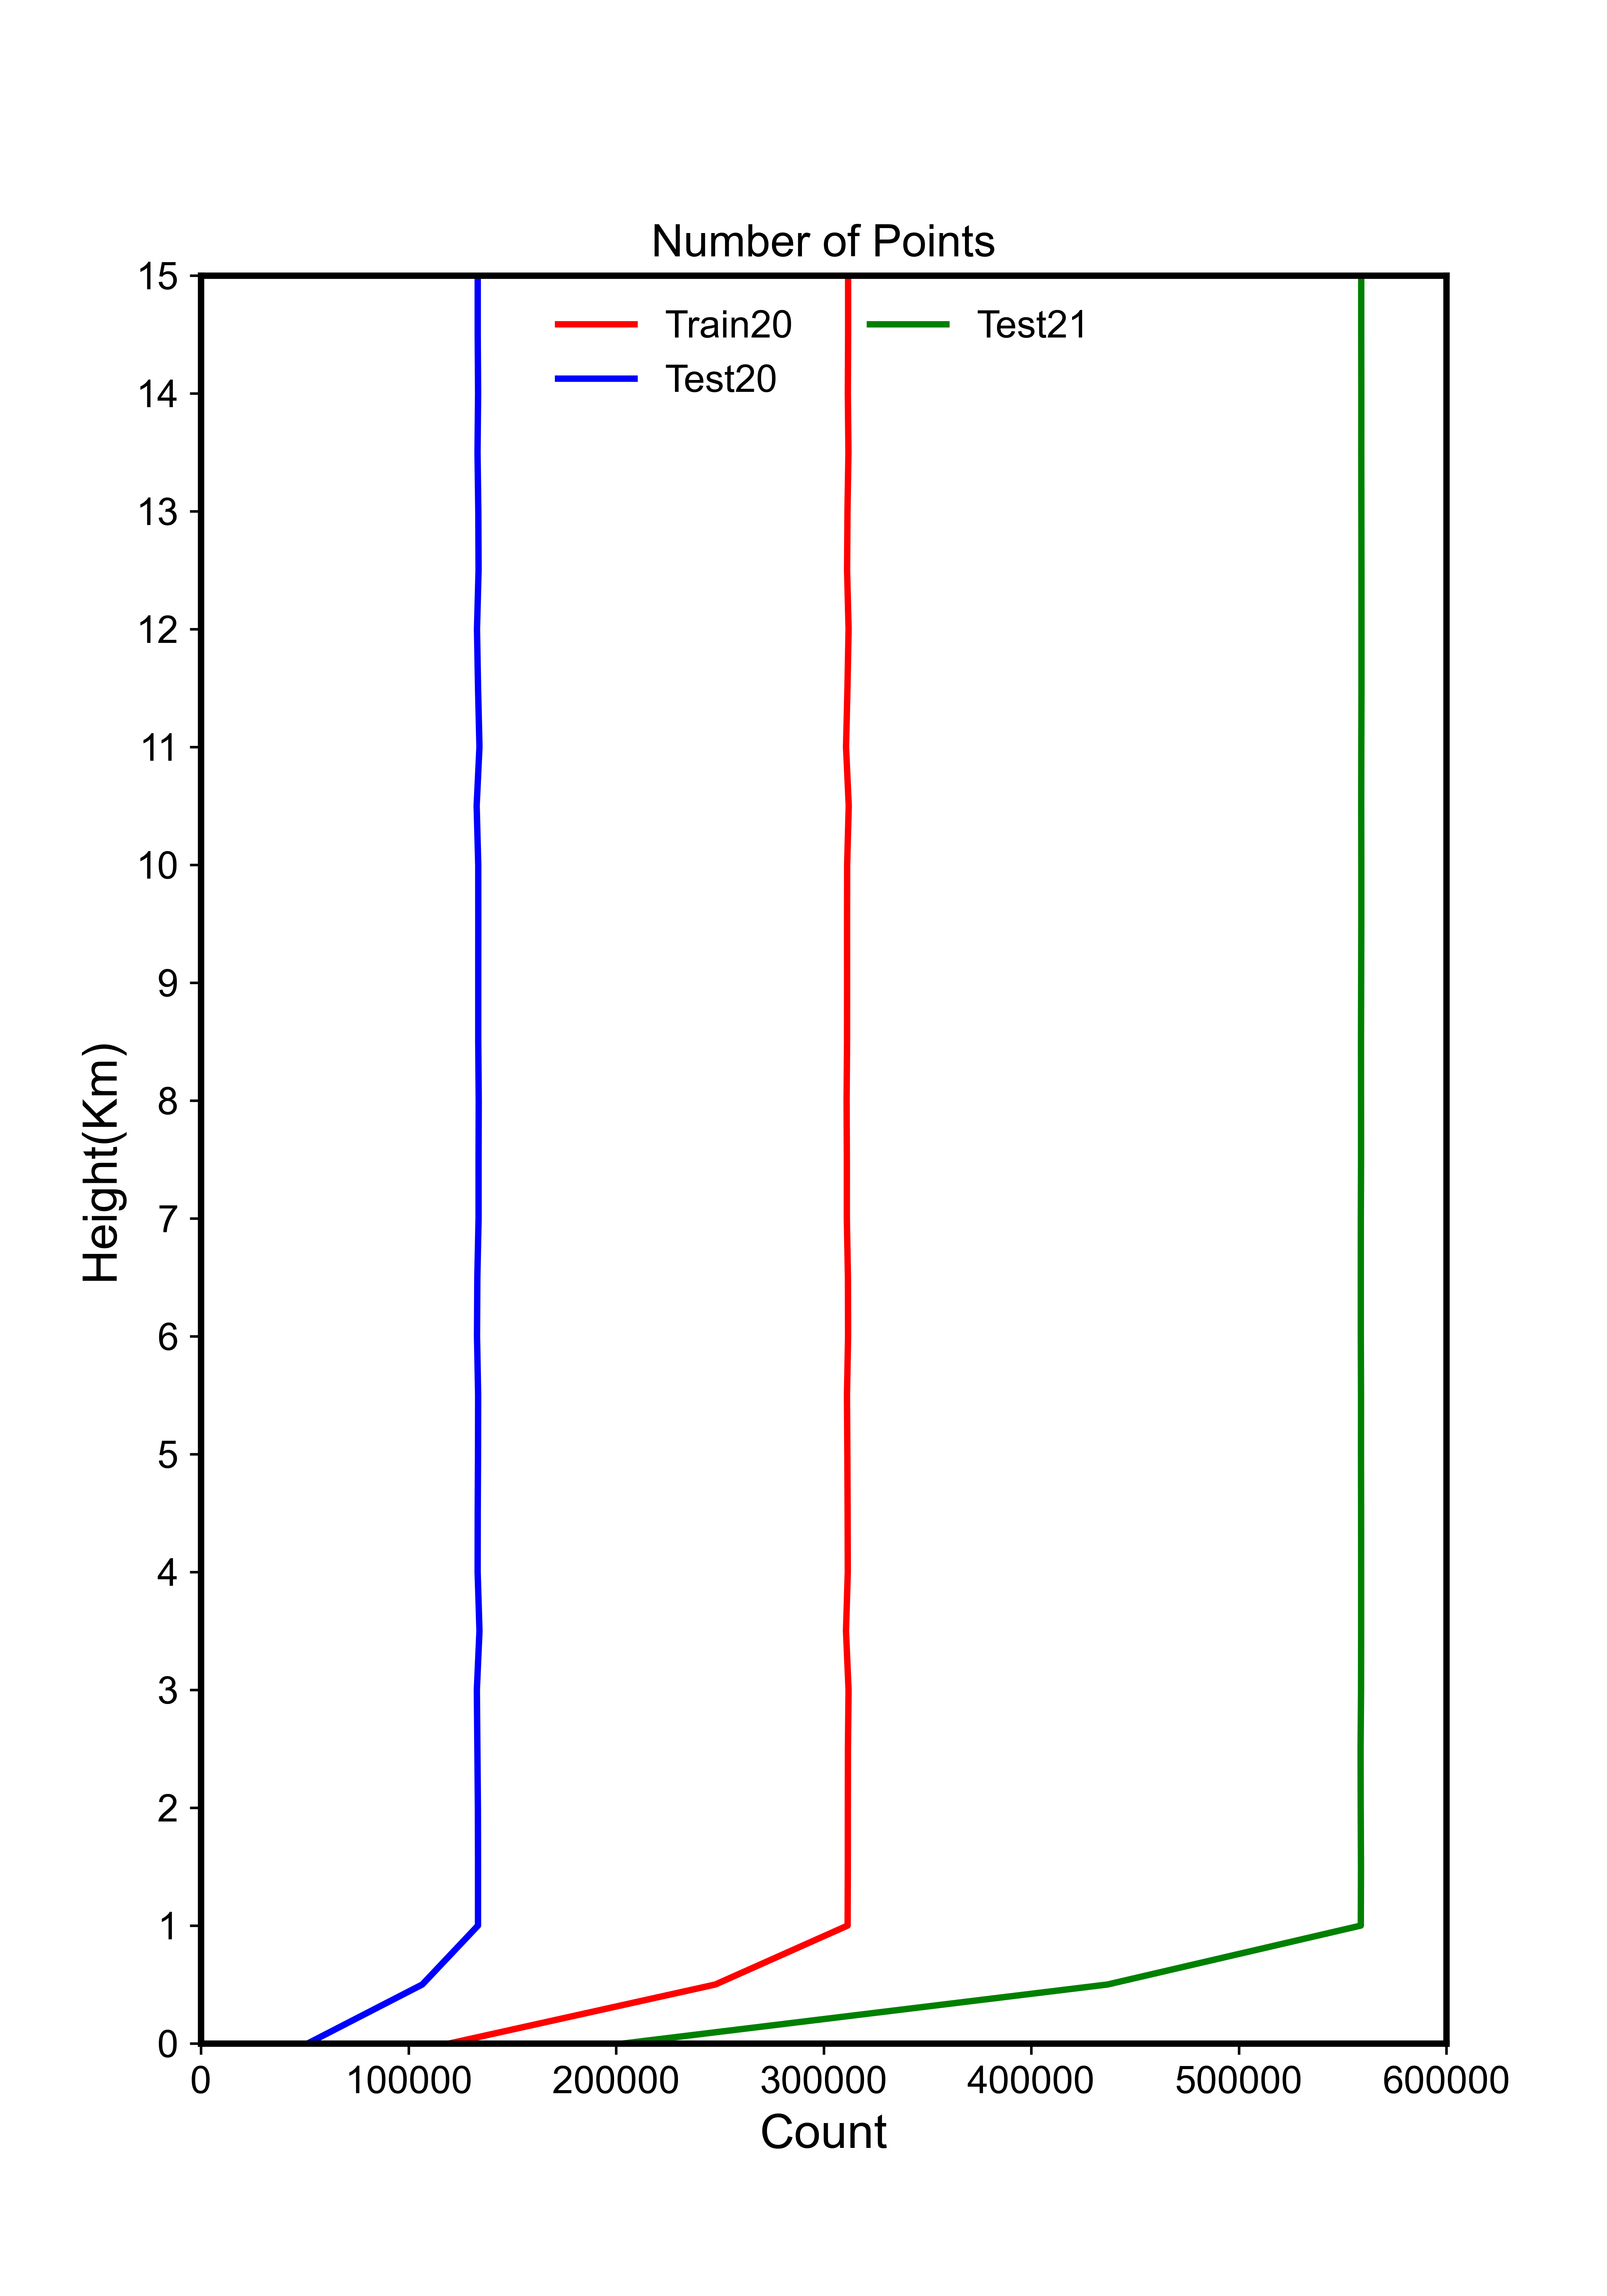
\includegraphics[width=0.7\linewidth, height=14cm]{/Users/soumilhooda/Desktop/COSMIC_REPORT/NEW-FIGURES/count-profile.png}
		\caption{Total number of points in various height ranges employed for model training and testing. The points have been accumulated over the entire domain.}
		\label{fig:img9}
\end{figure}
\begin{figure}[H]
		\centering
	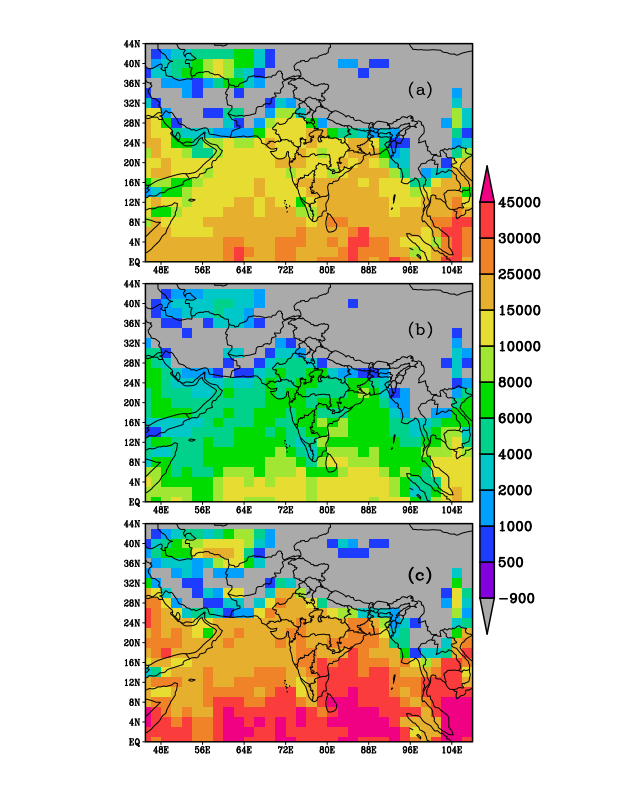
\includegraphics[width=12cm, height=20cm]{/Users/soumilhooda/Desktop/COSMIC_REPORT/images/dist-prs-count-train20-test20-test21.png}
	\caption{Spatial distribution of total number of points used for (a) training 2020 and (b) testing 2020 and (c) testing 2021 the model. The points have been accumulated over the entire height. The study's exclusion criteria eliminated areas with a color that is "gray", which are regions with surface elevation of more than 1000 m.}
	\label{fig:img22}
\end{figure}

\begin{figure}[H]
		\centering
		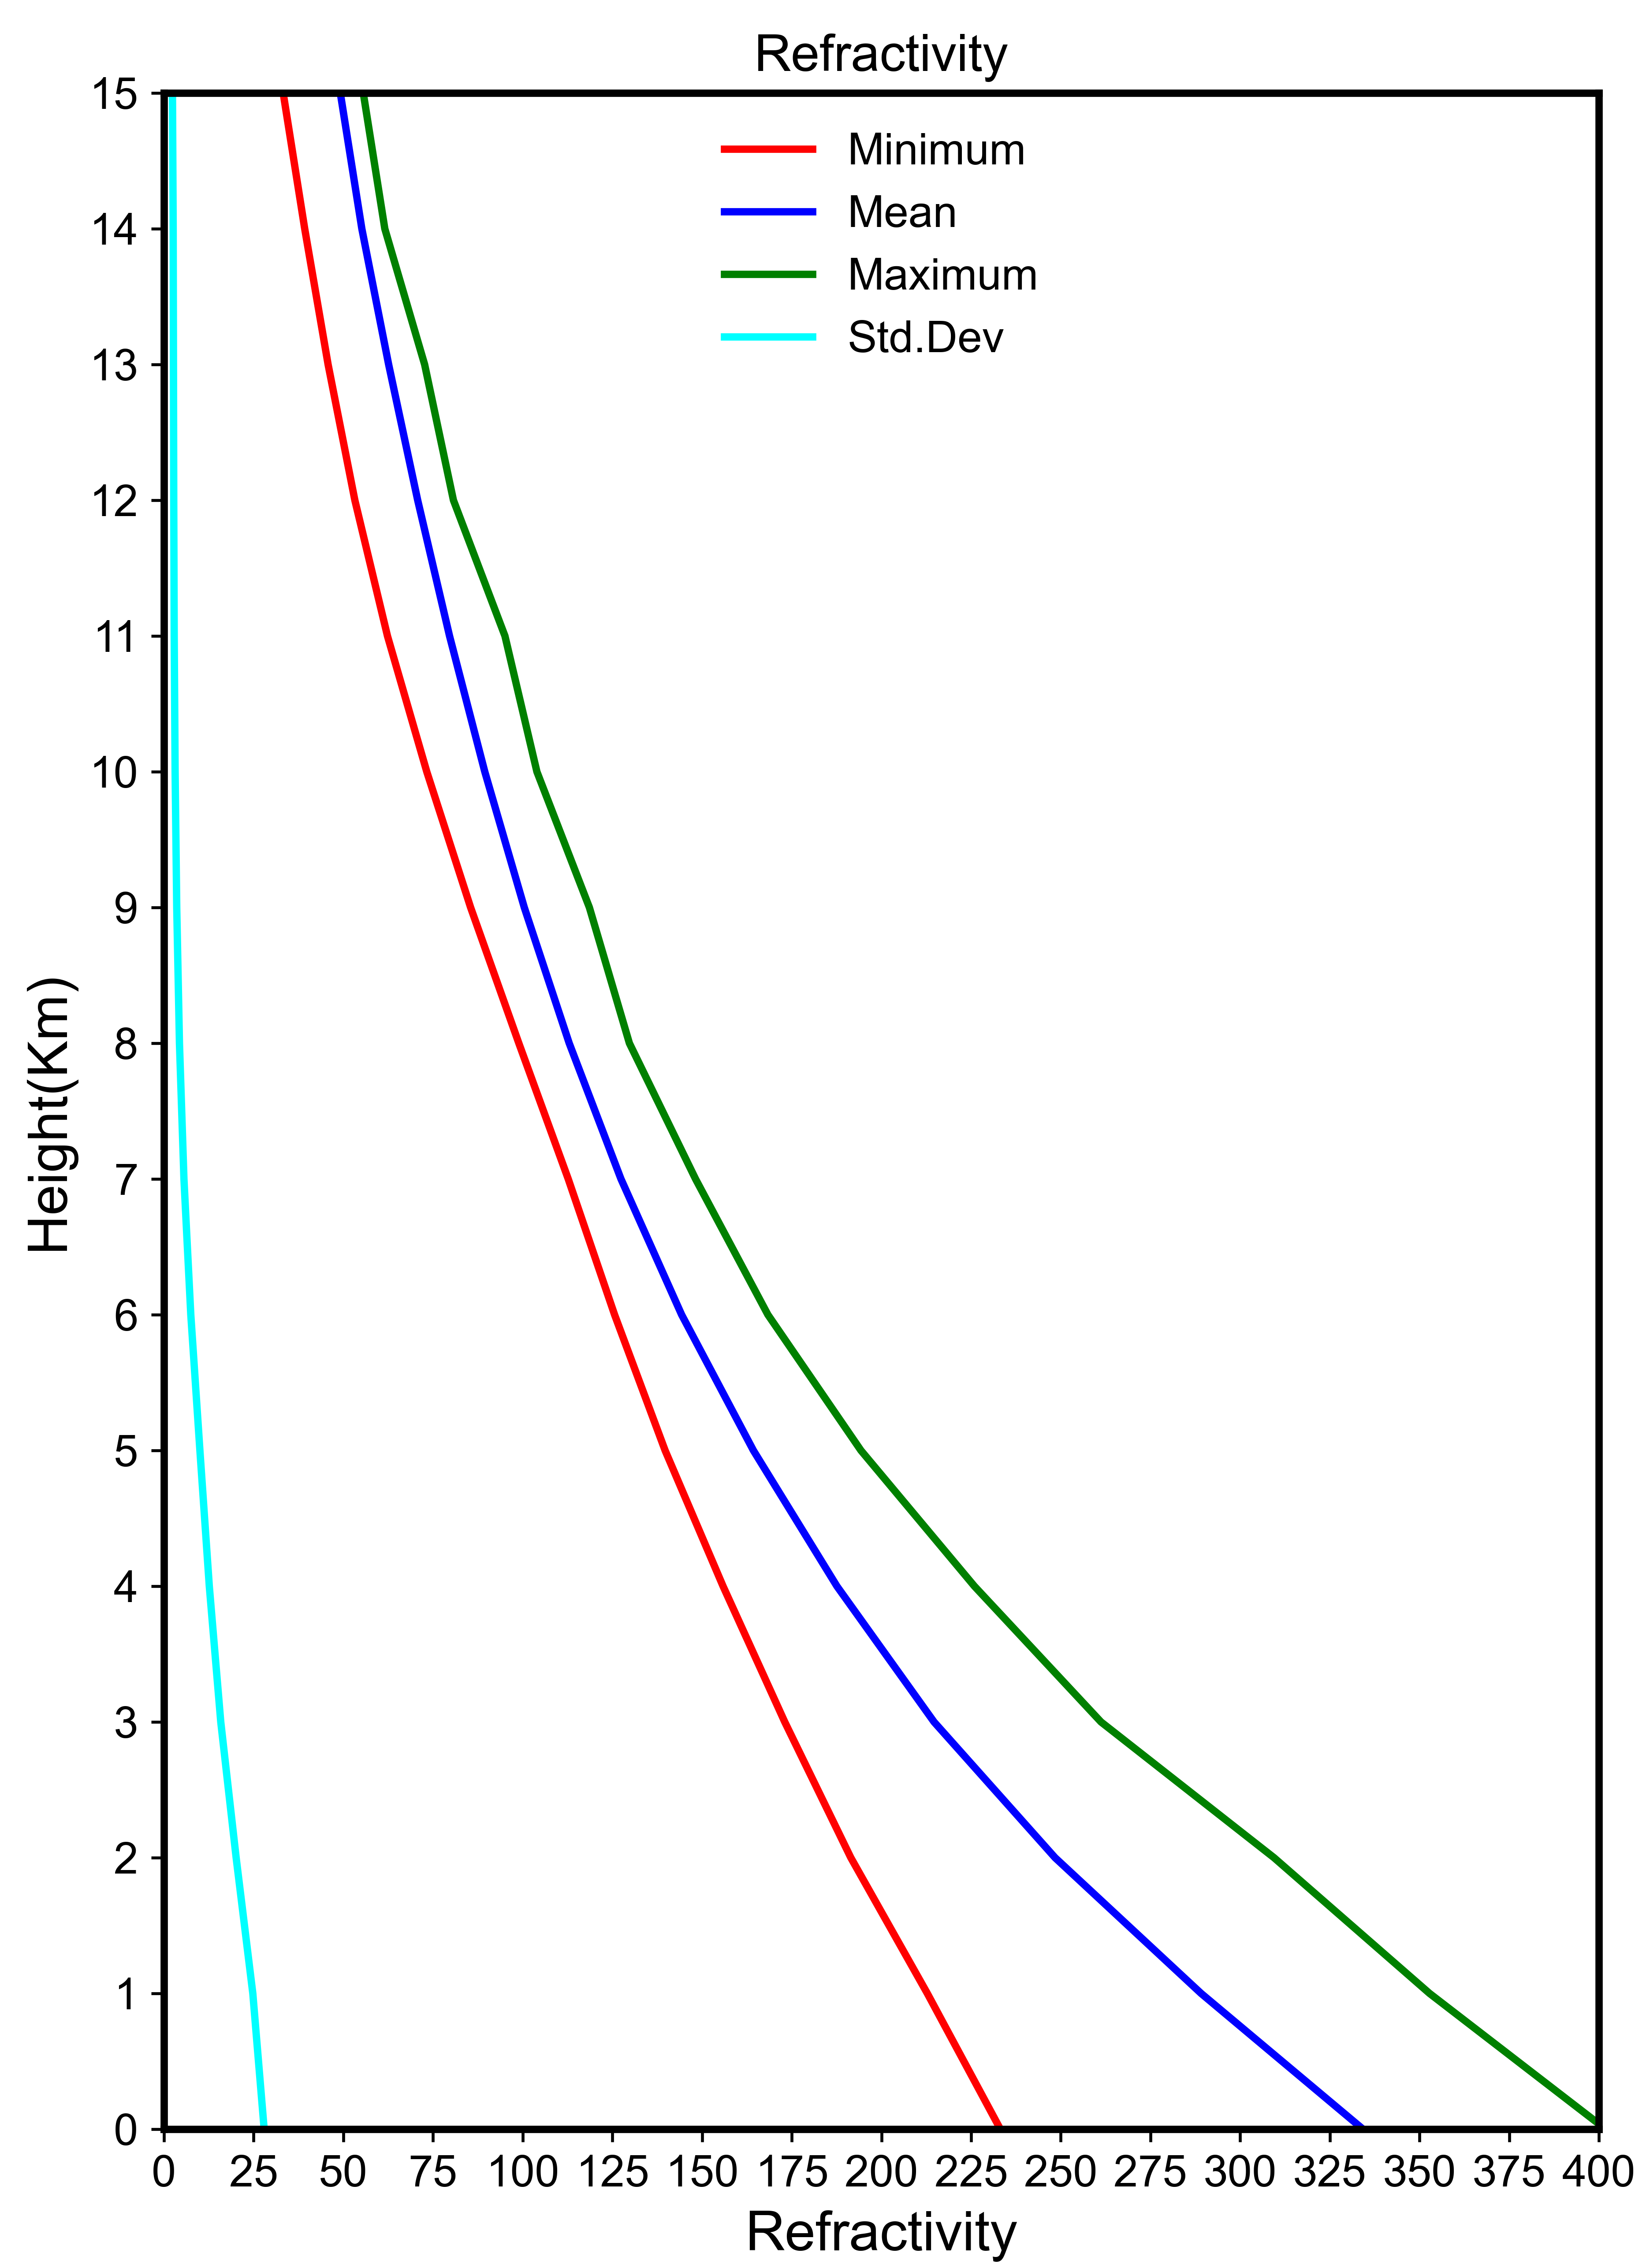
\includegraphics[width=8cm, height=10cm]{/Users/soumilhooda/Desktop/COSMIC_REPORT/NEW-FIGURES/refractivity-min-mean-max-std-profile.png}
		\caption{Statistics of the refractivity data derived using CDAAC thermodynamic profiles and the 3-term refractivity formulation. The data for years 2020 and 2021 over the selected domain are used to compile the statistics.}
		\label{fig:img8}
\end{figure}




\subsection{Methodology}

\noindent For our study we focussed only on the ANN owing to its simplicity and effective results as shown by \textit{Lasota} (2021). The ANN is an algorithm based on the works of \textit{Hassoun} (1995) that are highly used in its feed-forward multilayer perceptron (MLP) configuration. An input, one or more hidden layers, and an output are the three types of layers that make up a typical model. Multiple basic processing units known as neurons or nodes connect these layers. The number of nodes in these layers and the number of hidden layers are arbitrary and are determined by the complexity and volume of available data. Each neuron in a given layer of an MLP network is connected to every neuron in the layer above it, and the strength of each connection is expressed by a numerical weight that is determined during training. The backpropagation algorithm is typically used in iterative learning processes. The neural network receives input data repeatedly, multiplies it by connection weights, adds it all up, and then sends the result to the following layer. Finally, based on the discrepancies between predicted and actual outputs, the model's error is estimated in the final layer. The calculated error is then fed back into the model and used to modify the connections weight, reducing the model's error and bringing the outputs closer to the desired results.\\

\noindent In the upper troposphere, where water vapour pressure values are close to zero, our investigation during training found that the water vapour pressure values occasionally fit toward the negative. Therefore, we employed a sigmoid activation function to manage this circumstance. Water vapour pressure was normalised at input and re-normalised at the output with the maximum water vapour pressure value (34.6566 hPa) found in the training set, the same values were used to re-normalised for any independent datasets. To be able to use the sigmoid output activation function for water vapour pressure and linear output function for temperature-pressure, we build two different models that differ only in output activation as can be seen in Figure \ref{fig:img6} and Figure \ref{fig:img7}. 

\begin{figure}[H]
	\centering
	\begin{minipage}{0.45\textwidth}
		\centering
		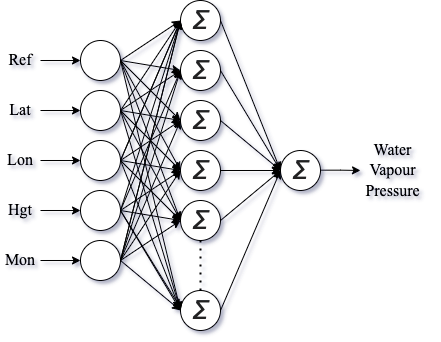
\includegraphics[width=\textwidth, height=6cm]{/Users/soumilhooda/Desktop/COSMIC_REPORT/images/model_evp.png}
		\caption{Model for retrieving water vapour pressure. Refractivity (Ref), height (Hgt), latitude (Lat), longitude (Lon) and month (Mon) are the input parameters, respectively. Note, that the inputs and outputs are for all 151 vertical levels (0 km to 15 km at a resolution of 100 m).}
		\label{fig:img6}
	\end{minipage}
	\hfill
	\begin{minipage}{0.45\textwidth}
		\centering
		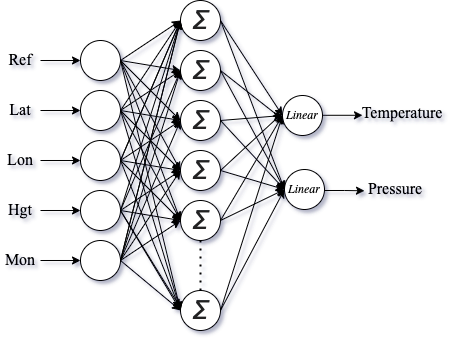
\includegraphics[width=\textwidth, height=6cm]{/Users/soumilhooda/Desktop/COSMIC_REPORT/images/model_tmpprs.png}
		\caption{Model for retrieving pressure and temperature. Refractivity (Ref), height (Hgt), latitude (Lat), longitude (Lon) and month (Mon) are the input parameters, respectively. Note, that the inputs and outputs are for all 151 vertical levels (0 km to 15 km at a resolution of 100 m).}
		\label{fig:img7}
	\end{minipage}
\end{figure}

\noindent  Differing to model parameters, which must be set beforehand before training, hyperparameters are configuration parameters that govern the learning process.
Hyperparameters have a significant impact on how well a model performs, and choosing the best set of variables to include in a model is one of the most difficult tasks involved. Owing to parameters developed by \textit{Lasota} (2021) we zero down and grid search around the following parameters,
\begin{itemize}
	\item Hidden layers : 1, 2 and 3
	\item Hidden layer neurons: 50, 125, 250 and 500
	\item Dropout: 0 and 0.1
	\item Activation functions: rectified linear unit, leaky rectified linear unit, sigmoid and linear
	\item Epochs: 10, 50, 100, 500 and 1000
	\item Batch: 100, 500, 1000, 2000 and 10000
\end{itemize}

\noindent We use holdout validation as we want to emphasise on the independence of the testing data from across both years 2020 and 2021. The Adam optimisation algorithm first developed by \textit{Kingma and Ba} (2014) was used to determine weights. We end up with optimal parameters at 1 hidden layer with 500 neurons, no dropout with sigmoid activation for the hidden layer at 500 batch size for 500 epoch, for both our models. \\


\section{Results and Discussion}

\noindent  The scatter plot between the actual and retrieved water vapour pressure is shown in Figure \ref{fig:scatt-evp-train20-test20-test21} for the training and testing samples from 2020 and totally independent testing data from 2021. The root mean square error (RMSE) for the training (Train20), testing (Test20), and independent data set of the year 2021 (Test21) are in the range 0.196 hPa, 0.196 hPa and 0.24 hPa. The bias between the retrieved and actual water vapor pressure is very negligible. The retrieval error for the 2020 training and testing data sets is roughly 5.5\%, whereas the error for the 2021 entirely independent testing data set is about 7\%. As a result, the developed model displays excellent accuracy and negligible bias. In order to evaluate how retrieval errors vary vertically, Figure \ref{fig:img19} shows the bias (such as mean differences), root mean square error, and standard deviation of differences between actual and retrieved water vapour pressure for training and testing data sets. For training and testing data for the year 2020, the lower troposphere exhibits a positive (i.e., model underestimate) bias of the order of 0.1 hPa. The RMSE is approximately 0.5 hPa close to the surface, and it decreases as height increases. As previously seen from the statistics of the data sets, the water vapour pressure decreases with height and, hence, error likewise decreases with height. Furthermore, because bias is low, the RMSE and standard deviation appear to be identical. When compared to the training and testing data from 2020, the model's retrieved water vapour pressure for the testing data from 2021 has a little bit greater bias, RMSE and standard deviations. The model overestimates the water vapour pressure by 0.2 hPa to 0.3 hPa (negative mean differences). But only by 0.1 hPa are the RMSE and standard deviation greater in 2021 than in 2020. Therefore, even with a completely independent data set, the overall model performs excellently. \\

\noindent For the training-testing split (2020) and independent (2021) datasets, Figure \ref{fig:img11} displays the spatial distribution of the bias, RMSE, and standard deviation of the differences between actual and retrieved water vapour pressure. In the domain, bias ranges from 0 hPa to 0.02 hPa for the 2020 test and from -0.1 hPa to 0.2 hPa for the 2021 test. For the 2020 test and the 2021 test, respectively, the RMSE varies across the domain from 0.05 hPa to 0.45 hPa and from 0.12 hPa to 0.60 hPa. For the tests in 2020 and 2021, the standard deviation ranges from 0 hPa to 0.02 hPa and from -0.1 hPa to 0.2 hPa, respectively, across the domain. Furthermore, it is noteworthy to observe that RMSE and standard deviation increase as we move from lower to higher latitudes, with the equatorial region having the lowest errors. Our additional investigation (not provided) shows that the association between refractivity and water vapour pressure decreases as we move from the tropics, where the water vapour pressure is higher, to the higher latitudes, where the water vapour pressure is lower. As a result of the decreased association between refractivity and water vapour pressure, larger errors are anticipated in the water vapour pressure retrievals over higher latitudes. \\

\noindent Overall, the vertically averaged errors in retrieving water vapour pressure are 0.196 hPa, 0.196 hPa, and 0.240 hPa for training (Train20), testing (Test20), and independent testing (Test21), respectively. The water vapour pressure retrieved errors in this study are significantly less than the error reported by \textit{Lasota} (2021), which was 0.41 hPa. This could be for two reasons: first, this study only presents the retrieval accuracy for the Indian region, whereas \textit{Lasota} (2021) reported accuracy for the global region (mainly global oceanic regions). Second, unlike \textit{Lasota} (2021), who developed the model using COSMIC-2 refractivity and ERA5 thermodynamic profiles, we developed the model based on the simulated refractivity utilising wetPf2 data. \\


\begin{figure}[H]
	\centering
	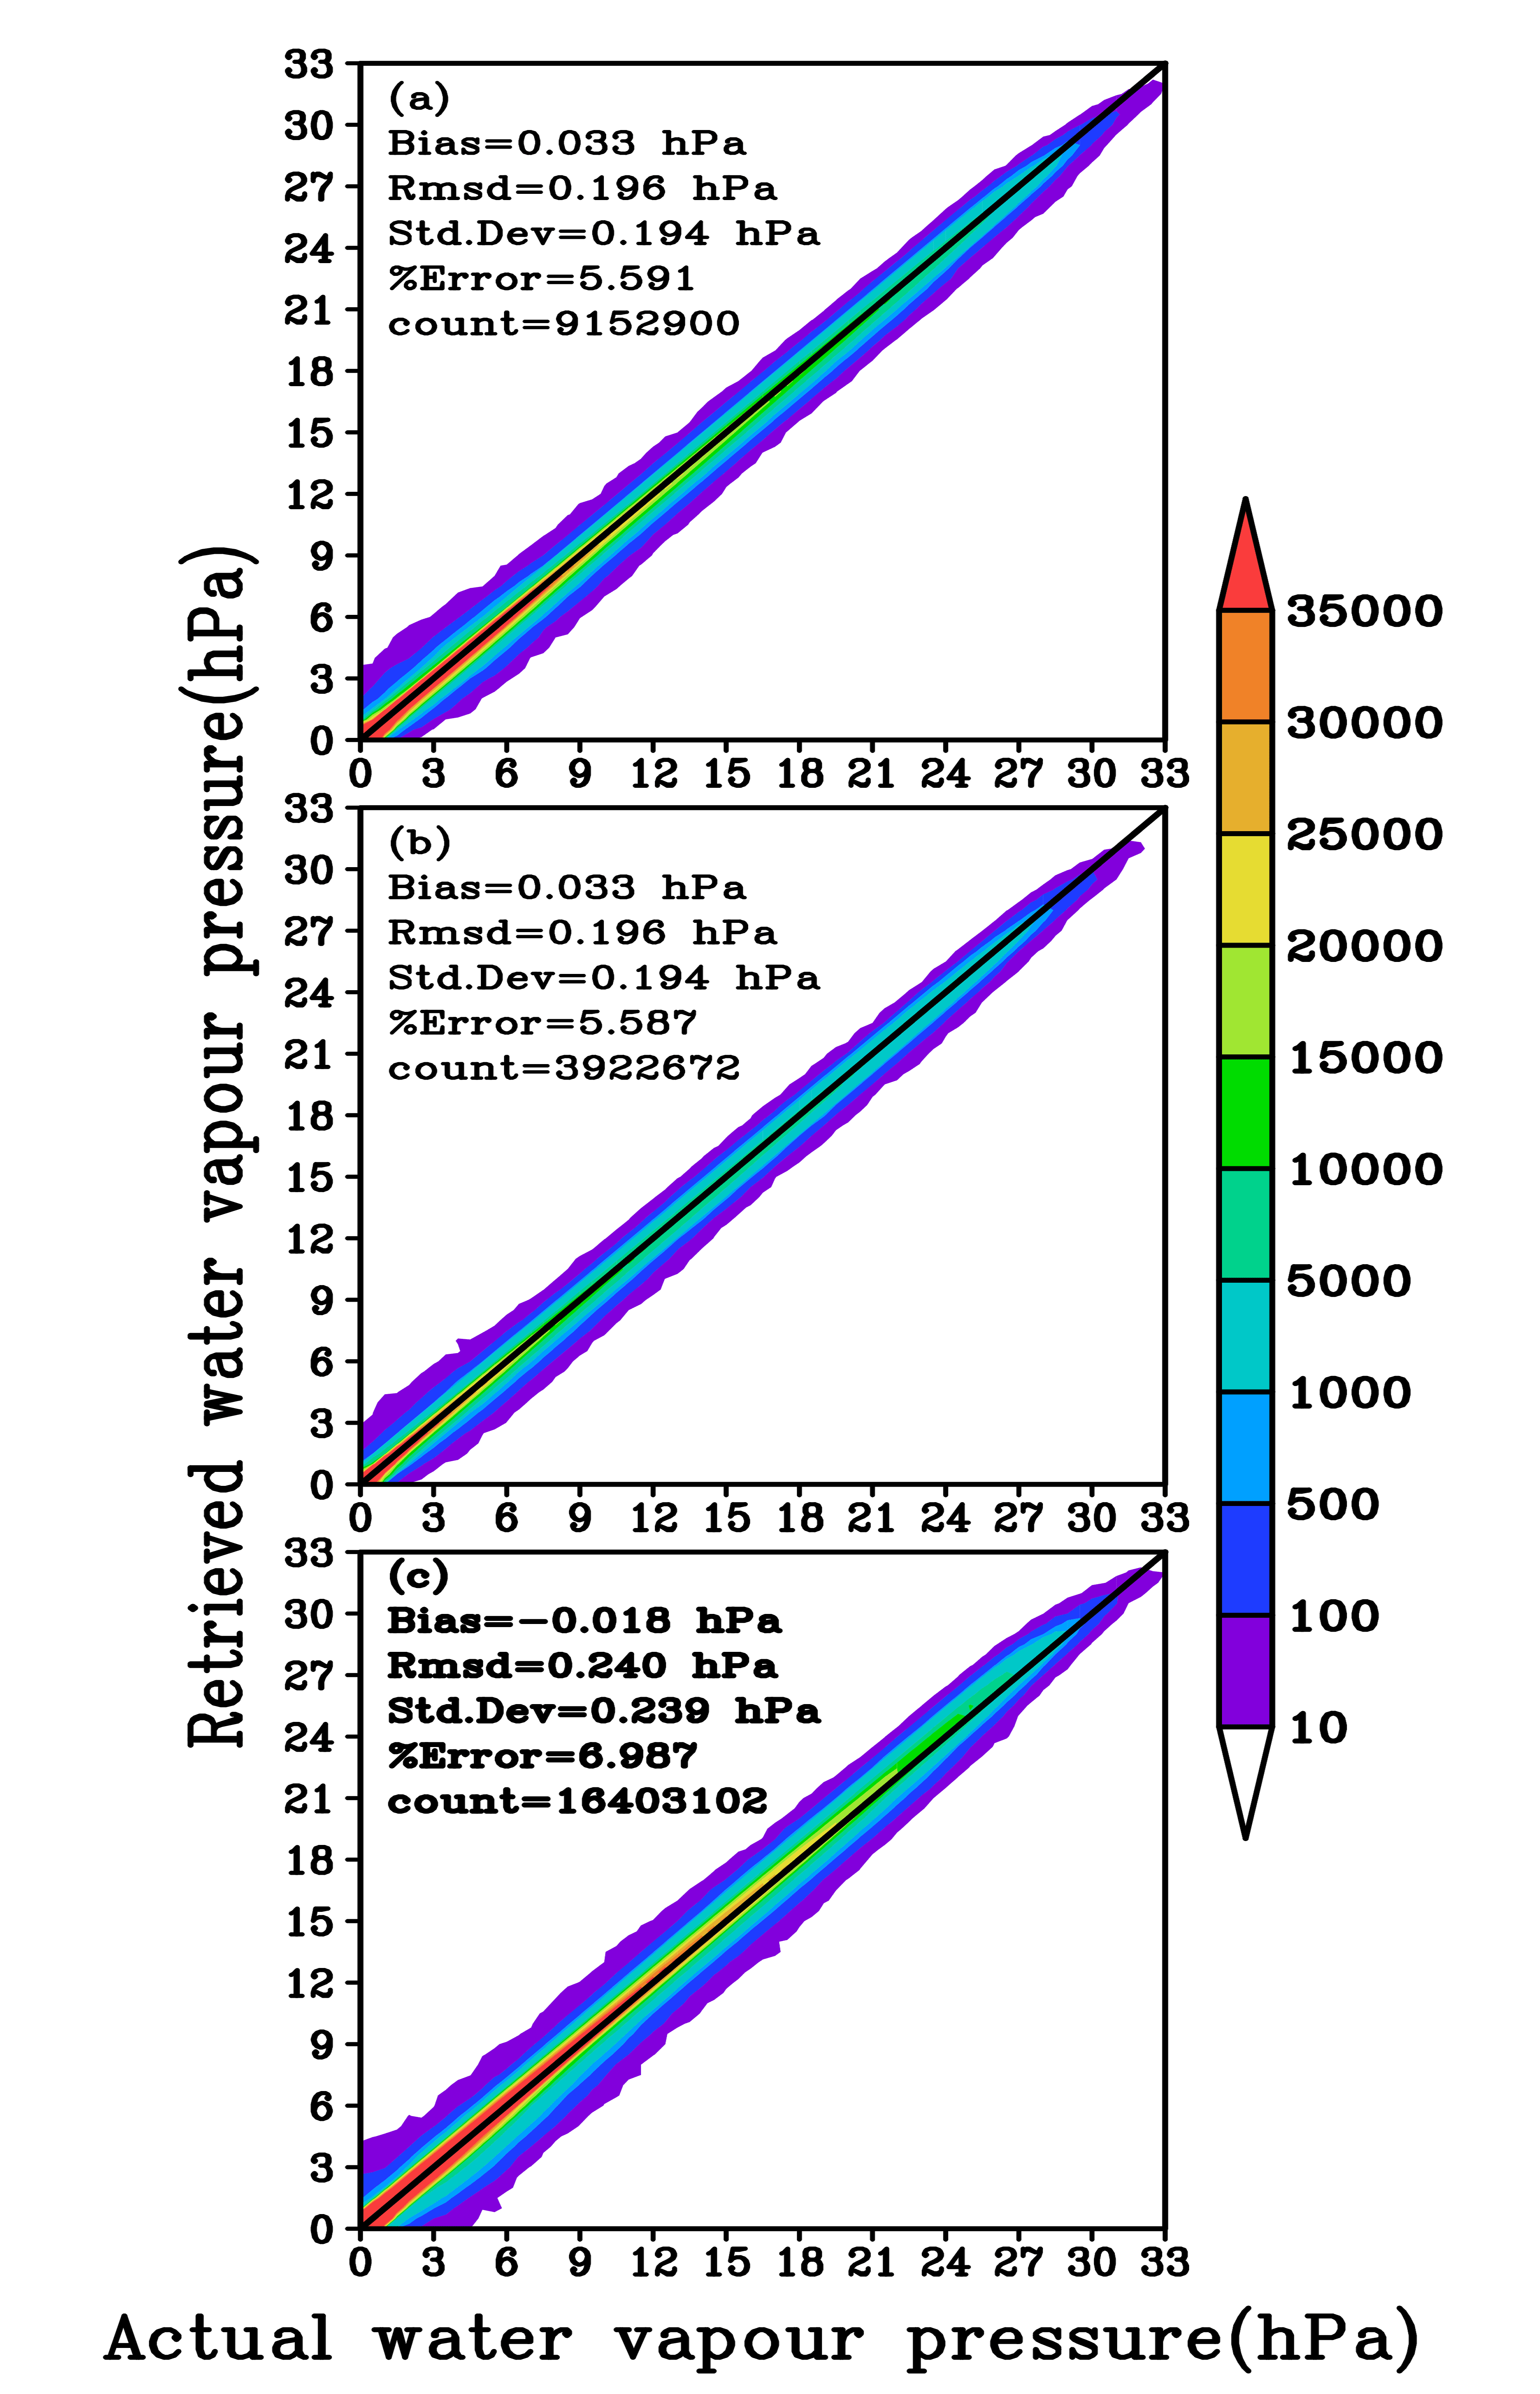
\includegraphics[width=0.7\textwidth, height=12cm]{/Users/soumilhooda/Desktop/COSMIC_REPORT/NEW-FIGURES/scatt-evp-train20-test20-test21.png}
	\caption{Scatter plot of actual versus retrieved water vapour pressure (a) for the training data set in 2020, (b) for testing data set in 2020, and (c) for completely independent data set fot the year 2021. Color bar represents the number of observations available for each water vapour pressure bin. This figure is based on data that has been accumulated over all vertical levels and the whole domain.}
	\label{fig:scatt-evp-train20-test20-test21}
\end{figure}
\begin{figure}[H]
\centering
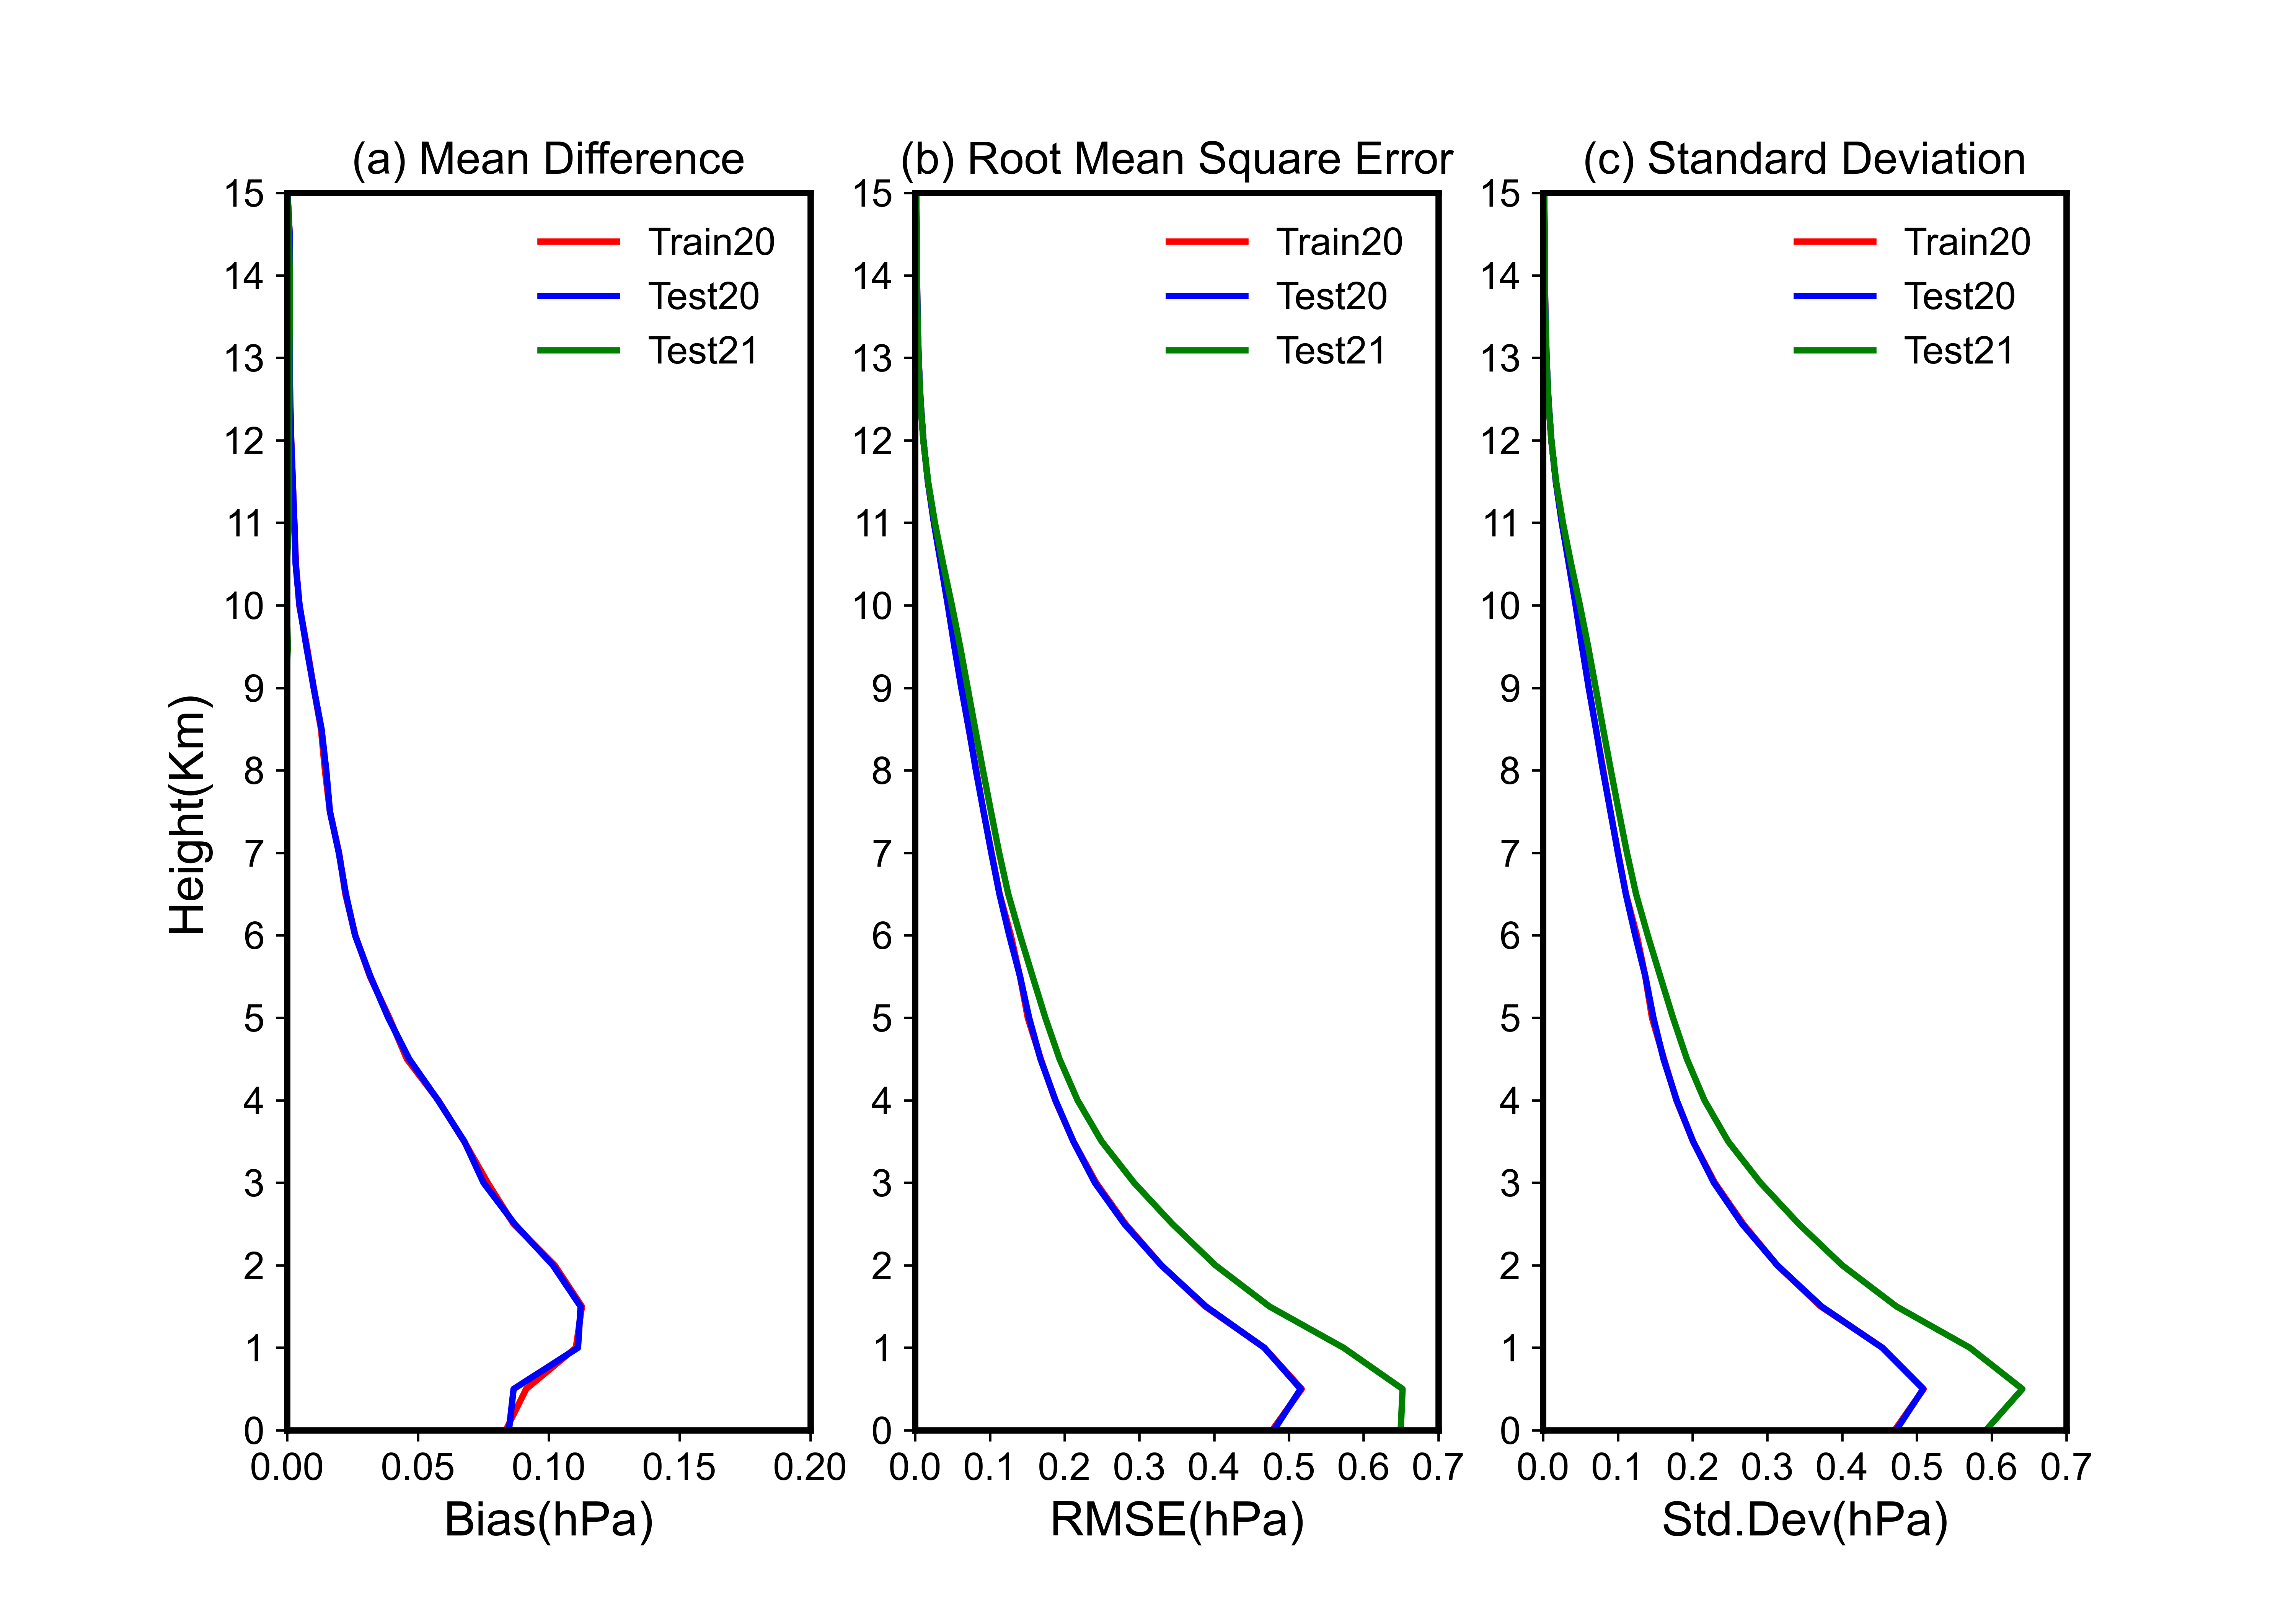
\includegraphics[width=\textwidth, height=7cm]{/Users/soumilhooda/Desktop/COSMIC_REPORT/NEW-FIGURES/evp-bias-rmsd-std-profile.png}
\caption{Vertical profiles (a) bias (i.e. mean differences), (b) root mean square error (RMSE), and (c) standard deviation (Std.Dev) of the difference between actual and model retrieved water vapour pressure, for training and testing data sets. The data acquired over the entire domain was used to create the figure. }
\label{fig:img19}
\end{figure}
\begin{figure}[H]
	\centering
	\begin{subfigure}{0.32\textwidth}
		\centering
		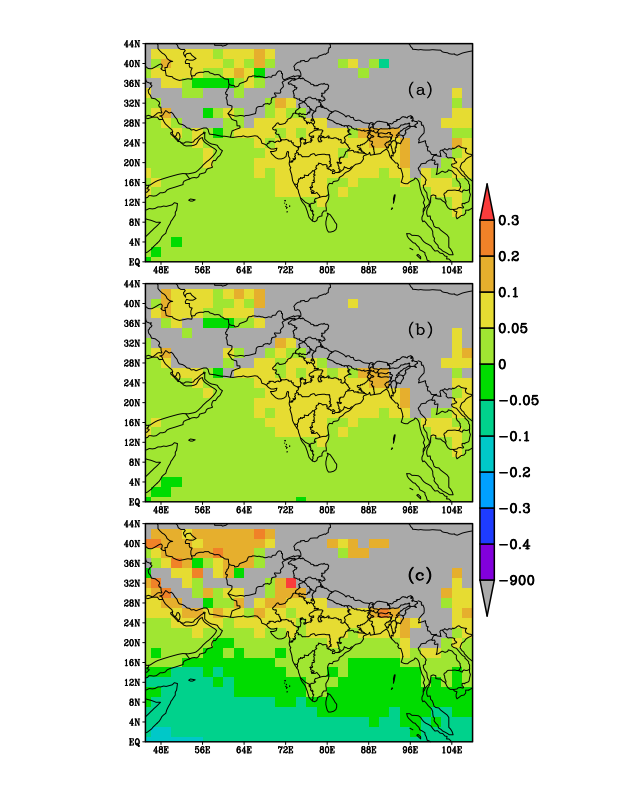
\includegraphics[width=\textwidth, height=9.5cm ]{/Users/soumilhooda/Desktop/COSMIC_REPORT/images/dist-evp-bias-train20-test20-test21.png}
	\end{subfigure}
	\hfill
	\begin{subfigure}{0.32\textwidth}
		\centering
		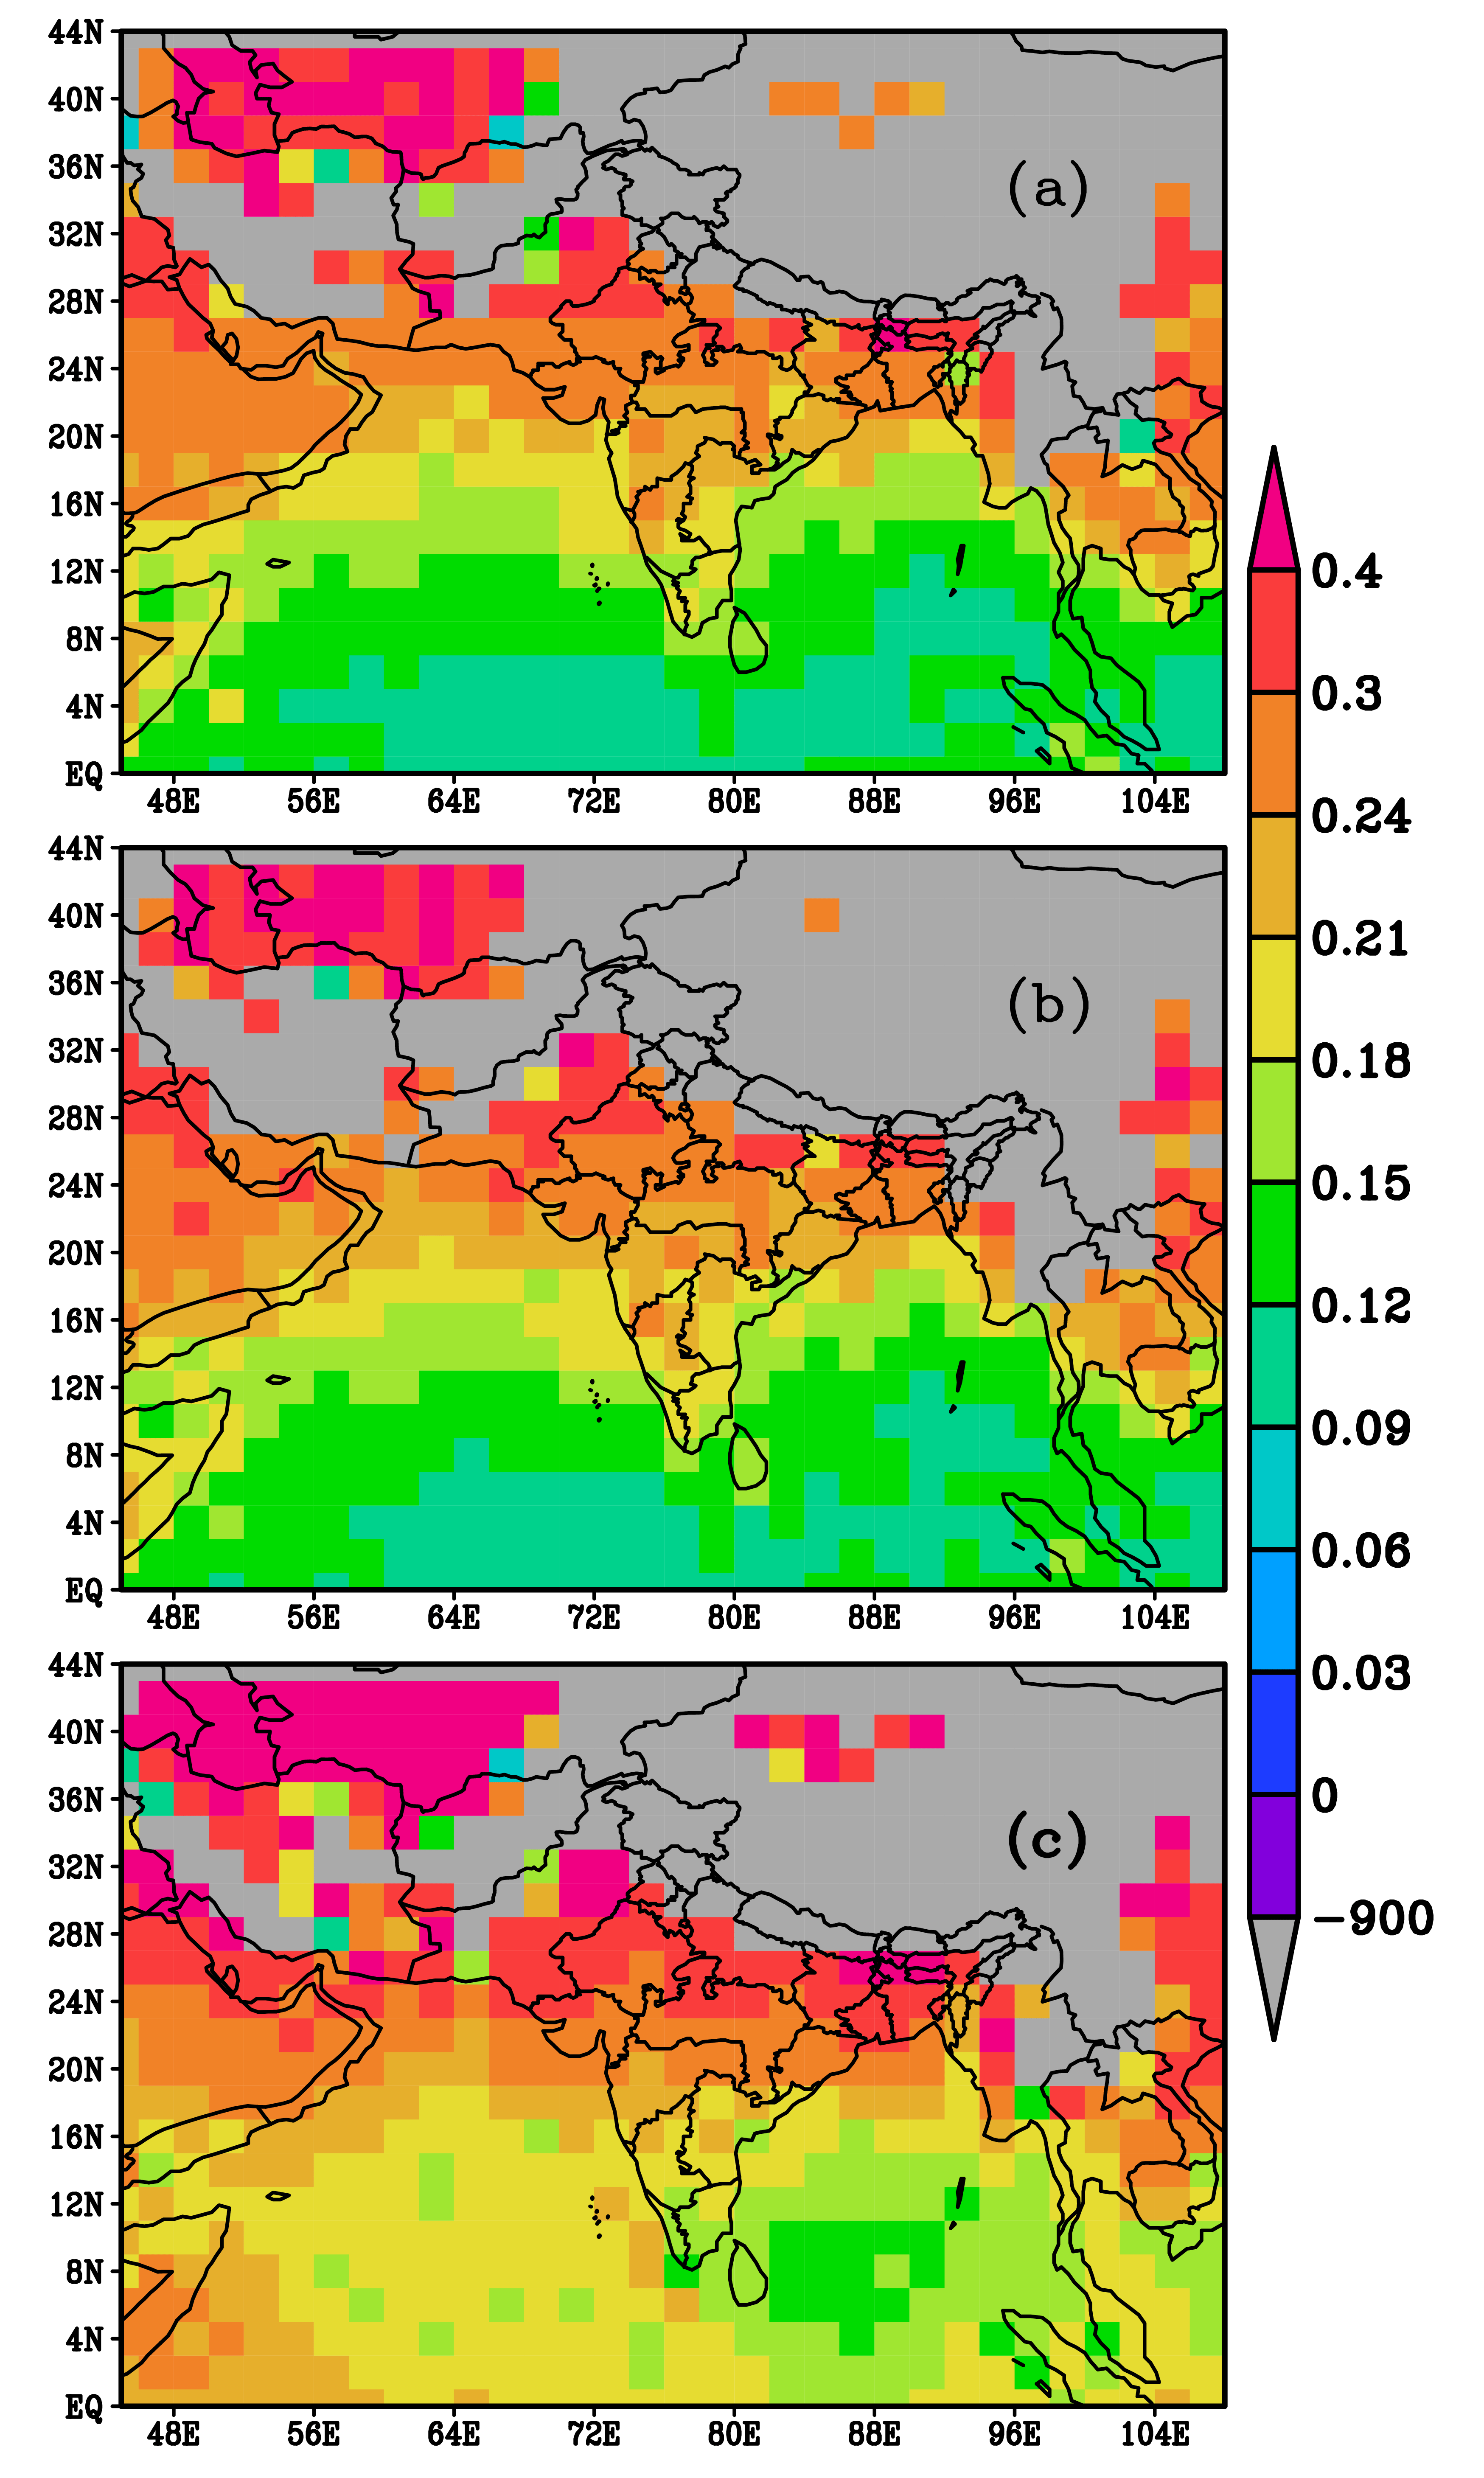
\includegraphics[width=\textwidth, height=9.5cm]{/Users/soumilhooda/Desktop/COSMIC_REPORT/images/dist-evp-rmsd-train20-test20-test21.png}
	\end{subfigure}
	\hfill
	\begin{subfigure}{0.32\textwidth}
		\centering
		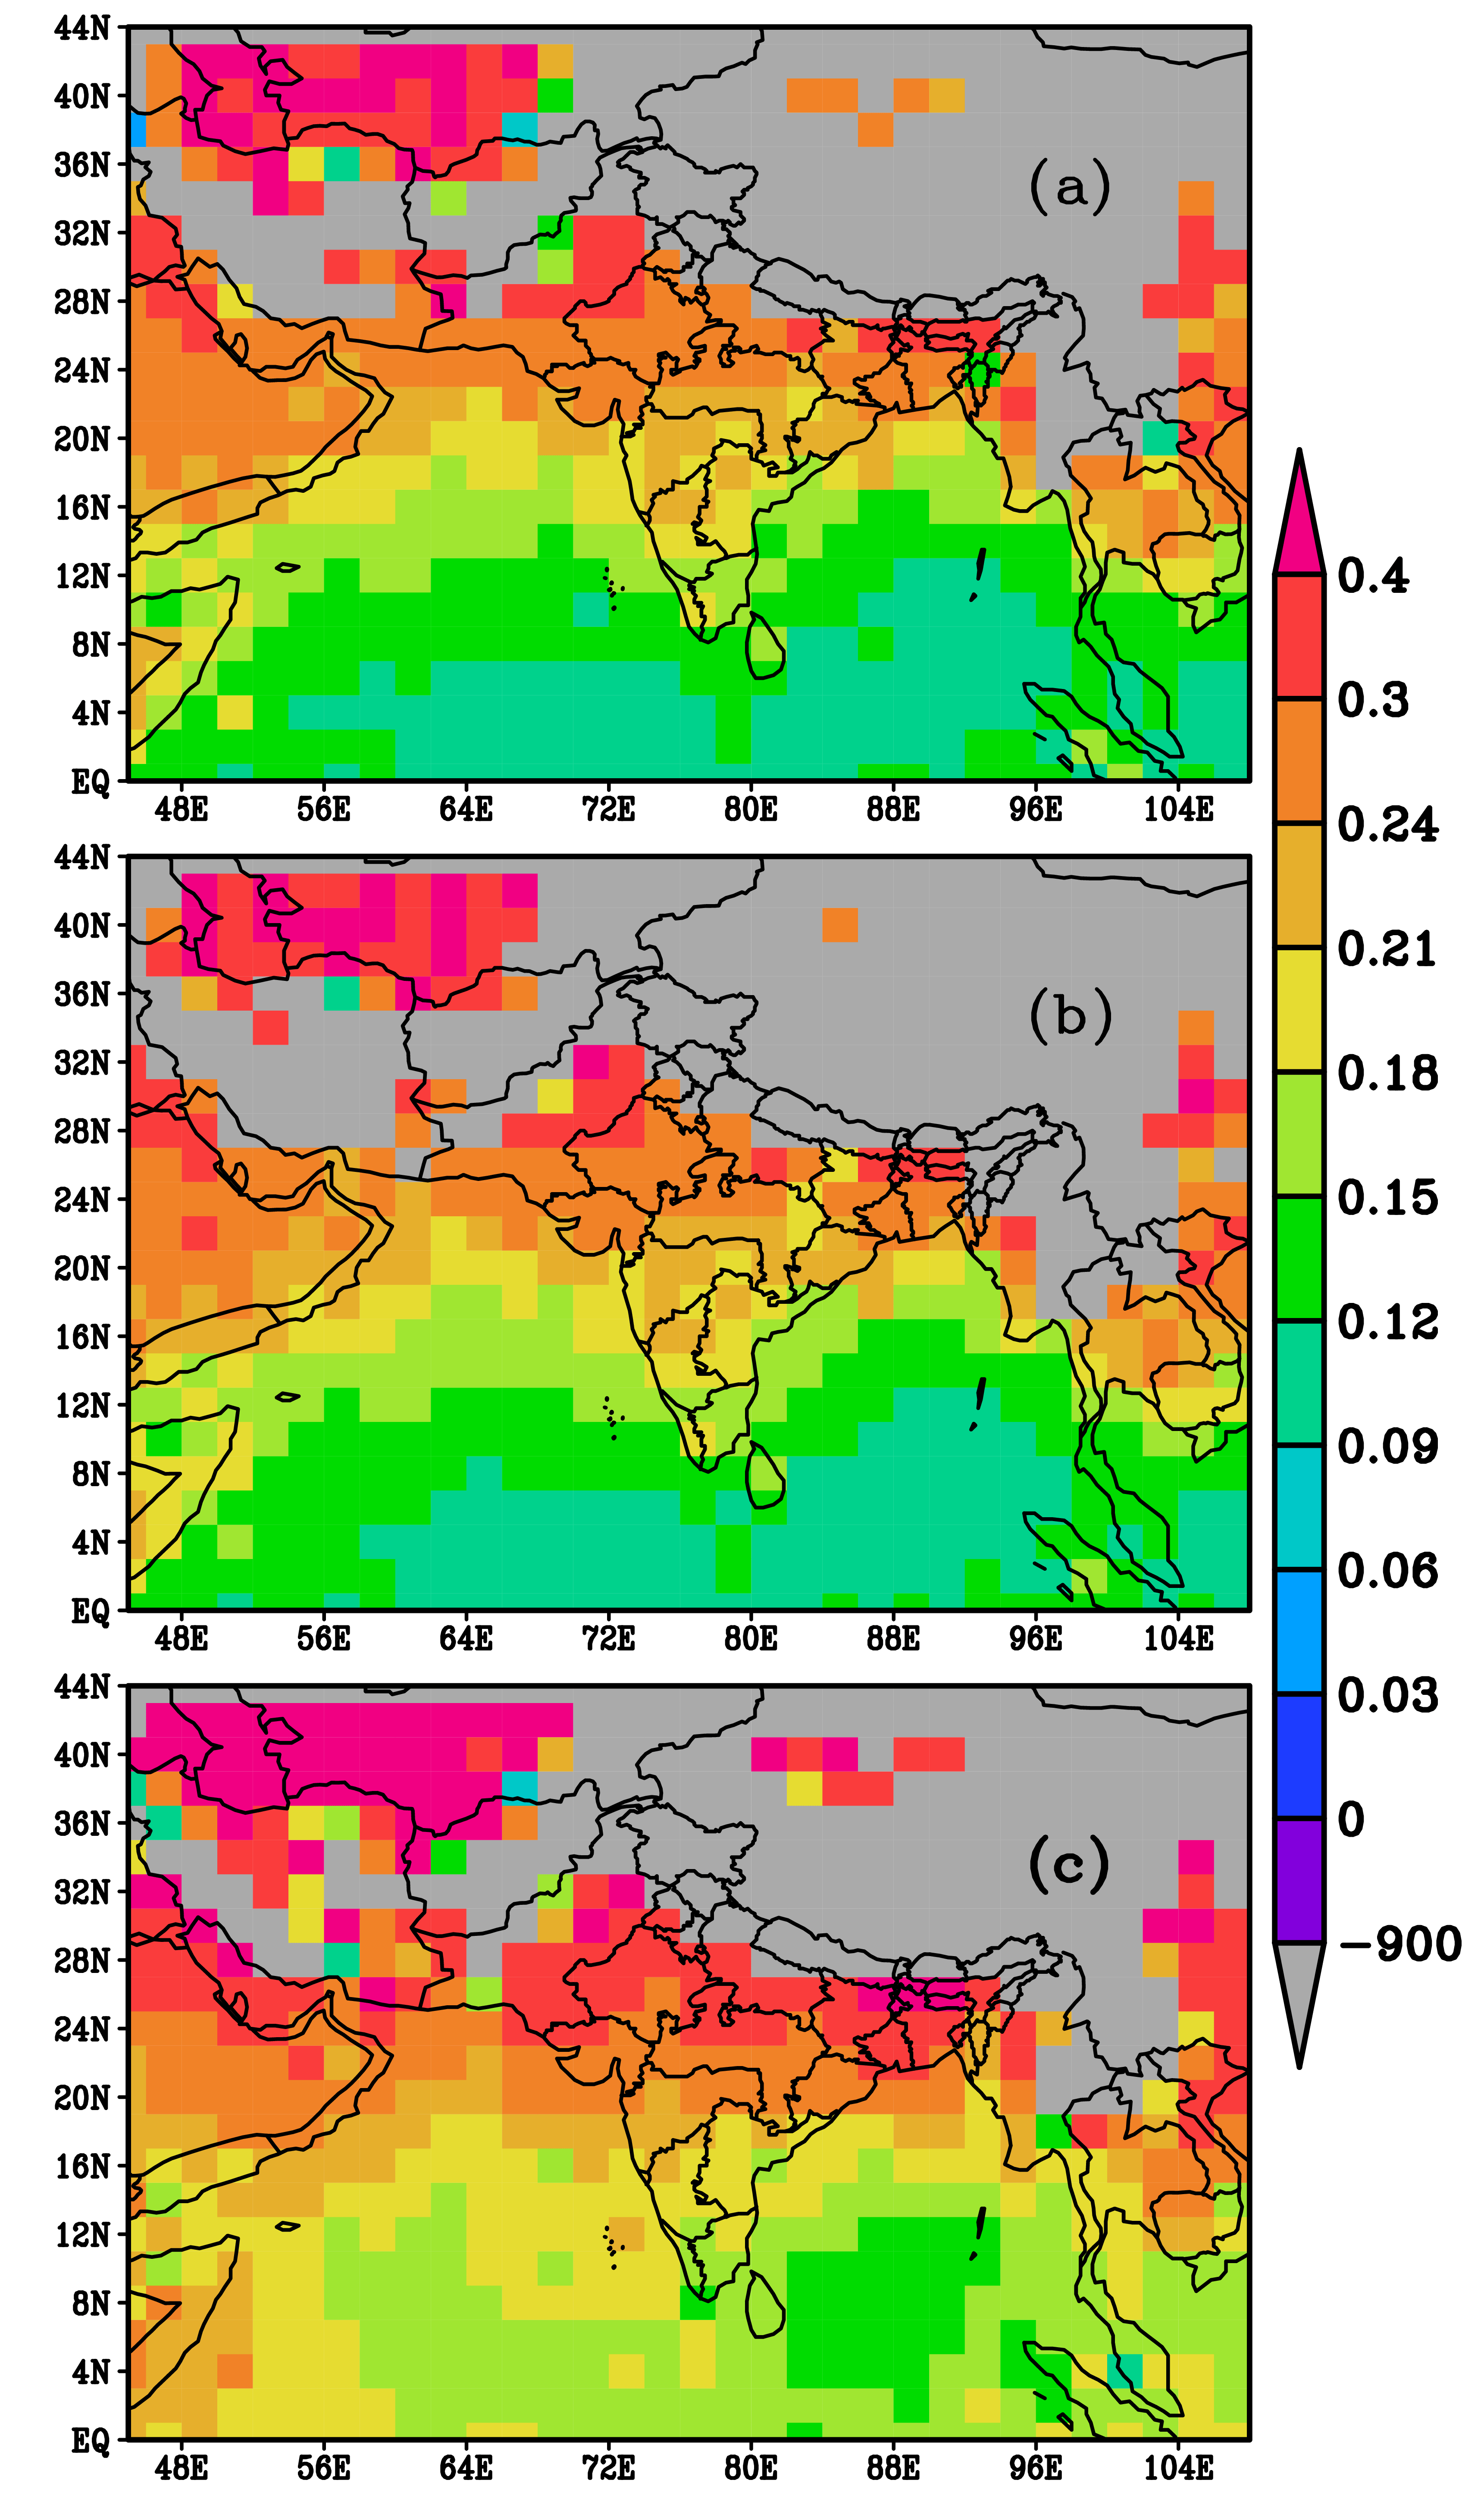
\includegraphics[width=\textwidth, height=9.5cm ]{/Users/soumilhooda/Desktop/COSMIC_REPORT/images/dist-evp-std-train20-test20-test21.png}
	\end{subfigure}
	\caption{Spatial pattern of mean diffferences (i.e. bias), root mean square error (RMSE) and standard deviation (Std.Dev) of the differences between actual and model retrieved water vapour pressure. First column is for bias, second is for RMSE, and third is for standard deviation. Panels (a), (b) and (c) in each column represent the training data set for 2020, testing data set for 2020 and the testing data for 2021. The figure is produced using data collected across all heights.}
\label{fig:img11}
\end{figure}

\noindent The scatter plot between actual and retrieved temperature for the training (Train20) and testing (Test20 and Test21) datasets are displayed in Figure \ref{fig:img20}. For Train20, Test20, and Test21, the RMSE between actual and retrieved temperature is $~1.3 K, ~1.3 K, and ~1.6 K$, respectively. The bias (mean difference) between the actual and retrieved temperatures is roughly -0.2 K, but the bias for Train20 and Test20 is negligible. Overall, retrieval errors for training and testing (Test20 and Test21) datasets are comparable. The temperature retrieval errors are comparable to those published by \textit{Lasota} (2021), who reported retrieval errors of the order of 1.4 K in training and around 1.7 K for the testing. The vertical profiles of the differences between actual and retrieved temperature for the training and testing datasets are shown in Figure \ref{fig:img21} for bias, RMSE, and standard deviation. For the training and testing data sets from 2020, there is a very negligible bias between actual and retrieved temperatures over most levels; however, for testing data sets from 2021, the biases become more pronounced (as large as -0.8 K) as one move from the surface to the upper troposphere. The RMSE and standard deviation range from 1.2 K to 1.5 K and are almost constant with height for the training and testing datasets of 2020. The RMSE and standard deviation for the independent testing data set for 2021 range from 1.5 K to 1.8 K. These errors in the retrieved temperature profiles are less than the standard deviation in actual temperature, demonstrating the utility of the retrieved temperature information. Here it should be noted that the association between refractivity and temperature is much less than the correlation between refractivity and water vapour pressure, and so, a temperature retrieval error of less than 2 K is acceptable. \\

\noindent For the training-testing split (2020) and independent (2021) datasets, Figure \ref{fig:img13} displays the spatial distribution of the bias, RMSE, and standard deviation of the differences between actual and retrieved temperature. In the domain, bias ranges from -0.1 K to 0.35 K for the 2020 test and from -0.8 K to 0.5 K for the 2021 test. For the 2020 test, RMSE ranges from 0.6 K to 3.0 K, and for the 2021 test, it ranges from 0.9 K to 3.6 K. For the tests in 2020 and 2021, the standard deviation ranges from 0.6 K to 3.0 K and from 0.9 K to 3.3 K, respectively. We notice similar patterns in the error, i.e., error rises with increasing latitudes, just like in the case of the water vapour pressure retrieval error. \\

\begin{figure}[H]
	\centering
	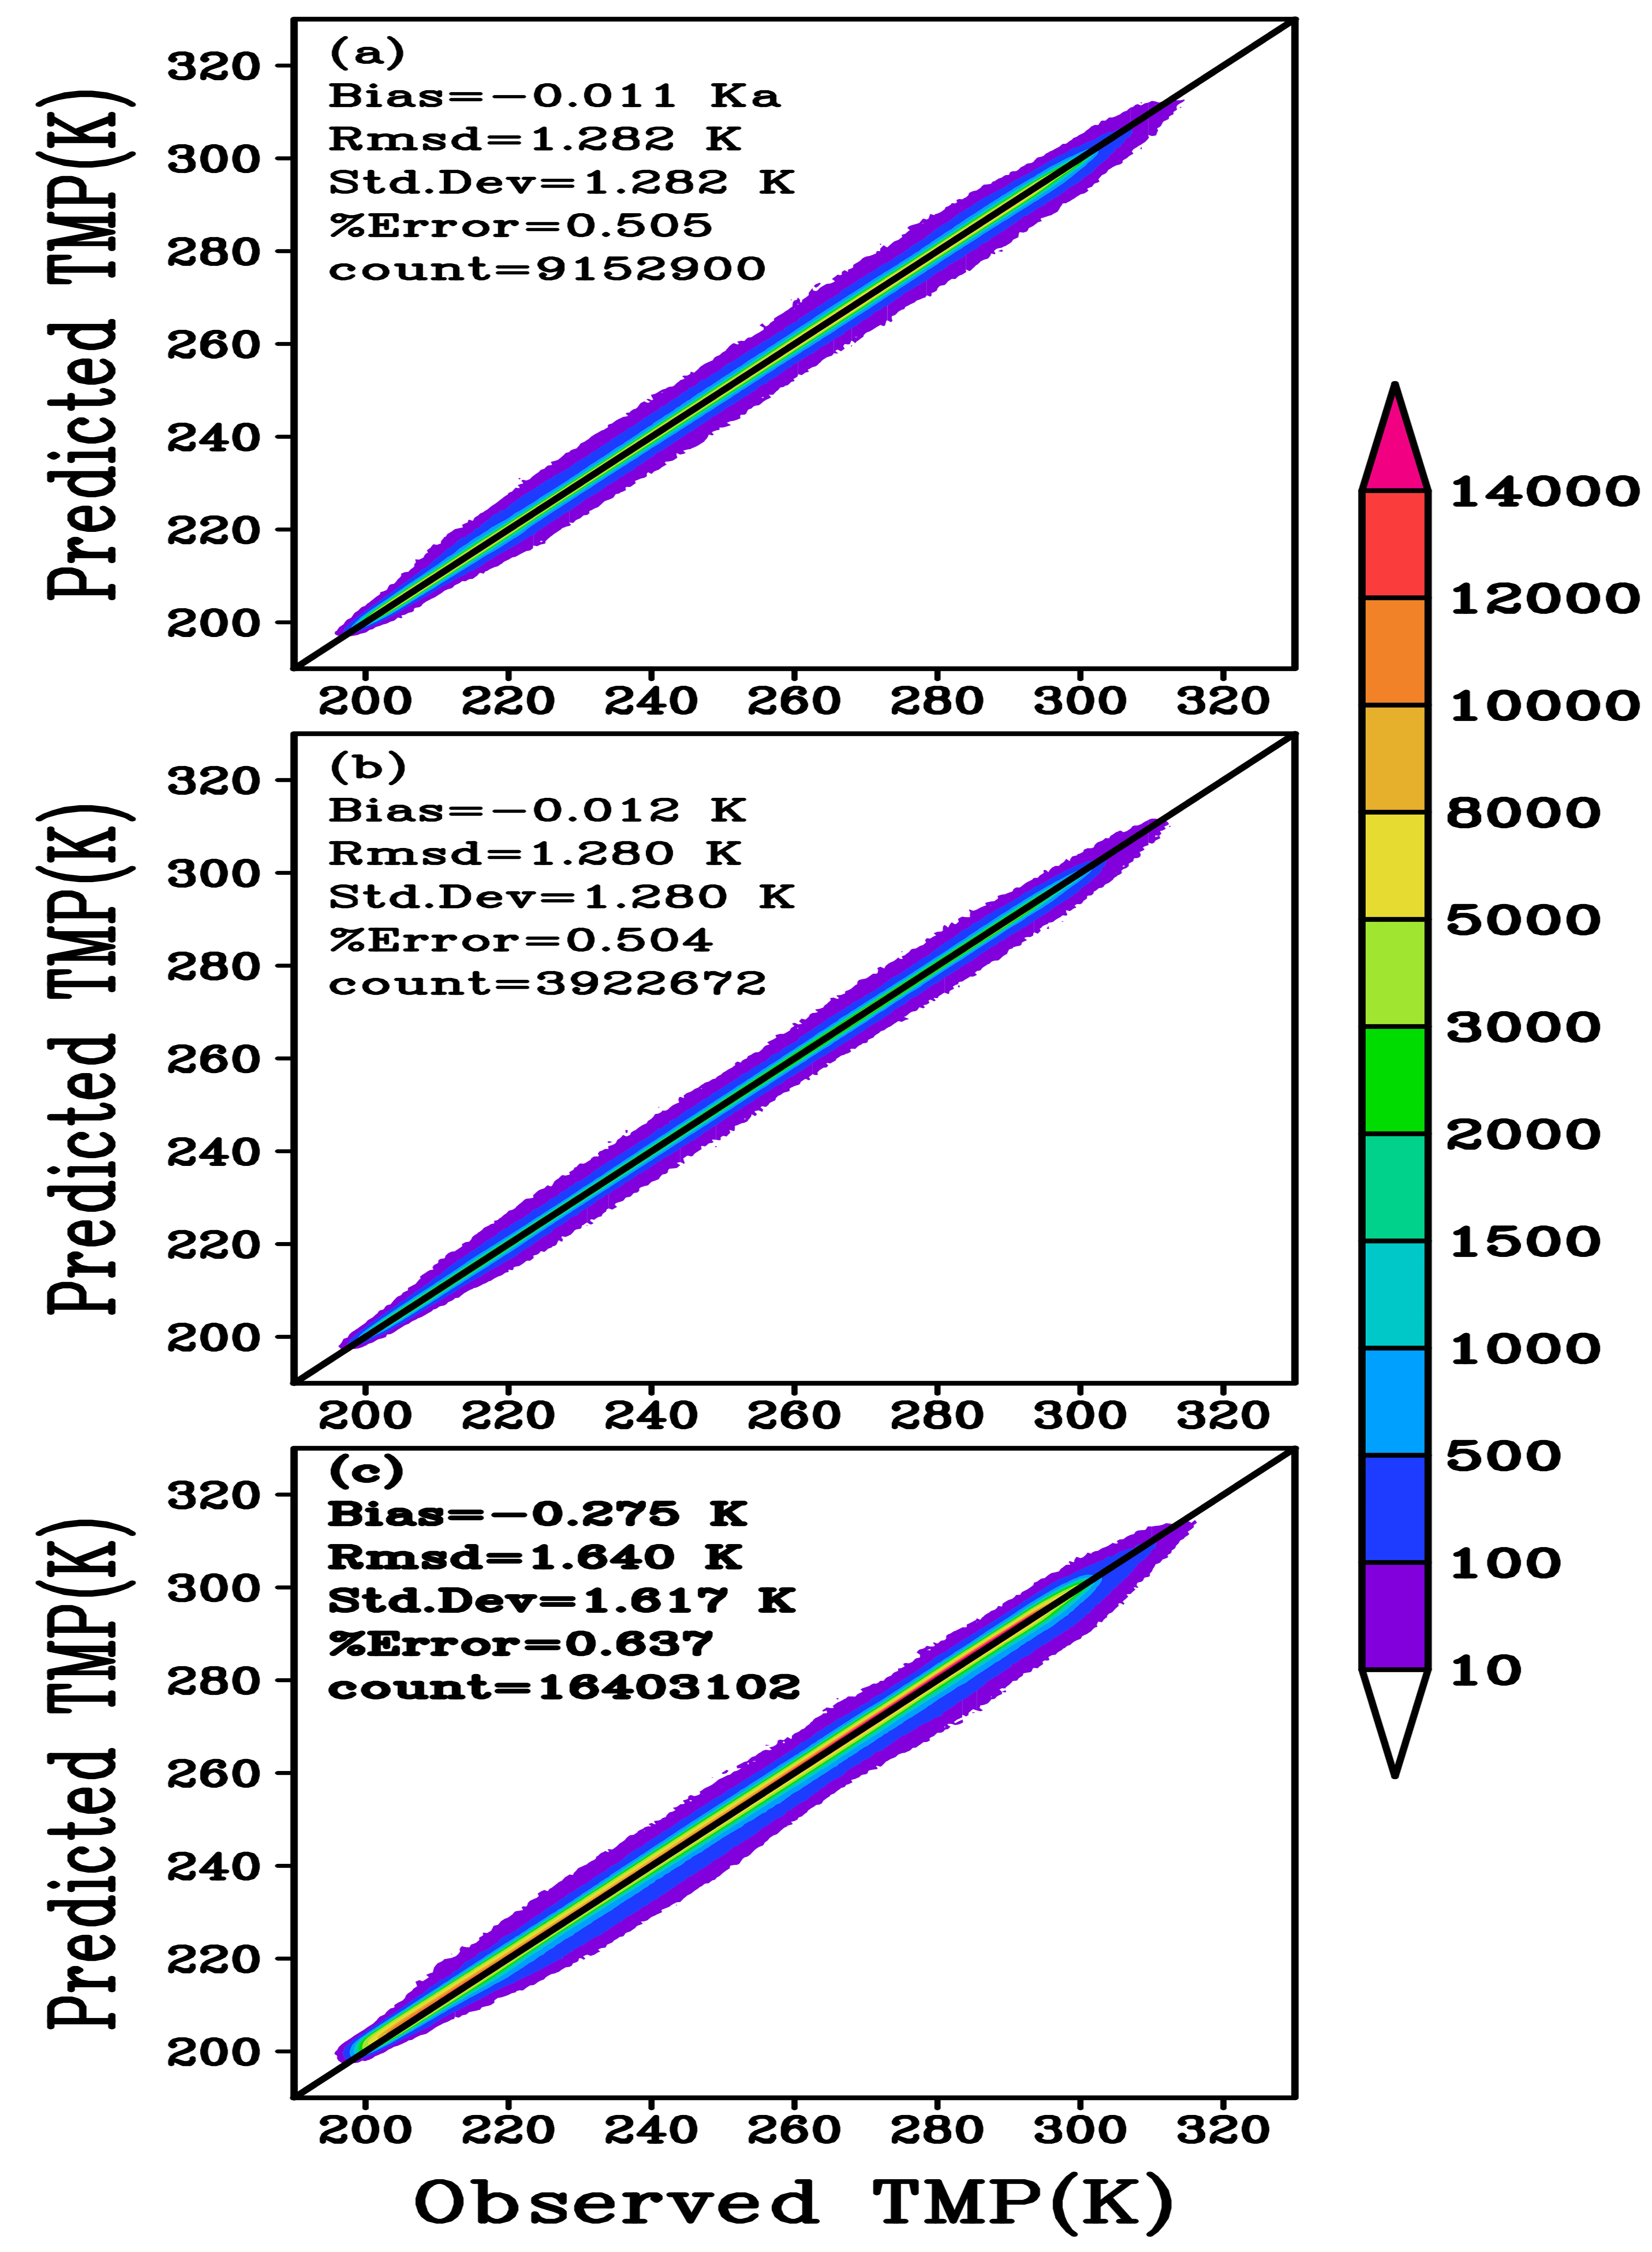
\includegraphics[width=0.7\textwidth, height=12cm]{/Users/soumilhooda/Desktop/COSMIC_REPORT/NEW-FIGURES/scatt-tmp-train20-test20-test21.png}
	\caption{Scatter plot of actual versus retrieved temperature (a) for the training data set in 2020, (b) for testing data set in 2020, and (c) for completely independent data set fot the year 2021. Color bar represents the number of observations available for each temperature bin. This figure is based on data that has been accumulated over all vertical levels and the whole domain.}
	\label{fig:img20}
\end{figure}
\begin{figure}[H]
	\centering
	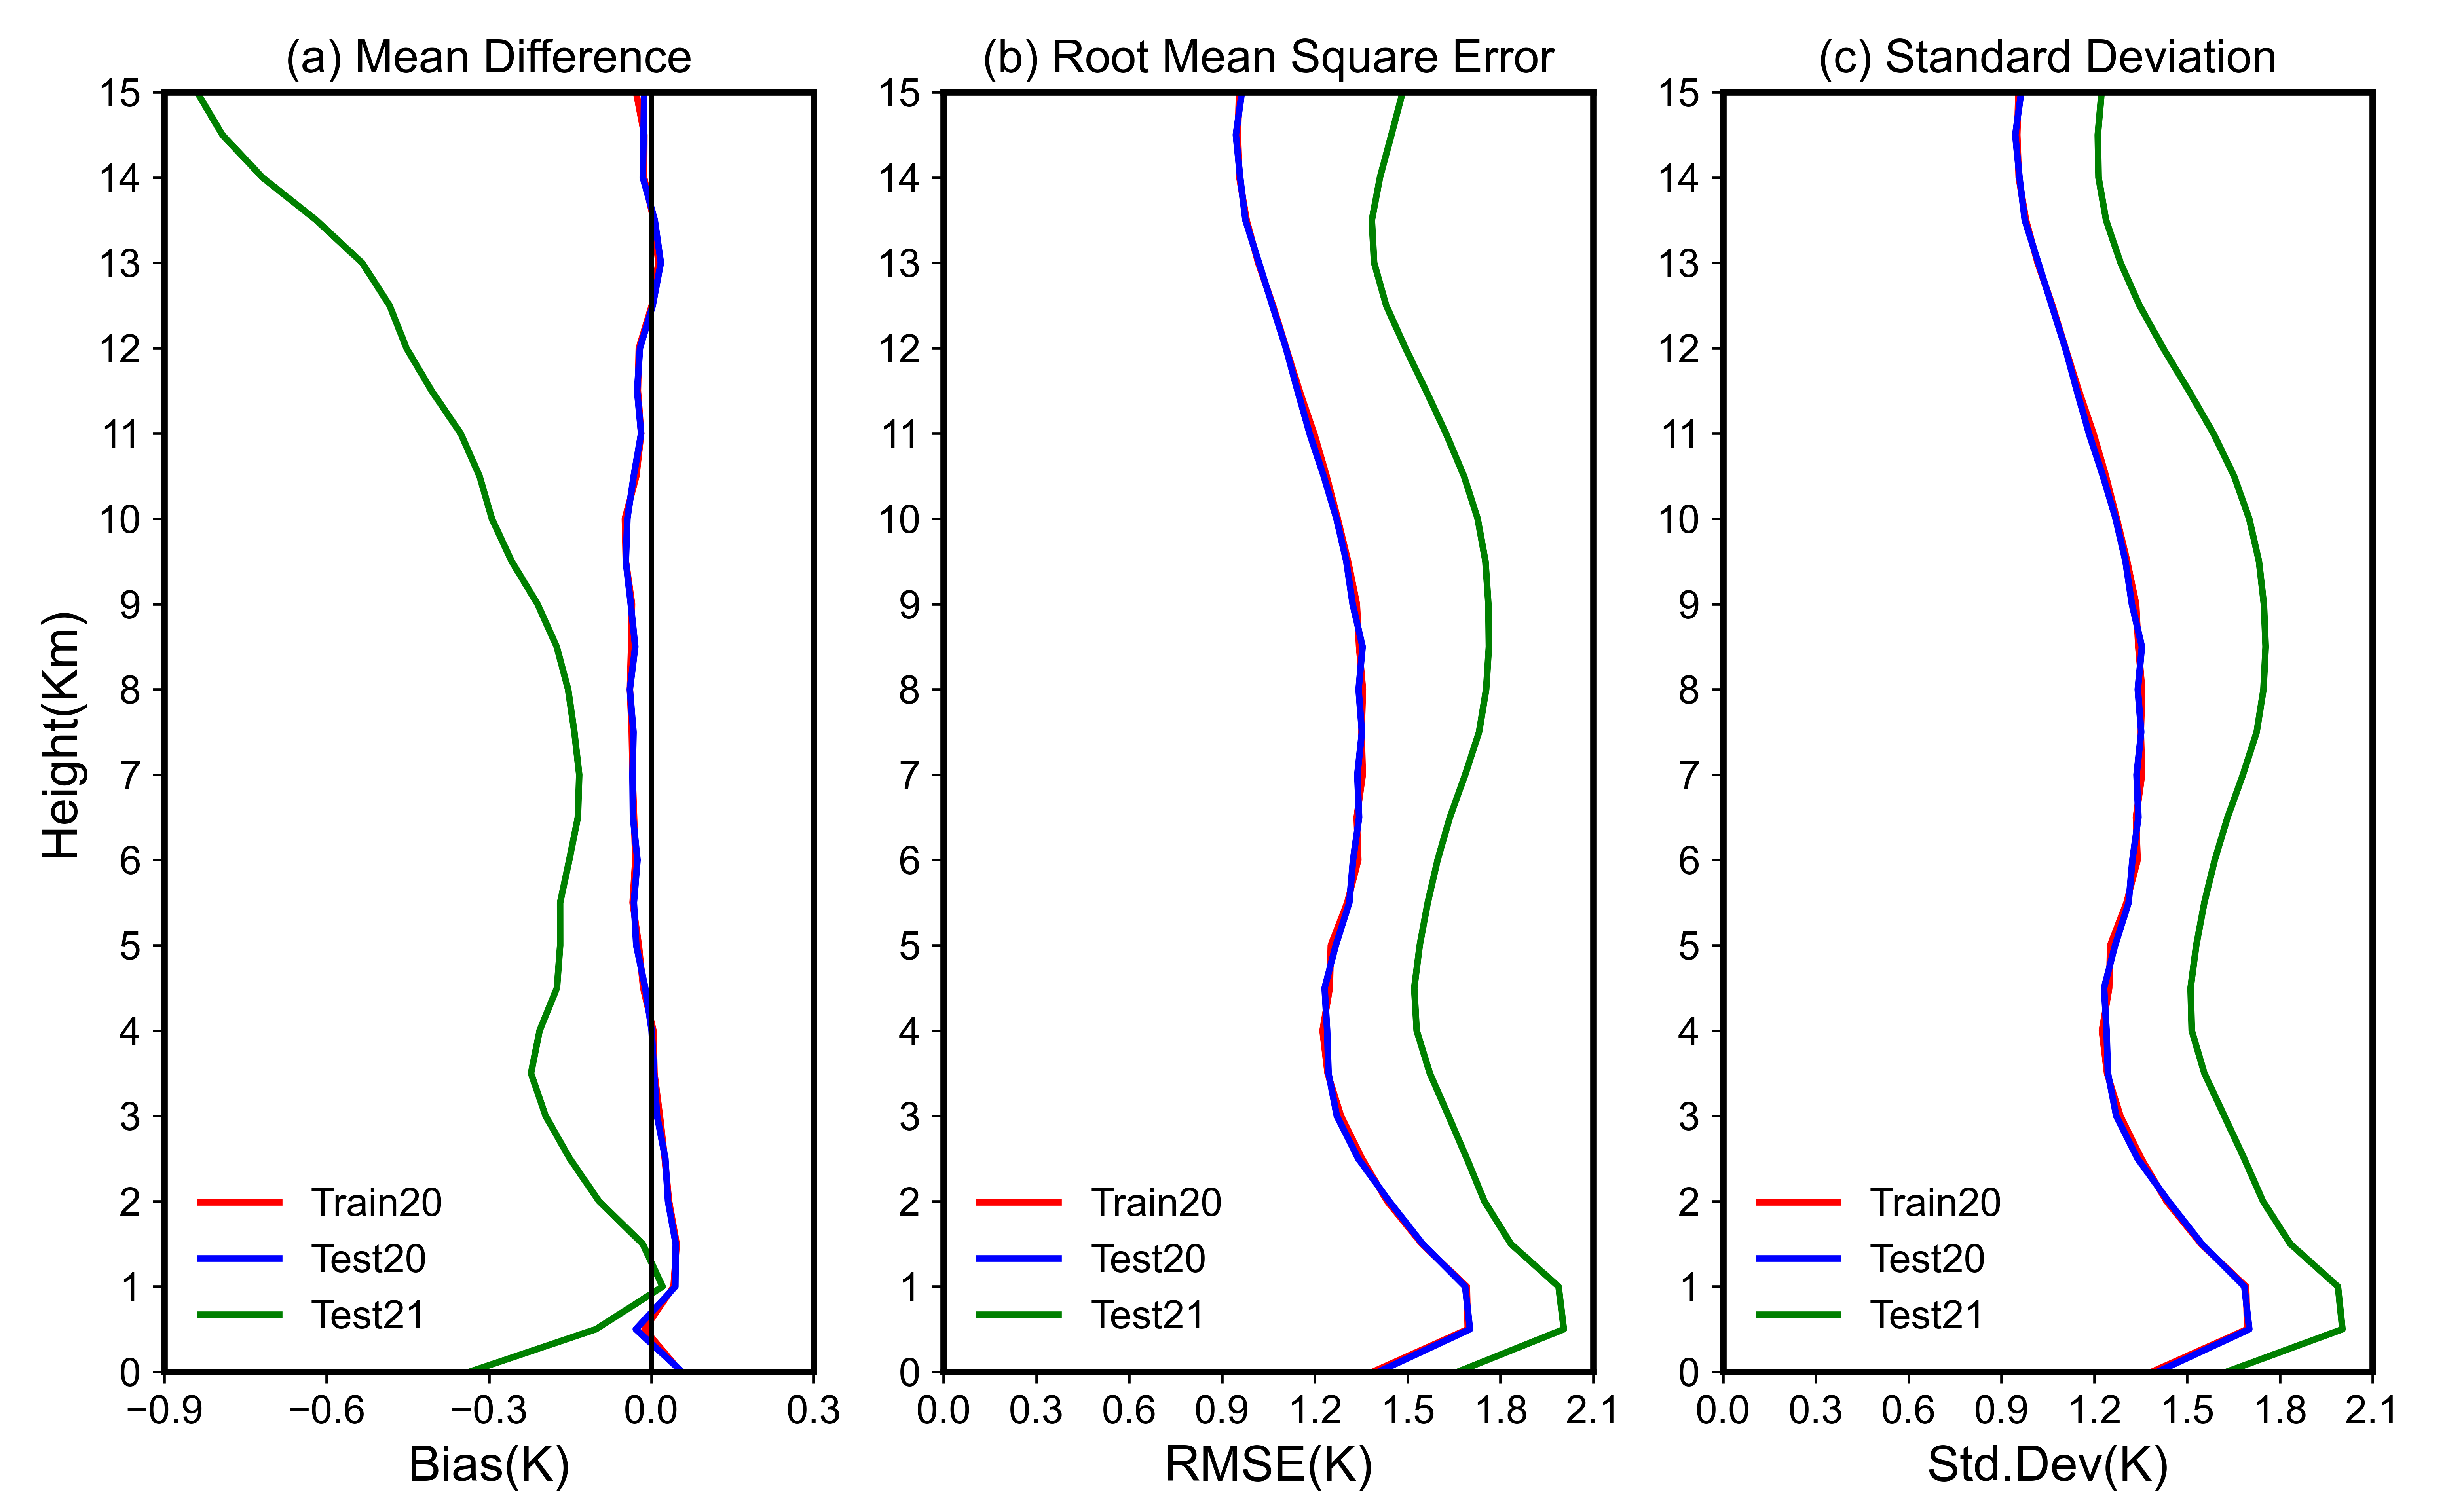
\includegraphics[width=\textwidth, height=7cm ]{/Users/soumilhooda/Desktop/COSMIC_REPORT/NEW-FIGURES/tmp-bias-rmsd-std-profile.png}
\caption{Vertical profiles (a) bias (i.e. mean differences), (b) root mean square error (RMSE), and (c) standard deviation (Std.Dev) of the difference between actual and model retrieved temperature, for training and testing data sets. The data acquired over the entire domain was used to create the figure. }
	\label{fig:img21}
\end{figure}
\begin{figure}[H]
	\centering
	\begin{subfigure}{0.32\textwidth}
		\centering
		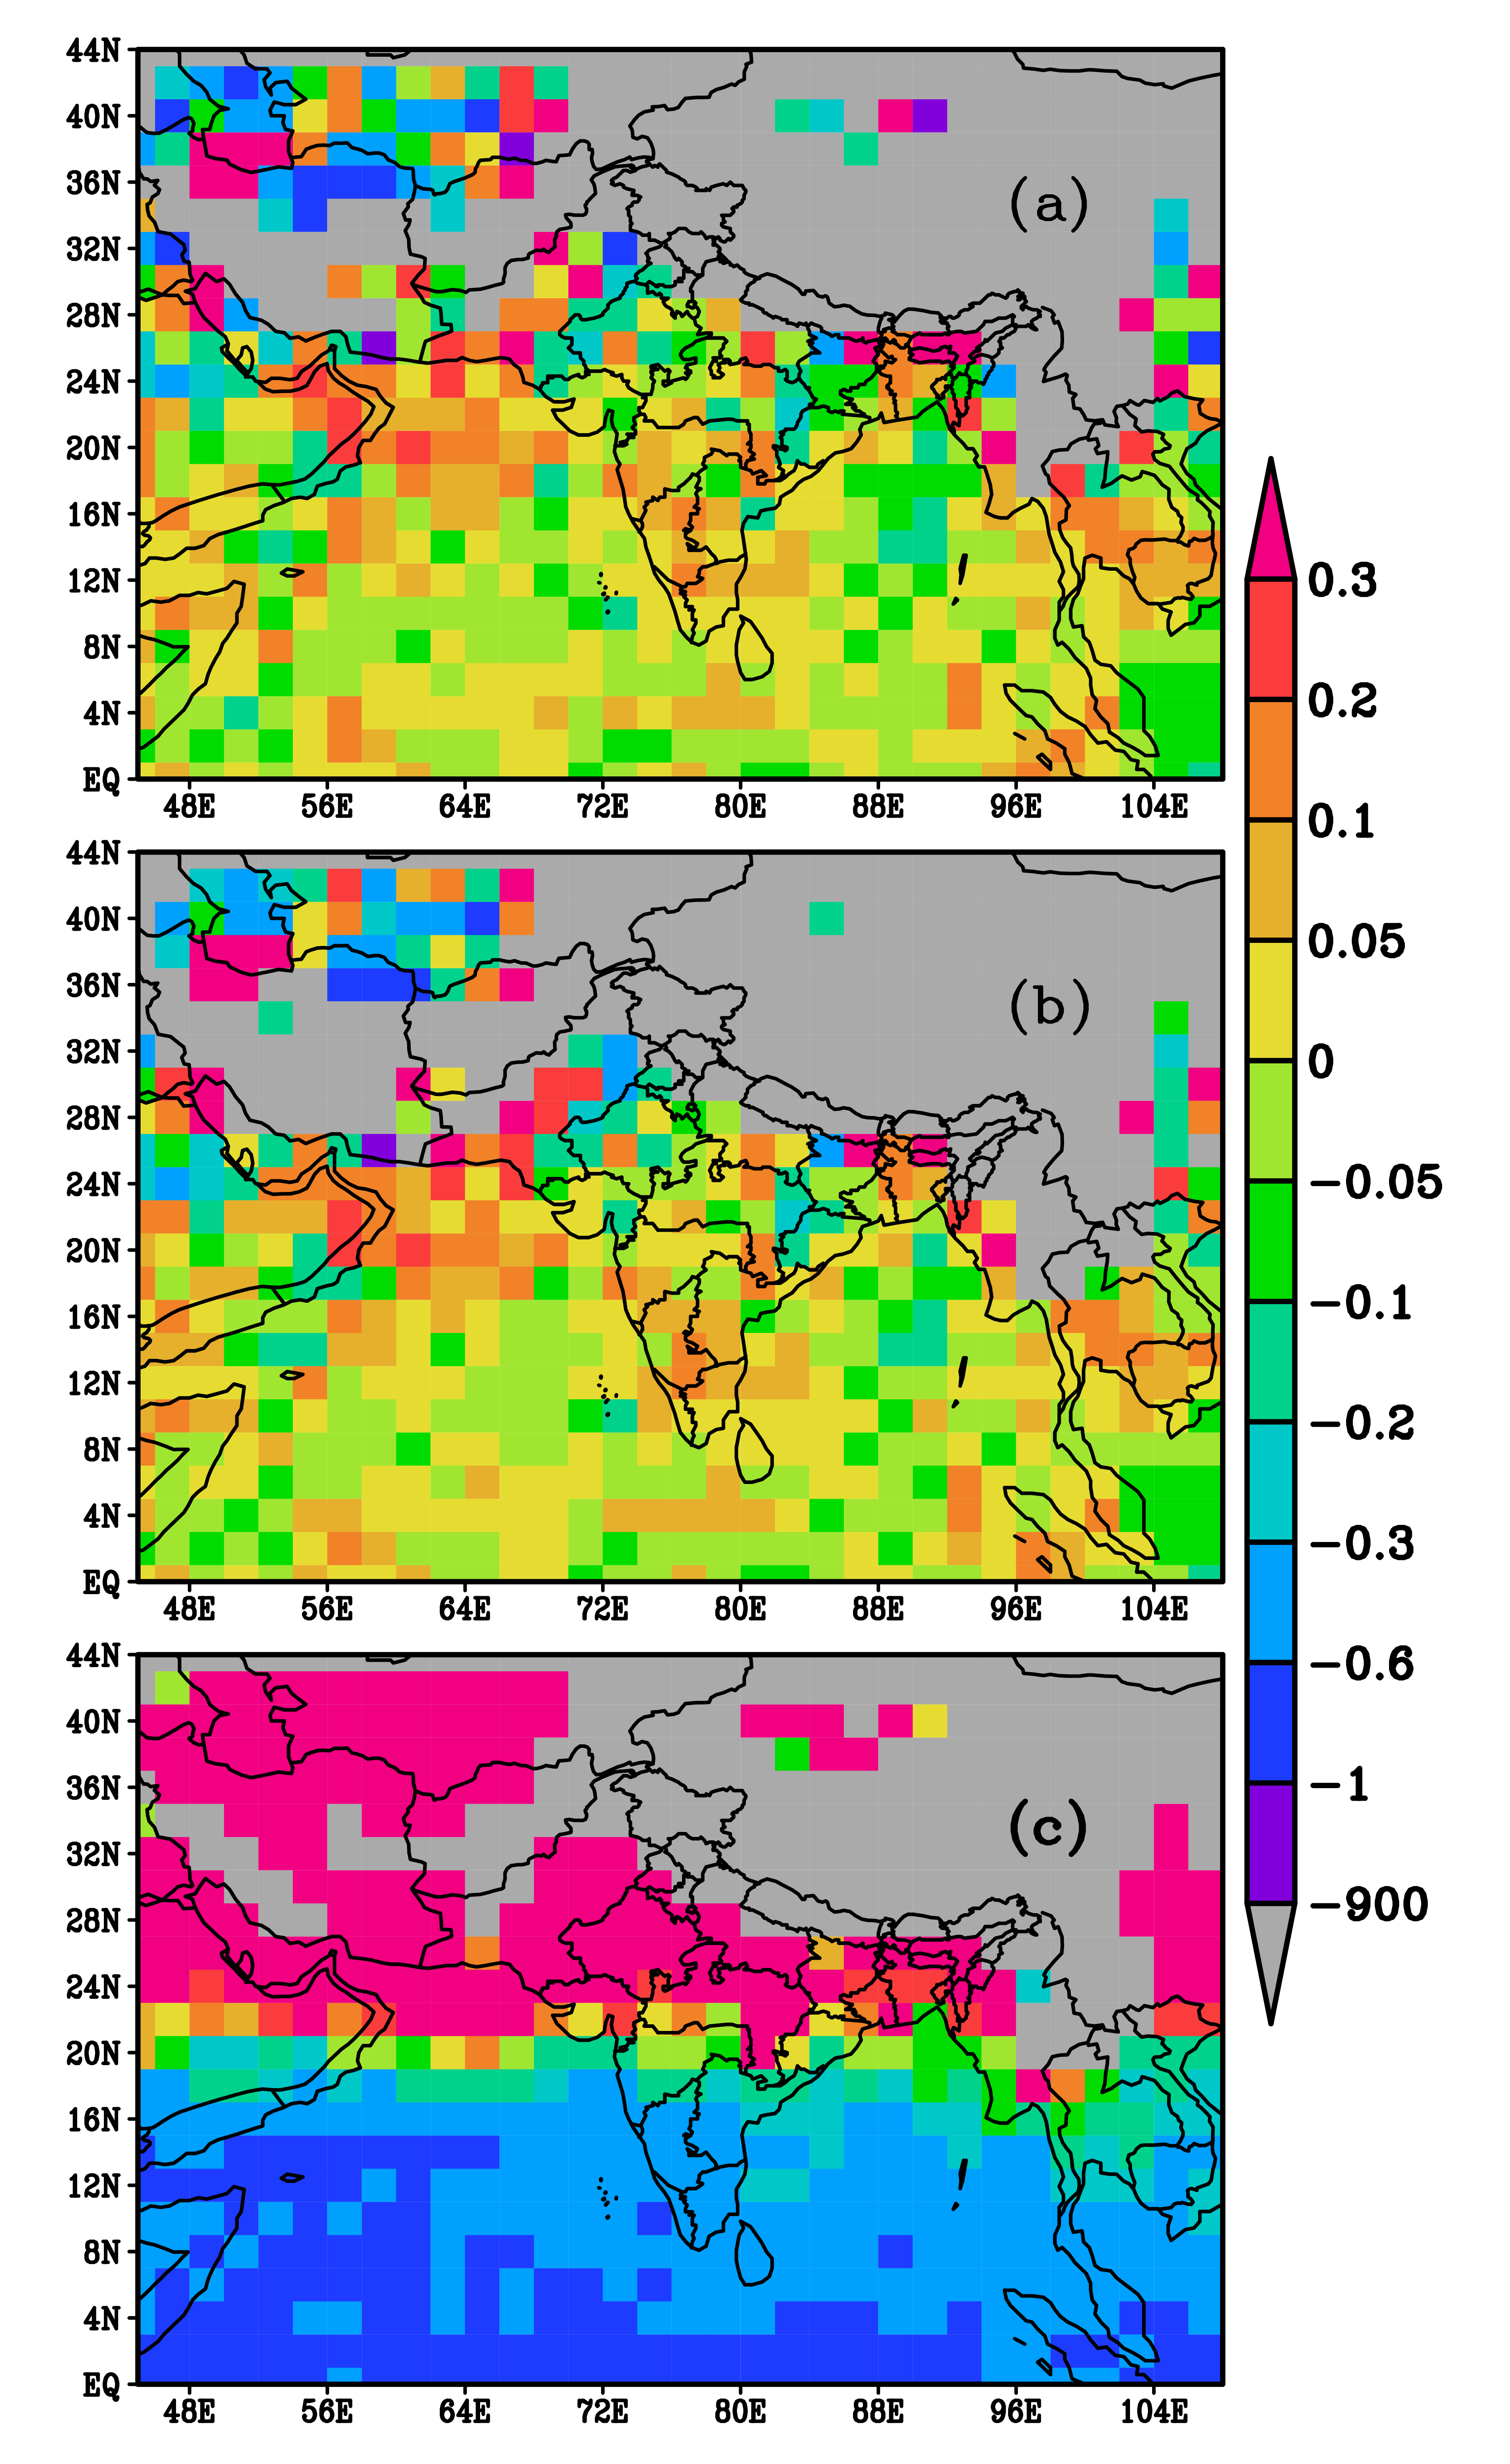
\includegraphics[width=\textwidth, height=9.5cm]{/Users/soumilhooda/Desktop/COSMIC_REPORT/images/dist-tmp-bias-train20-test20-test21.png}
	\end{subfigure}
	\hfill
	\begin{subfigure}{0.32\textwidth}
		\centering
		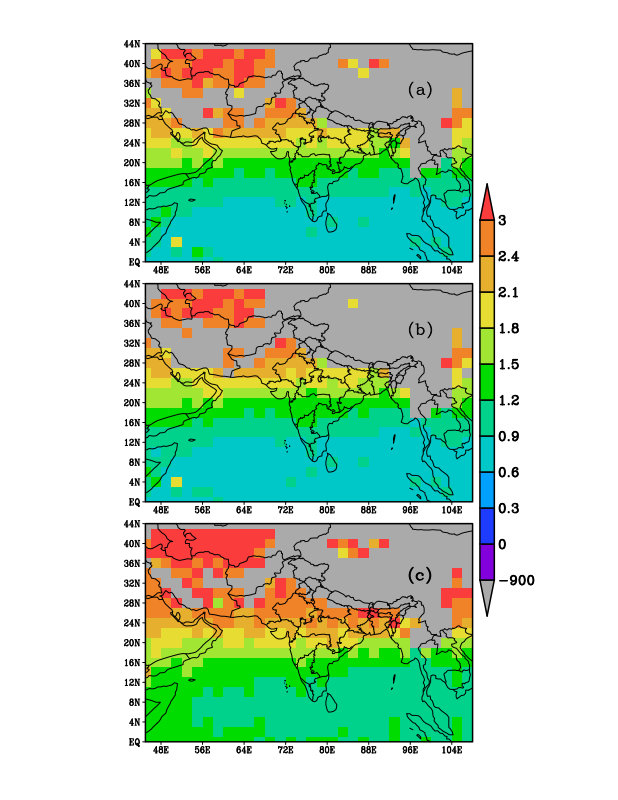
\includegraphics[width=\textwidth, height=9.5cm]{/Users/soumilhooda/Desktop/COSMIC_REPORT/images/dist-tmp-rmsd-train20-test20-test21.png}
	\end{subfigure}
	\hfill
	\begin{subfigure}{0.32\textwidth}
		\centering
		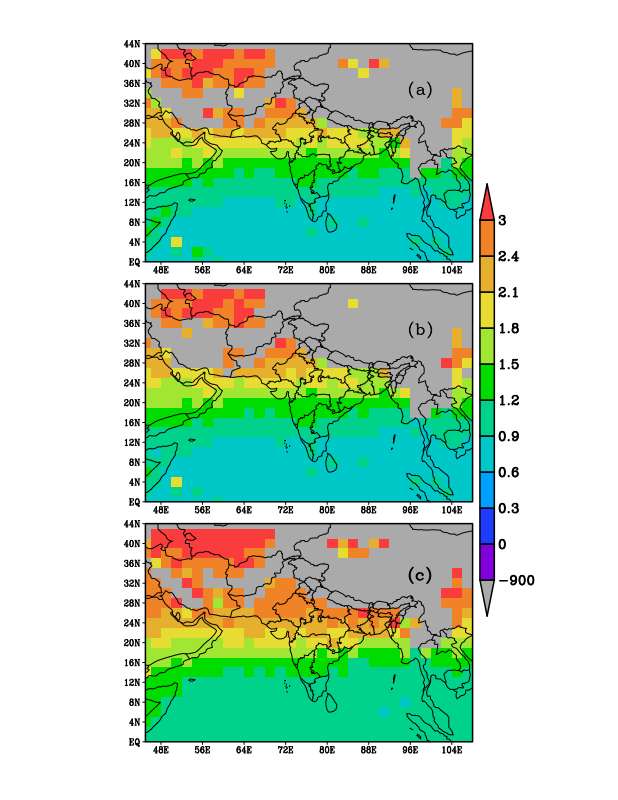
\includegraphics[width=\textwidth, height=9.5cm]{/Users/soumilhooda/Desktop/COSMIC_REPORT/images/dist-tmp-std-train20-test20-test21.png}
	\end{subfigure}
	\caption{Spatial pattern of mean diffferences (i.e.bias), root mean square differences (RMSE) and standard deviation (Std.Dev) of the differences between actual and model retrieved temperature. First column is for bias, second is for RMSE, and third is for standard deviation. Panels (a), (b) and (c) in each column represent the training data set for 2020, testing data for 2020 and the testing data for 2021. The figure is produced using data collected across all heights.}

\label{fig:img13}
\end{figure}

\noindent  The scatter plot between actual and retrieved pressure for the training-testing and independent datasets can be seen in Figure \ref{fig:img23}. For Train20, Test20, and Test21, the retrieved errors are 1.26 hPa, 1.26 hPa, and 1.82 hPa, respectively. The 2020 train and test datasets have very little bias, while the 2021 independent test datasets have a noticeable bias. The vertical profiles for bias, RMSE, and standard deviation are shown in Figure \ref{fig:img24}. The biases are minimal through the troposphere for both the training and testing datasets for the year 2020. However, with the 2021 independent sample, a sizable overestimation is seen in the retrieved profile, with a bias as high as -1.5 to -1.8 hPa. The RMSE varies from 1 hPa to 1.5 hPa for the training and testing data for the year 2020, and retrieval errors decrease as height increases. Except for near the surface, where errors are 2 hPa to 3 hPa, the RMSE for the independent dataset for the year 2021 ranges from 1.5 hPa to 1.8 hPa. Because pressure and refractivity are weakly correlated in the lower troposphere compared to the upper troposphere, there is a larger error in the retrieved pressure at lower levels.  A retrieval error below 2 hPa to 2.5 hPa is tolerable since the surface pressure in the lower levels is highly variable, with a variability of about 10 hPa to 15 hPa. \textit{Lasota} (2021) reported a similar pressure retrieval error. \\

\noindent For the training-testing split (2020) and independent (2021) datasets, Figure \ref{fig:img18} displays the spatial distribution of the bias, RMSE, and standard deviation of the differences between actual and predicted pressure. For the 2020 test, the bias ranges from -0.2 hPa to 0.4 hPa, and for the 2021 test, it ranges from -1.2 hPa to 0.5 hPa. RMSE varies across the domain from 0.6 hPa to 3.3 hPa for the 2020 test and from 1.2 hPa to 3.5 hPa for the 2021 test. For the tests in 2020 and 2021, the standard deviation ranges from 0.6 hPa to 3.1 hPa and from 0.9 hPa to 3.4 hPa, respectively. Similar to the water vapour pressure and temperature retrieval errors, the error in retrieved pressure increases as one moves from lower latitudes to higher latitudes. This is most likely because there is less dependence of refractivity on the thermodynamic profiles in higher latitudes, as well as because the atmospheric conditions are more variable there than in the tropical region. \\

\begin{figure}[H]
	\centering
	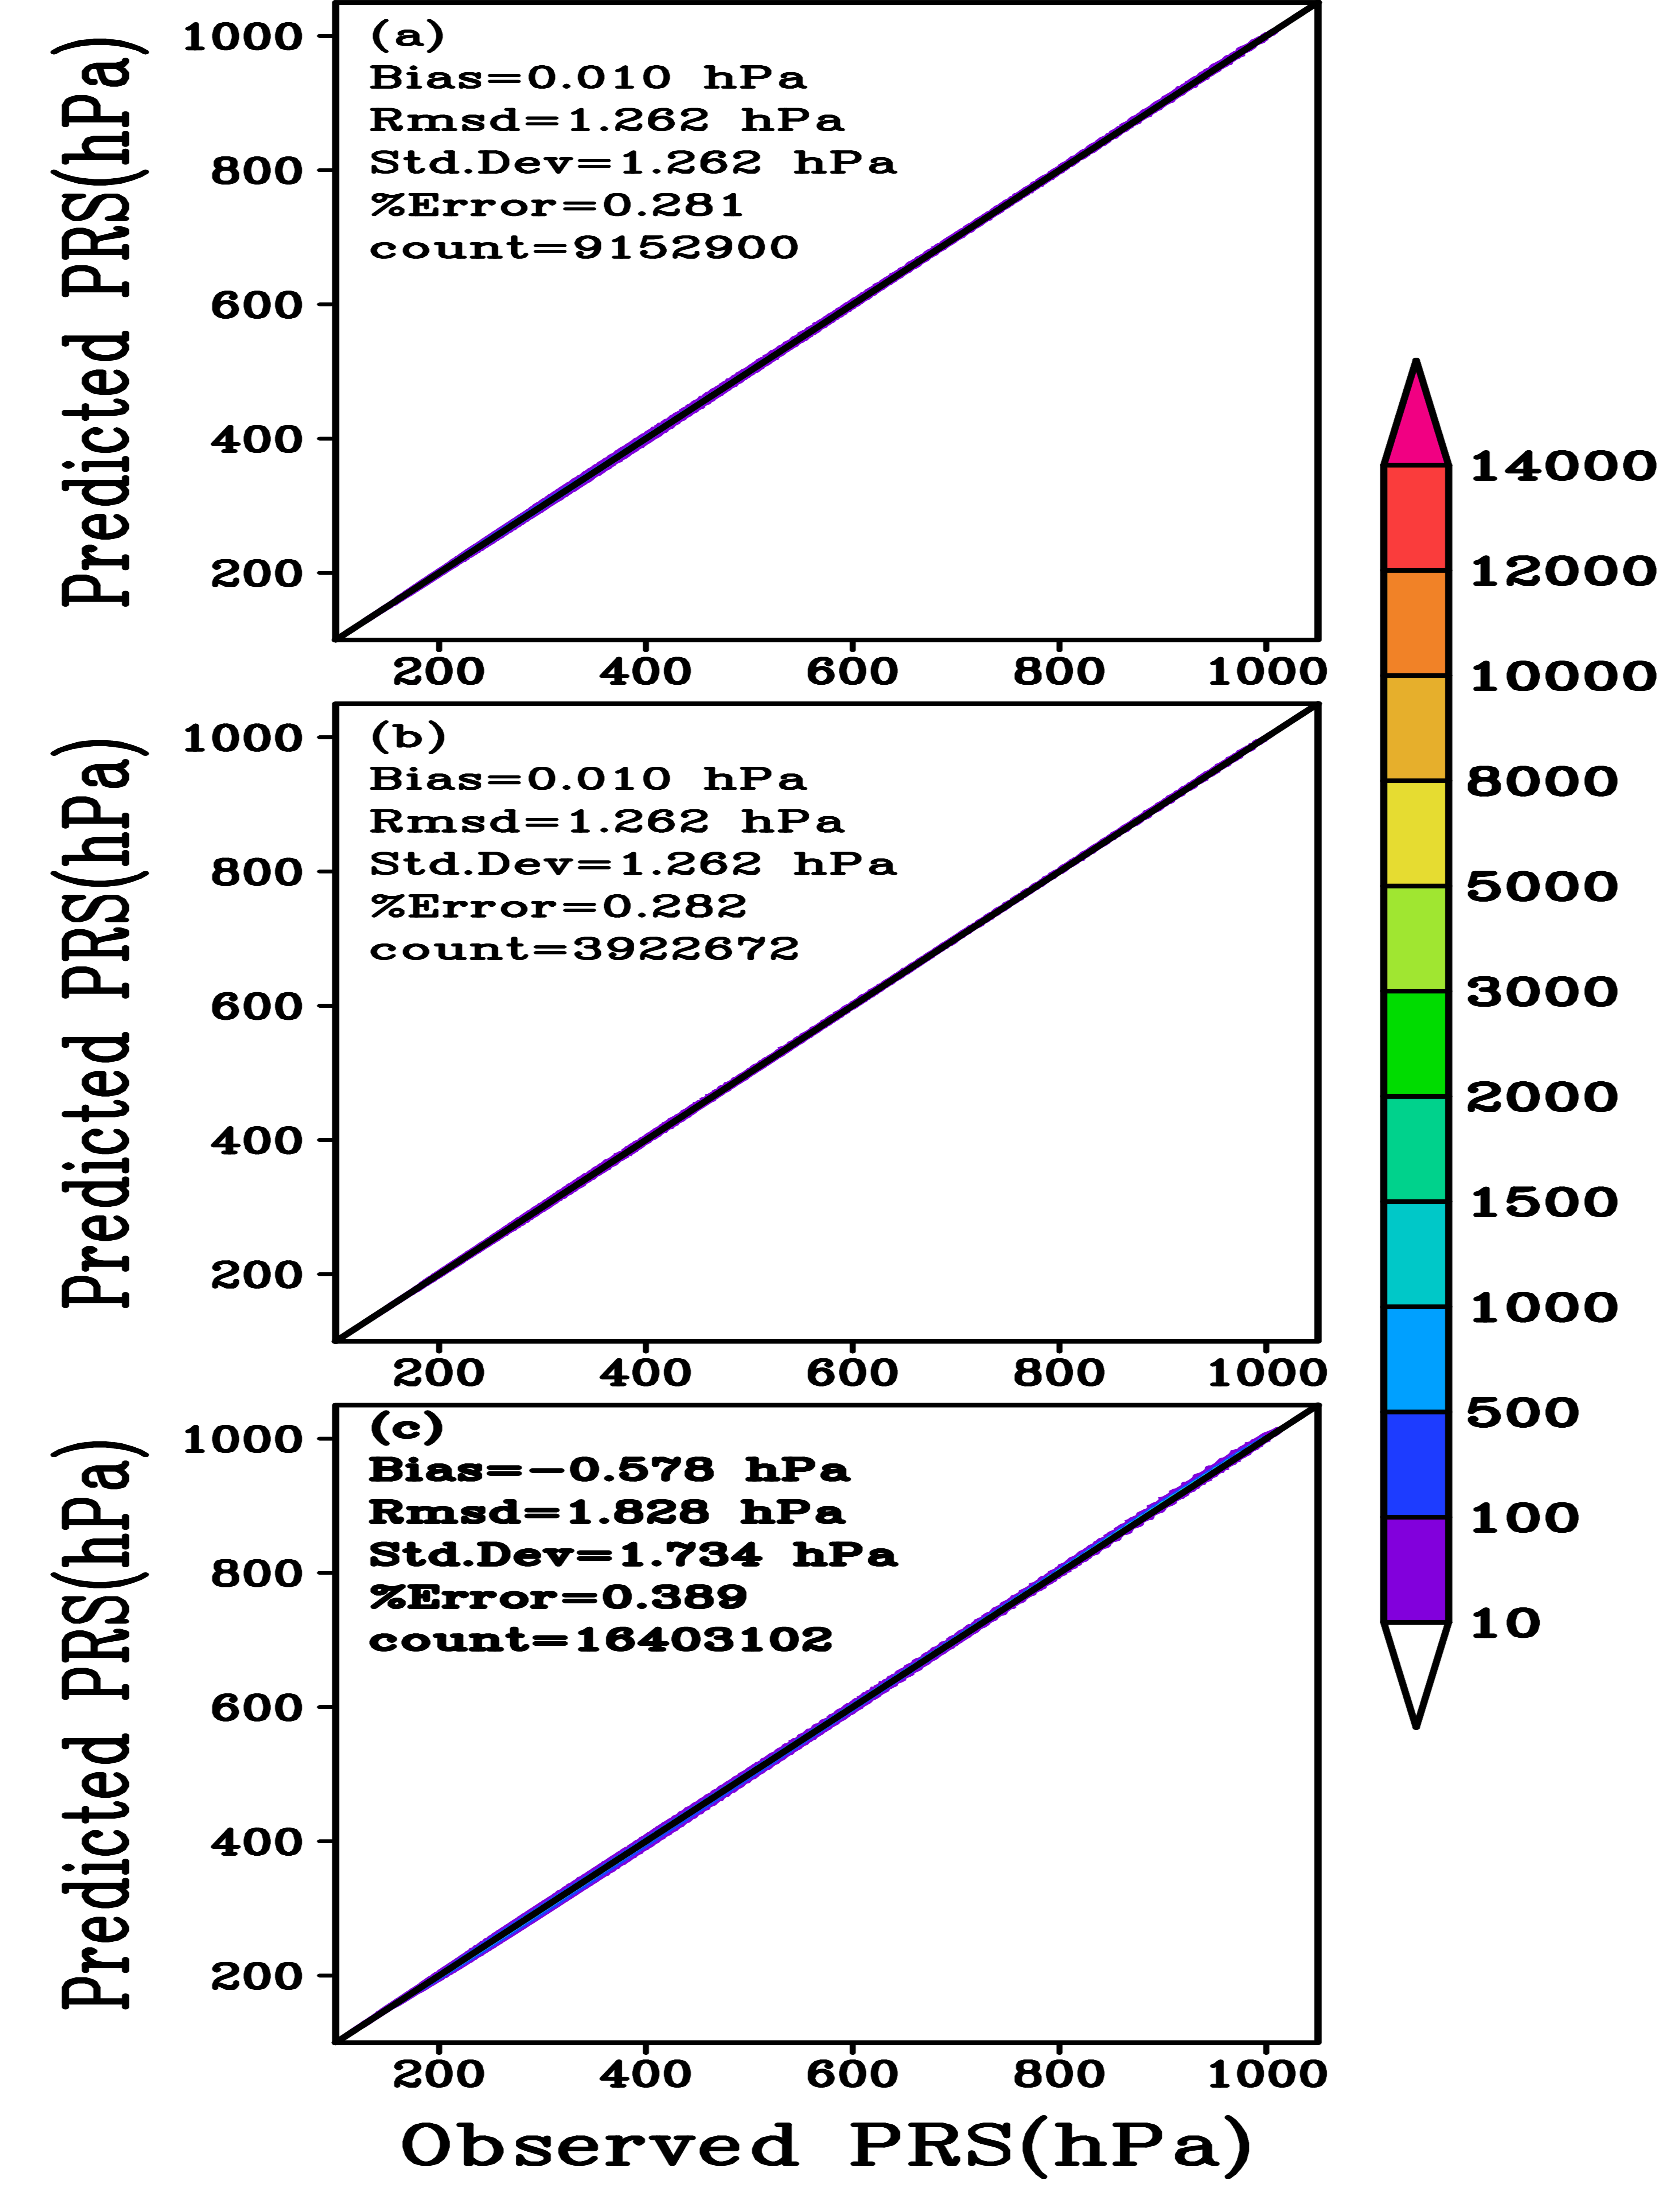
\includegraphics[width=0.7\textwidth, height=12cm]{/Users/soumilhooda/Desktop/COSMIC_REPORT/NEW-FIGURES/scatt-prs-train20-test20-test21.png}
	\caption{Scatter plot of actual versus retrieved pressure (a) for the training data set in 2020, (b) for testing data set in 2020, and (c) for completely independent data set fot the year 2021. Color bar represents the number of observations available for each pressure bin. This figure is based on data that has been accumulated over all vertical levels and the whole domain.}
	\label{fig:img23}
\end{figure}
\begin{figure}[H]
	\centering
	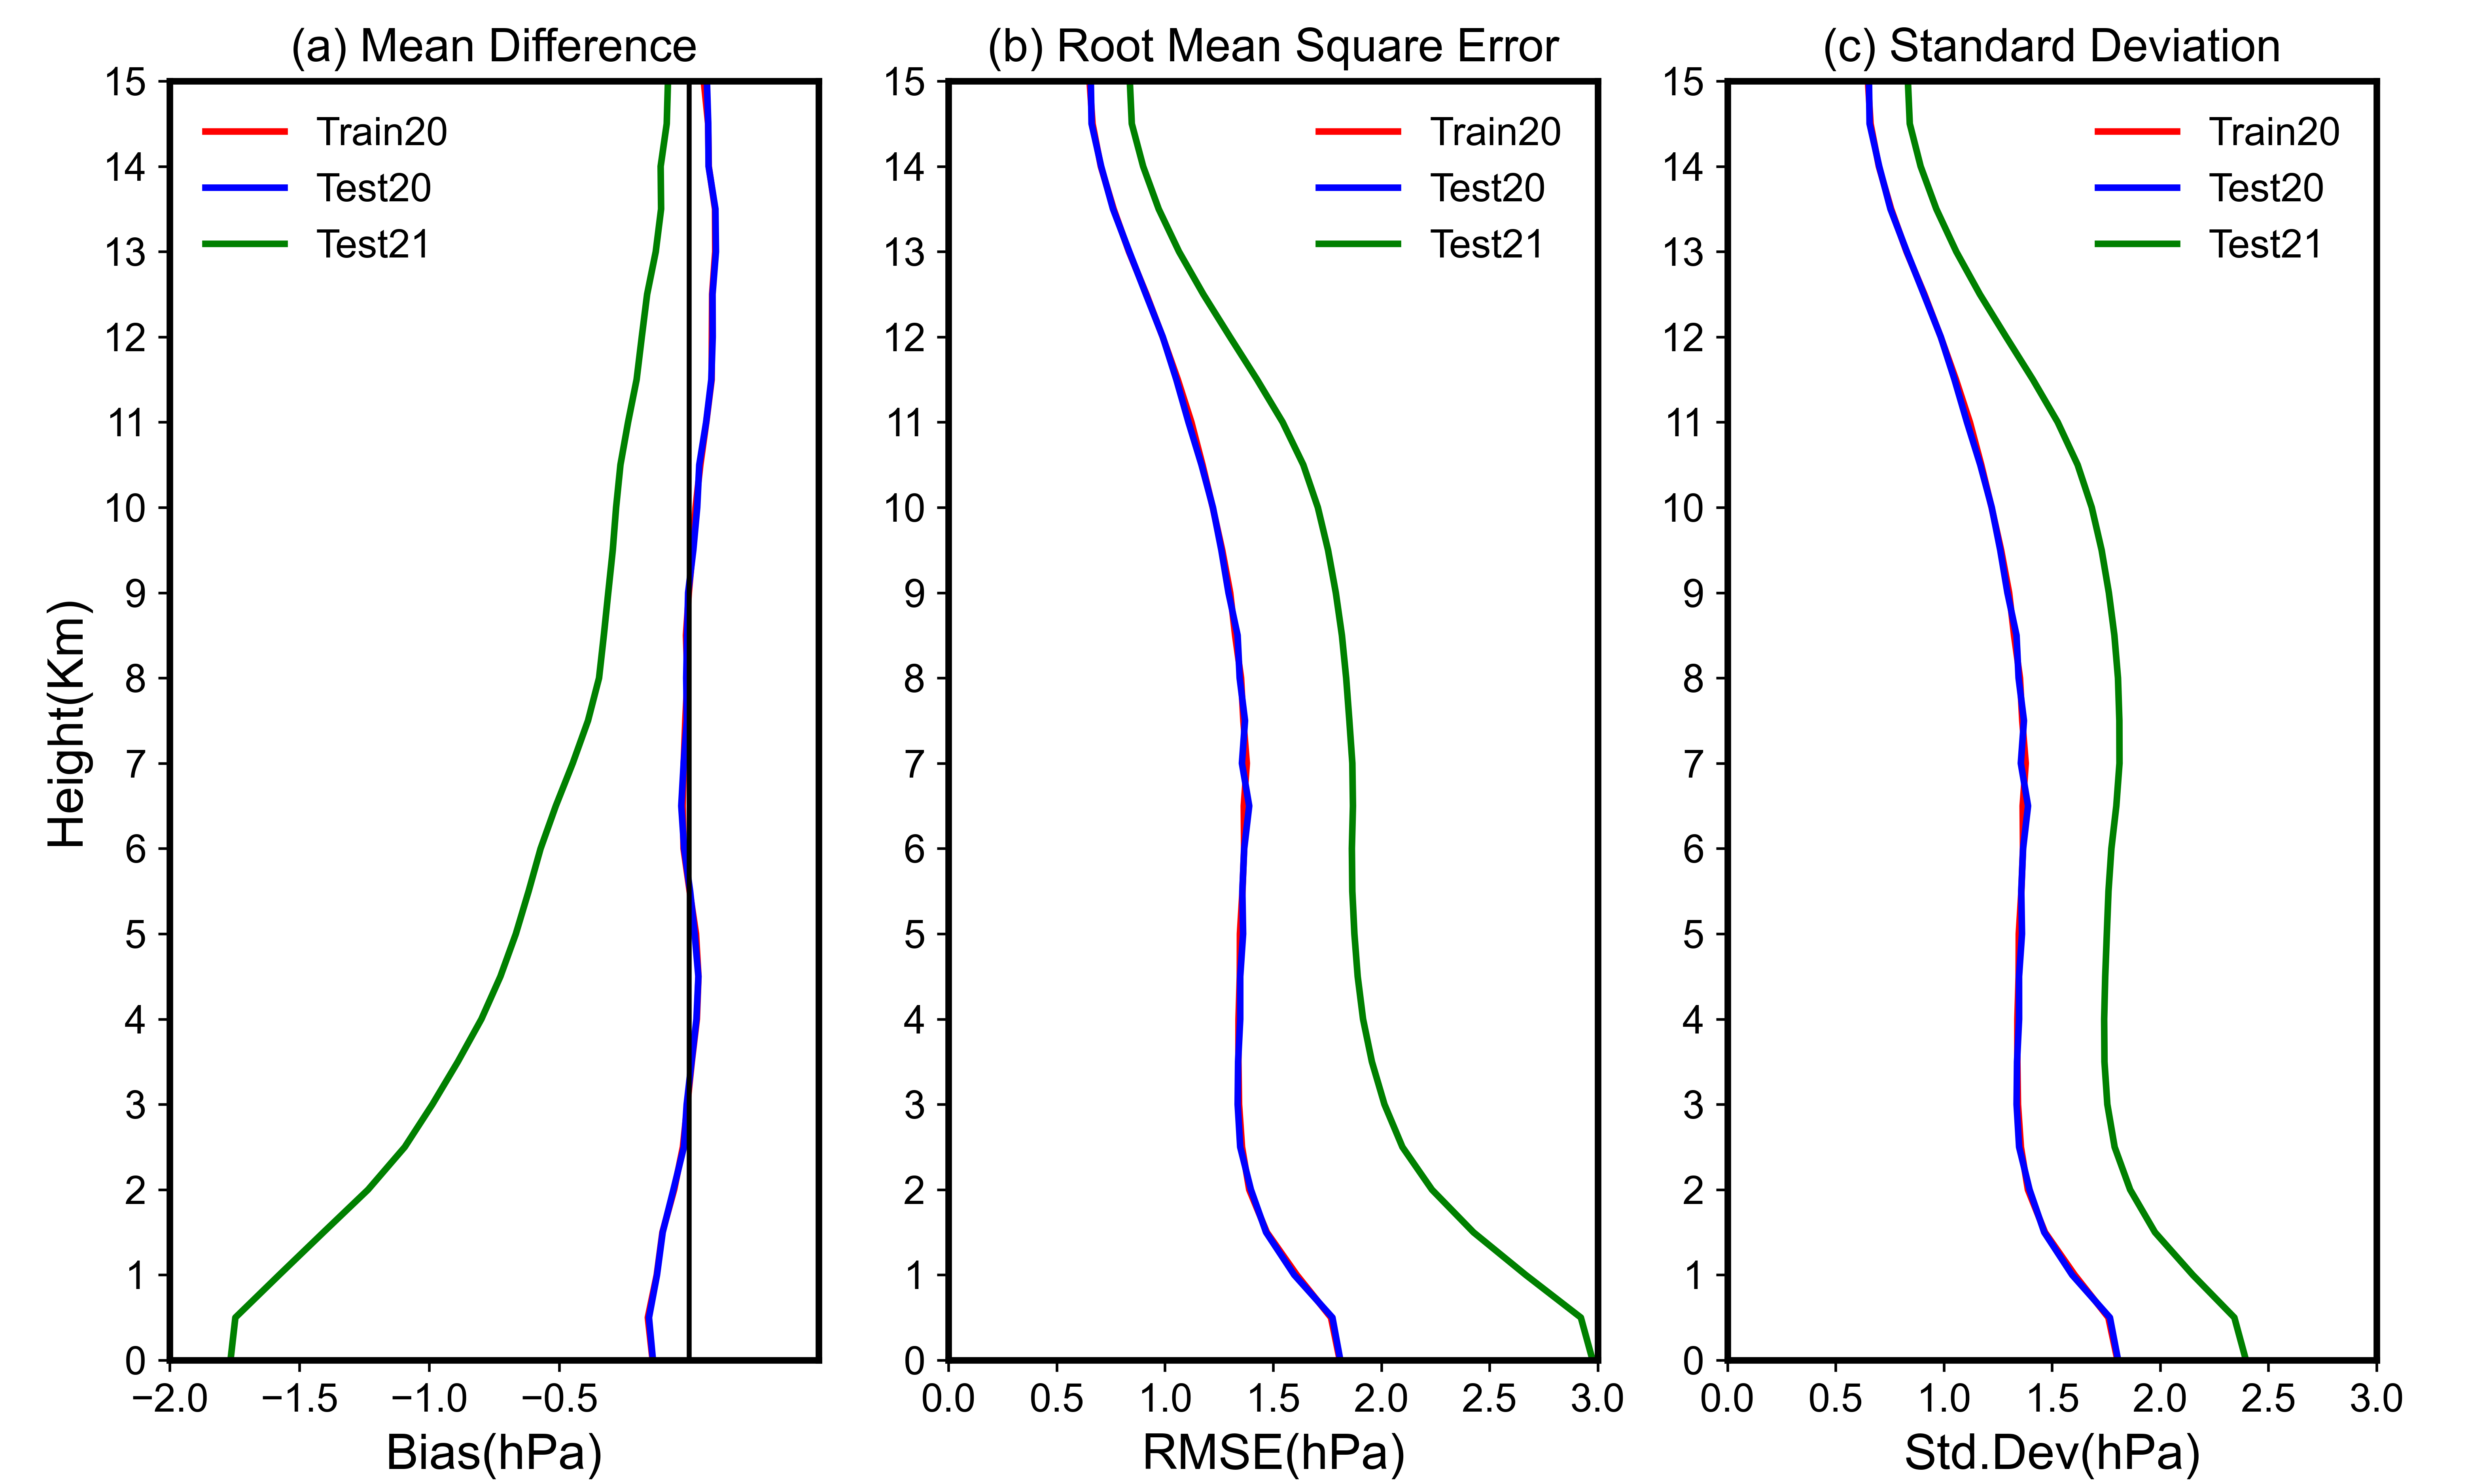
\includegraphics[width=\textwidth, height=7cm ]{/Users/soumilhooda/Desktop/COSMIC_REPORT/NEW-FIGURES/prs-bias-rmsd-std-profile.png}
\caption{Vertical profiles (a) bias (i.e. mean differences), (b) root mean square error (RMSE), and (c) standard deviation (Std.Dev) of the difference between actual and model retrieved pressure, for training and testing data sets. The data acquired over the entire domain was used to create the figure. }
	\label{fig:img24}
\end{figure}
\begin{figure}[H]
	\centering
	\begin{subfigure}{0.32\textwidth}
		\centering
		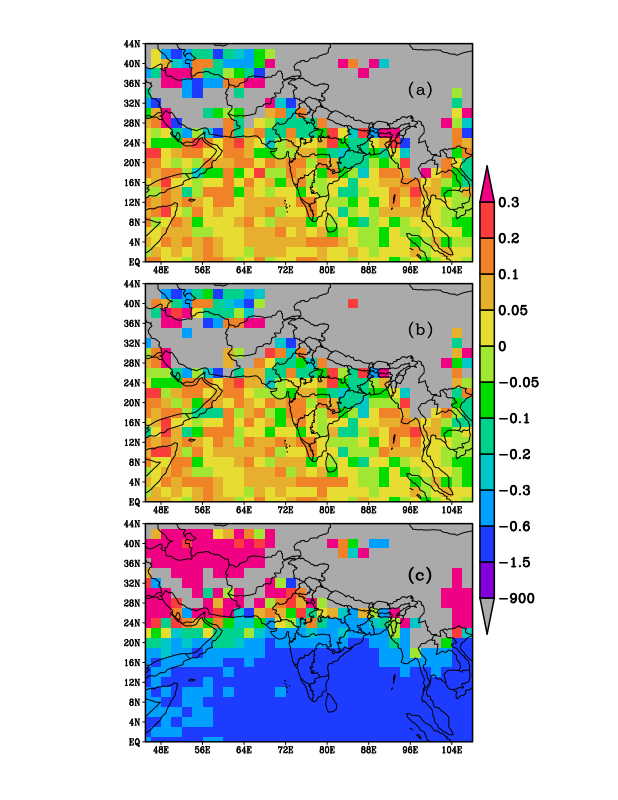
\includegraphics[width=\textwidth, height=9.5cm ]{/Users/soumilhooda/Desktop/COSMIC_REPORT/images/dist-prs-bias-train20-test20-test21.png}
	\end{subfigure}
	\hfill
	\begin{subfigure}{0.32\textwidth}
		\centering
		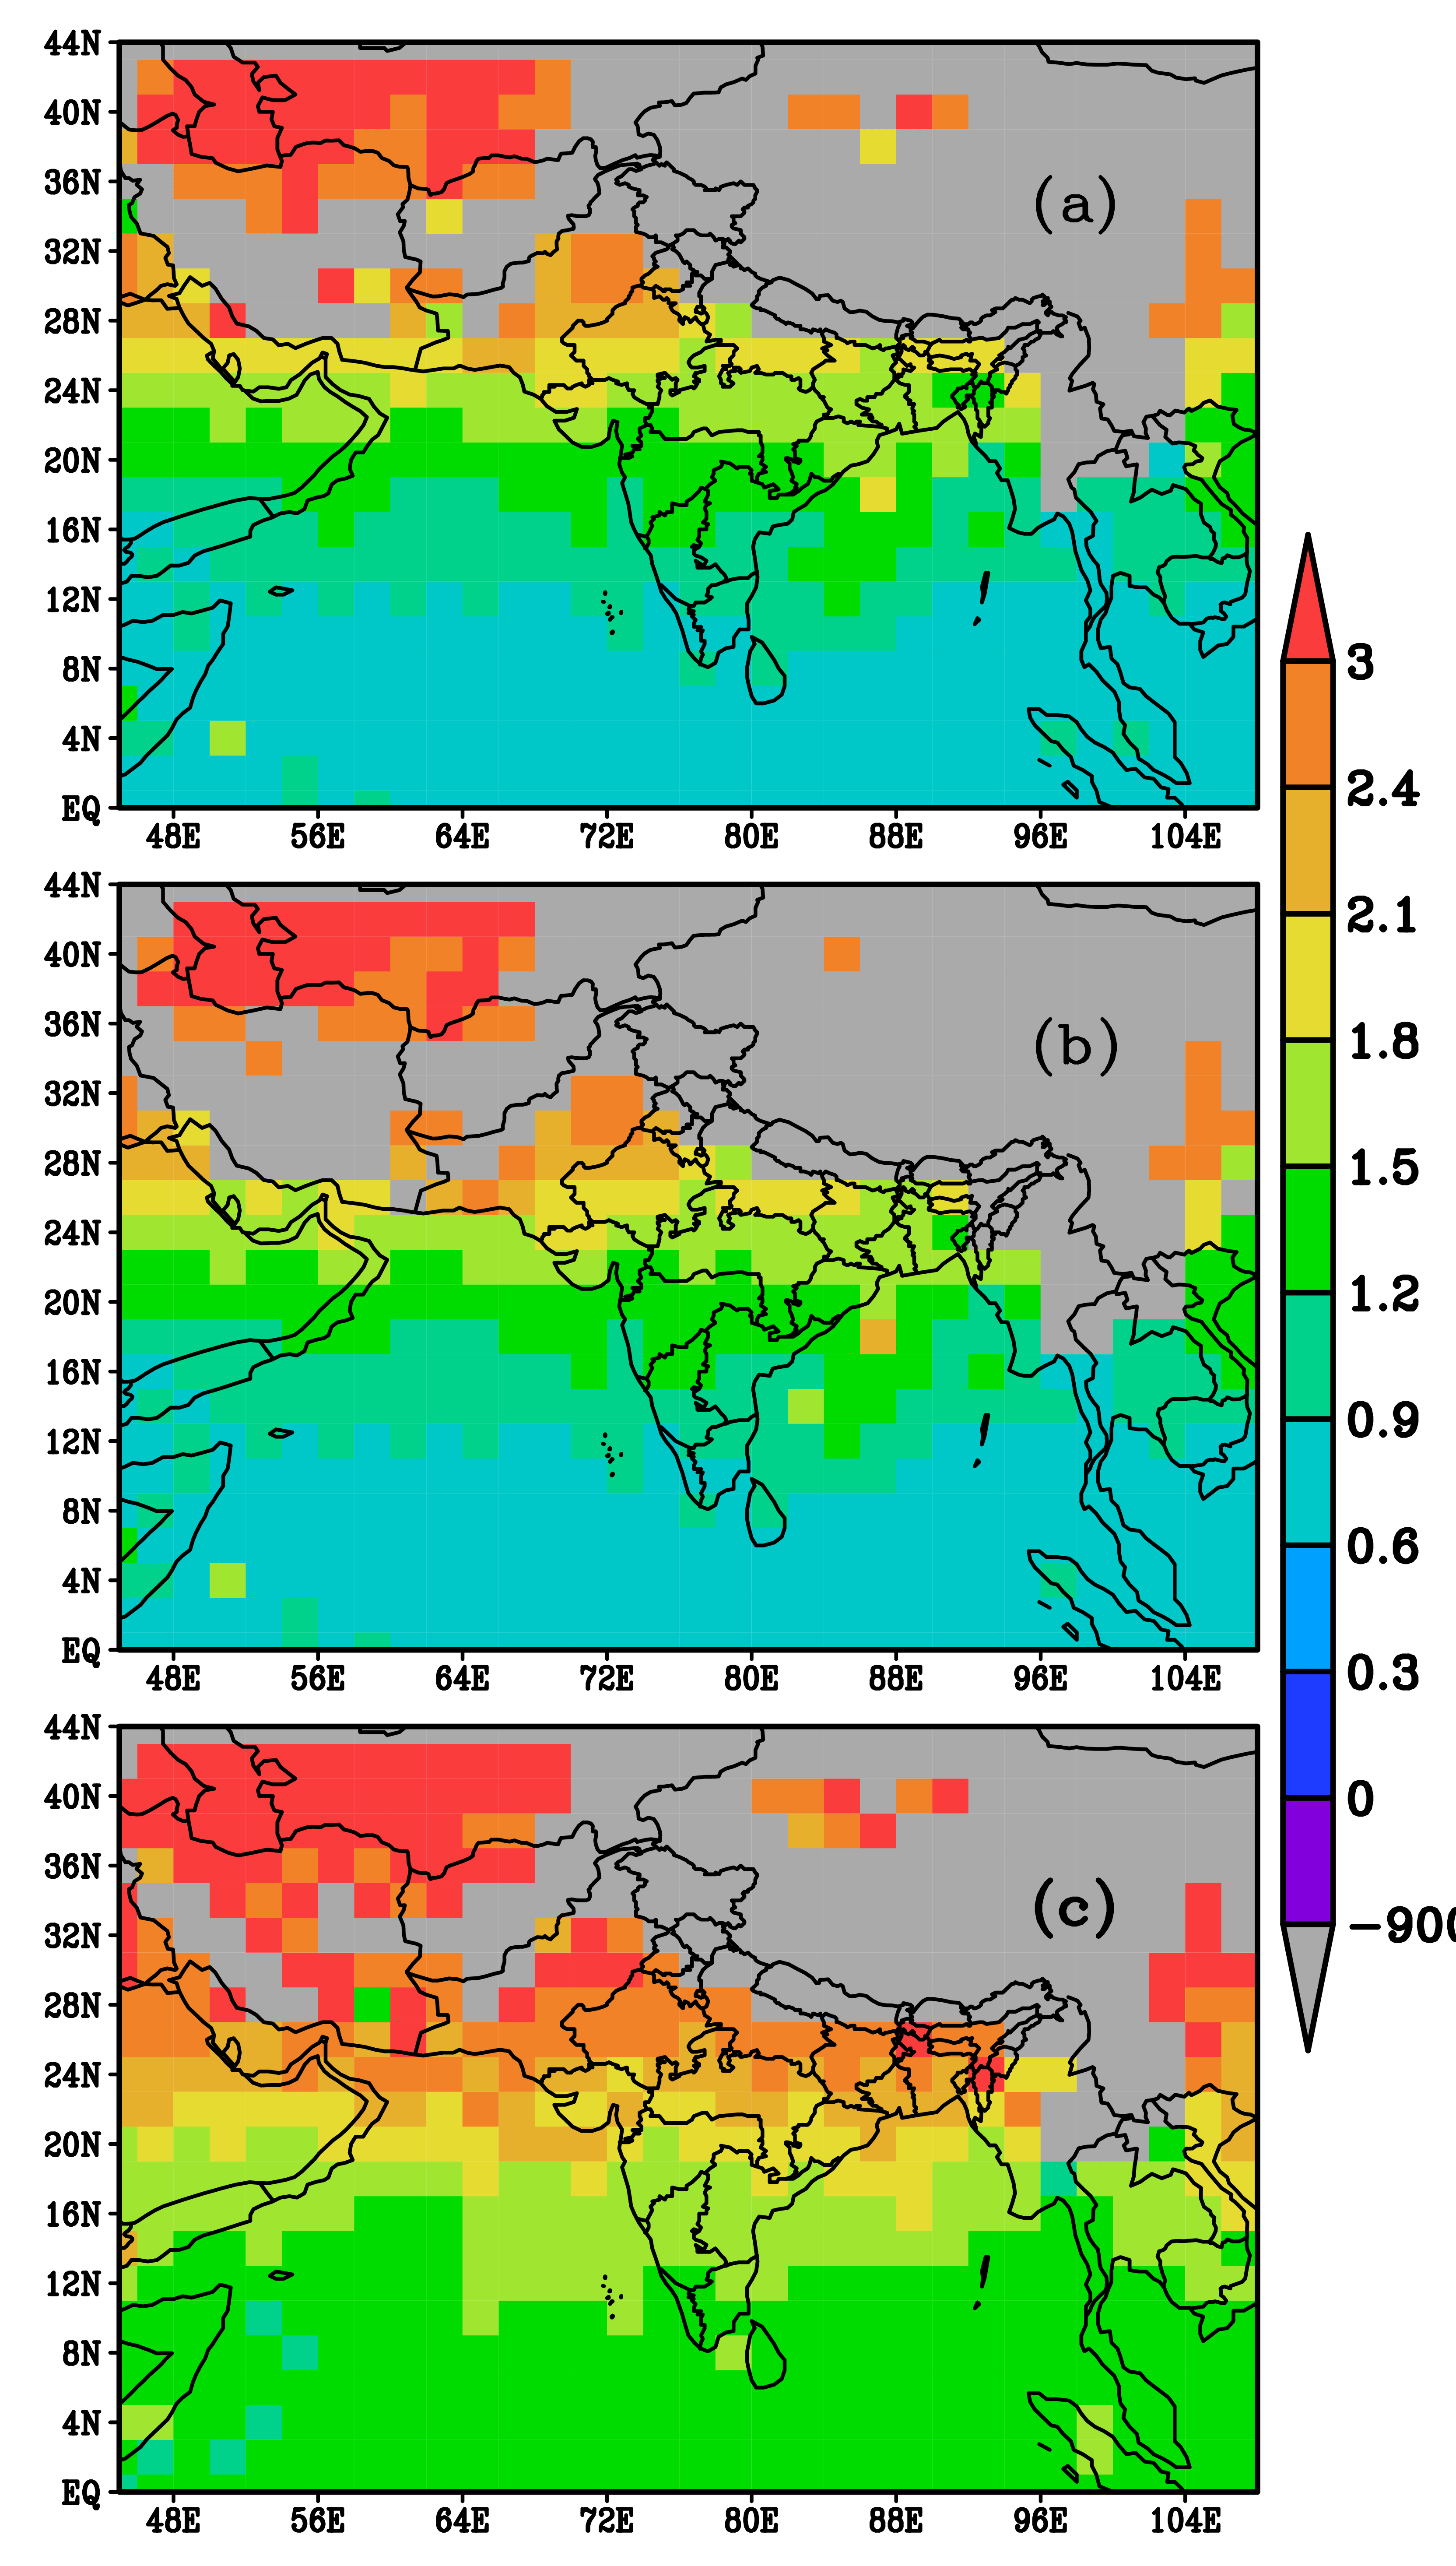
\includegraphics[width=\textwidth, height=9.5cm]{/Users/soumilhooda/Desktop/COSMIC_REPORT/images/dist-prs-rmsd-train20-test20-test21.png}
	\end{subfigure}
	\hfill
	\begin{subfigure}{0.32\textwidth}
		\centering
		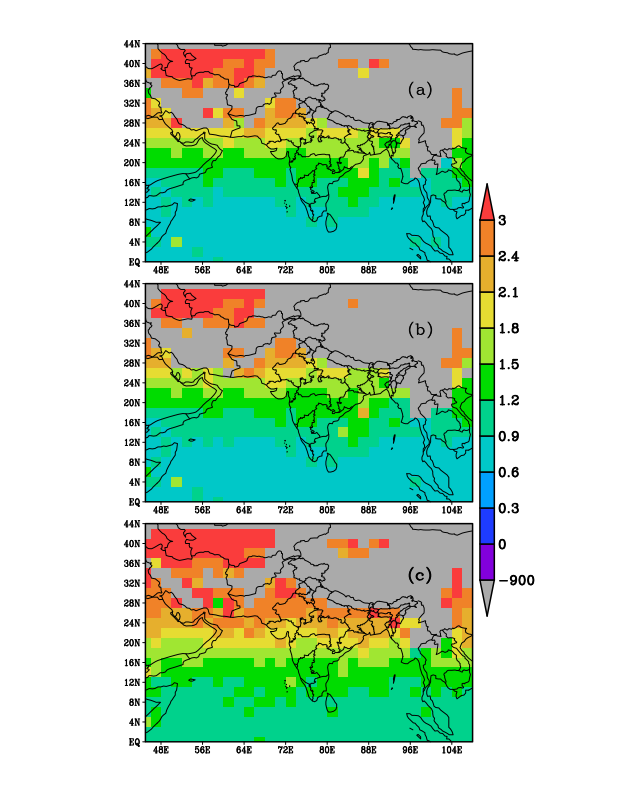
\includegraphics[width=\textwidth, height=9.5cm]{/Users/soumilhooda/Desktop/COSMIC_REPORT/images/dist-prs-std-train20-test20-test21.png}
	\end{subfigure}
	\caption{Spatial pattern of mean diffferences (i.e. bias), root mean square differences (RMSE) and standard deviation (Std.Dev) of the differences between actual and model retrieved pressure. First column is for bias, second is for RMSE, and third is for standard deviation. Panels (a), (b) and (c) in each column represent the training data set for 2020, testing data for 2020 and the testing data for 2021. The figure is produced using data collected across all heights.}

\label{fig:img18}
\end{figure}


\section{Conclusion}

\noindent In order to retrieve thermodynamic profiles from GNSS RO refractivity observations, we performed
this work to develop a reliable system with less need on external data sources. In contrast to earlier
studies, where refractivity and target profiles were taken from two different sources, we used the
simulated data sets for developing the models. This may have avoided additional retrieval errors
caused by errors made during the spatial and temporal collocation of input and output targets. As
far as these added errors are concerned, the simulated observations have an advantage. \\

\noindent In order to retrieve tropospheric thermodynamic profiles from simulated refractivity profiles, two
artificial neural network models were developed. Data from the two-year period of January 2020 to
December 2021 was used in this process. While data from the year 2020 were utilized for developing
and testing the proposed model, data from the year 2021 were used as a completely independent
dataset to check the robustness of the model. On both, the testing dataset and the dataset that was
completely independent, the developed model consistently delivered satisfactory results. When
averaged vertically, the roots mean square errors (RMSE) for temperature, pressure, and water
vapour pressure are 1.28 K, 1.26 hPa, and 0.19 hPa, respectively. With a completely independent
data set acquired in 2021, the vertically averaged root mean square error (RMSE) for pressure is 1.82
hPa, for temperature it is 1.64 K, and for water vapour pressure it is 0.24 hPa. While the retrieval
errors for water vapour pressure are significantly lower in this study, they are still comparable to those achieved by earlier studies for temperature and pressure. \\

\noindent Further analysis found that retrieval errors over the extra-tropical region are marginally higher than
those over the tropical region. This is primarily because the association between refractivity and
thermodynamic profiles is weaker over the extra-tropical region than it is in the tropical region.
Furthermore, compared to the tropical region, the extra-tropical region has substantially higher
degrees of thermodynamic profile variability. \\

\noindent By applying these models to the refractivity profiles provided by COSMIC-2, we hope to further
the work. Additionally, in order to capture the variation in real refractivity profiles and makes our
model more robust and generalized, we want to include some base altitude- and latitude-dependent
bias to better represent the diversity in real refractivity profiles and to strengthen and extend our
model. The variability information of the thermodynamic profiles over land toward northern
latitudes will be better encapsulated by doing this. Finally, we advocate using such a model in an
online learning system so that it can continue to train and update its weights as fresh data from
various years is added. \\



\newpage
\addcontentsline{toc}{section}{Bibliography}
\printbibliography



\fancyhead{}
\newpage
\fancyhead{}
\newpage
\addcontentsline{toc}{section}{Acknowledgments}
%\include{ack}


\end{document}
